\documentclass[11pt,a4paper]{report}
\usepackage[utf8]{inputenc}
\usepackage[T1]{fontenc}
\usepackage{lmodern}
\usepackage[polish,provide=*]{babel}
\usepackage[margin=2.5cm]{geometry}
\usepackage{amsmath,amssymb,amsthm,mathtools}
\usepackage{array}
\usepackage{enumitem}
\usepackage{float}
\usepackage{makeidx}
\usepackage{tikz}
\usepackage{tikz-cd}
\usetikzlibrary{arrows.meta,calc,positioning,decorations.pathreplacing,decorations.markings,patterns}
\usepackage{pgfplots}
\pgfplotsset{compat=1.18}
\definecolor{manifoldblue}{RGB}{35,91,140}
\definecolor{manifoldred}{RGB}{170,65,55}
\definecolor{manifoldgreen}{RGB}{55,125,85}
\definecolor{manifoldgold}{RGB}{205,145,35}
\usepackage{fancyhdr}
\usepackage{xr-hyper}
\usepackage{hyperref}
\hypersetup{colorlinks=true, linkcolor=blue!45!black, citecolor=blue!45!black, urlcolor=blue!45!black}
\makeindex

\newcommand{\R}{\mathbb{R}}
\newcommand{\C}{\mathbb{C}}
\newcommand{\N}{\mathbb{N}}
\newcommand{\Z}{\mathbb{Z}}
\newcommand{\Q}{\mathbb{Q}}
\newcommand{\id}{\mathrm{id}}
\newcommand{\Lie}{\mathcal L}
\newcommand{\X}{\mathfrak X}
\newcommand{\supp}{\operatorname{supp}}
\newcommand{\pr}{\operatorname{pr}}
\newcommand{\D}{\mathrm D}
\newcommand{\dd}{\mathrm d}
\renewcommand{\Re}{\operatorname{Re}}
\renewcommand{\Im}{\operatorname{Im}}

\theoremstyle{plain}
\newtheorem{twierdzenie}{Twierdzenie}[section]
\newtheorem{lemat}[twierdzenie]{Lemat}
\newtheorem{stwierdzenie}[twierdzenie]{Stwierdzenie}
\newtheorem{wniosek}[twierdzenie]{Wniosek}
\newtheorem{fakt}[twierdzenie]{Fakt}
\theoremstyle{definition}
\newtheorem{definicja}[twierdzenie]{Definicja}
\newtheorem{przyklad}[twierdzenie]{Przykład}
\theoremstyle{remark}
\newtheorem{uwaga}[twierdzenie]{Uwaga}
\renewcommand{\proofname}{Dowód}
\numberwithin{equation}{section}

\pagestyle{fancy}
\fancyhf{}
\fancyhead[L]{\small Geometria i topologia różniczkowa}
\fancyhead[R]{\small\ifnum\value{chapter}>0 Rozdział \thechapter\else Wprowadzenie\fi}
\fancyfoot[C]{\thepage}
\renewcommand{\headrulewidth}{0.4pt}

\setlength{\parindent}{0pt}
\setlength{\parskip}{4pt}
\setlength{\emergencystretch}{2em}

\externaldocument[][nocite]{build/tomy/geometria_tom1}[geometria_tom1.pdf]
\externaldocument[][nocite]{build/tomy/geometria_tom2}[geometria_tom2.pdf]
\externaldocument[][nocite]{build/tomy/geometria_tom3}[geometria_tom3.pdf]
\newcommand{\NumerTomu}{IV}
\newcommand{\TytulTomu}{Potok Ricciego i topologia wymiarów trzy i cztery}

\begin{document}
\begin{titlepage}
\centering
\vspace*{0.22\textheight}
{\Huge Geometria i topologia różniczkowa\par}
\vspace{2cm}
{\LARGE Tom \NumerTomu\par}
\vspace{0.6cm}
{\Large \TytulTomu\par}
\vfill
\begin{minipage}{0.82\textwidth}
\small
\noindent\textbf{Mapa tomów.}
Tom I zaczyna się w Rozdziale~\ref{ch:rozmaitosci}
(podstawy geometrii, algebry i topologii).
Tom II zaczyna się w Rozdziale~\ref{ch:metryka-riemannowska}
(geometria globalna i metody topologii różniczkowej).
Tom III zaczyna się w Rozdziale~\ref{ch:rachunek-uchwytow}
(kobordyzmy, chirurgia i niskie wymiary).
Odsyłacze do pozostałych tomów prowadzą do odpowiednich plików PDF.
\end{minipage}
\vspace*{0.08\textheight}
\end{titlepage}

\begingroup
\footnotesize\linespread{0.90}\selectfont
\setlength{\parskip}{0pt}\tableofcontents
\endgroup
\clearpage

\setcounter{chapter}{30}
\setcounter{part}{3}

\part{Potok Ricciego i topologia wymiaru trzy}
\chapter{Potok Ricciego: metryka, krzywizna i pierwsze równania ewolucyjne}
\label{ch:potok-ricciego}
\index{potok Ricciego}

Metryka pozwala mierzyć długości i objętości, a tensor Ricciego
opisuje część jej krzywizny. Można więc zapytać, co się stanie,
gdy metrykę będziemy zmieniać z prędkością wyznaczoną przez
ten tensor. Na sferze oczekujemy kurczenia, ponieważ jej Ricci
jest dodatni; płaski torus powinien pozostać nieruchomy.
Oba przewidywania sprawdzimy rachunkiem. Następnie wyprowadzimy
równania dla miary i krzywizny skalarnej oraz wyjaśnimy, gdzie
w dowodzie istnienia rozwiązania potrzebna jest analiza równań
parabolicznych.

W całym rozdziale $M^n$ jest gładką, zwartą rozmaitością bez
brzegu, $n\geq2$, a metryki są riemannowskie. Orientacja nie jest
potrzebna do określenia gęstości objętości. Zachowujemy konwencję
krzywizny z Definicji~\ref{def:tensor-krzywizny}: okrągła sfera
ma dodatni tensor Ricciego. Piszemy
\[
 \Delta_g f=\operatorname{div}_g(\nabla^g f)
            =g^{ij}\nabla_i\nabla_j f.
\]
Jest to konwencja z rozdziału~\ref{ch:krzywizna}; na zwartej
rozmaitości $\int_M f\Delta_g f\,\dd\mu_g
=-\int_M|\nabla f|_g^2\,\dd\mu_g$. Na orientowalnej $M$
laplasjan Hodge'a z Rozdziału~\ref{ch:hodge-bochner},
$\Delta_H=\dd\delta+\delta\dd$, spełnia na funkcjach
$\Delta_H=-\Delta_g$. To rozróżnienie ustala
znak wszystkich poniższych równań cieplnych.

\section{Równanie i metryki o stałej krzywiźnie}
\label{sec:ricci-flow-definition}

\begin{definicja}[Potok Ricciego Hamiltona]
\label{def:ricci-flow}
Niech $g_0$ będzie gładką metryką na $M$. \emph{Potokiem
Ricciego} o wartości początkowej $g_0$ na przedziale $[0,T)$
nazywamy gładką rodzinę metryk $g(t)$ spełniającą
\begin{equation}\label{eq:ricci-flow}
 \partial_tg(t)=-2\operatorname{Ric}(g(t)),
 \qquad g(0)=g_0.
\end{equation}
Jest to wersja \emph{nienormalizowana}: nie dodajemy składnika,
który utrzymywałby całkowitą objętość na stałym poziomie.
\end{definicja}


\begin{figure}[htbp]
\centering
\begin{tikzpicture}[>=Stealth, font=\small]

% Podpisy etapów
\node[align=center] at (2.20,6.55)
  {\textbf{Metryka początkowa}\\[2pt]$(\mathbb R^3,g(t_0))$};

\node[align=center] at (7.35,6.55)
  {\textbf{Etap pośredni}\\[2pt]$(\mathbb R^3,g(t_1))$};

\node[align=center] at (12.50,6.55)
  {\textbf{Geometria bardziej jednorodna}\\[2pt]$(\mathbb R^3,g(t_2))$};

% Trzy schematyczne powierzchnie siatkowe
% A: wielkość wybrzuszenia
% B: głębokość zwężeń
\foreach \X/\A/\B in {
  0/0.72/0.36,
  5.15/0.34/0.16,
  10.30/0.00/0.00
}{
  \begin{axis}[
    at={(\X cm,1.12cm)},
    anchor=south west,
    width=4.40cm,
    height=4.85cm,
    scale only axis,
    hide axis,
    view={50}{18},
    xmin=-2.05,xmax=2.05,
    ymin=-2.05,ymax=2.05,
    zmin=-1.8,zmax=1.8,
    z buffer=sort,
    samples=34,
    samples y=17,
    domain=0:360,
    y domain=-1.7:1.7,
    colormap={mojniebieski}{
      rgb255=(213,239,253)
      rgb255=(154,205,239)
    }
  ]

  \addplot3[
    surf,
    shader=faceted,
    faceted color=blue!50!black,
    line width=0.16pt,
    opacity=0.78
  ]
  (
    {
      (1+\A*exp(-3*y*y)
      -\B*(exp(-6*(y-1.03)^2)
      +exp(-6*(y+1.03)^2)))*cos(x)
    },
    {
      (1+\A*exp(-3*y*y)
      -\B*(exp(-6*(y-1.03)^2)
      +exp(-6*(y+1.03)^2)))*sin(x)
    },
    {y}
  );

  \end{axis}
}

% Strzałki ewolucji
\draw[->,very thick]
  (4.52,3.47)--(5.02,3.47);

\draw[->,very thick]
  (9.67,3.47)--(10.17,3.47);

% Oś czasu i równanie potoku
\draw[->,thick]
  (0.25,-0.10)--(14.75,-0.10);

\node[fill=white,inner sep=2pt]
  at (7.50,-0.10)
  {
    $\displaystyle
    \partial_t g
    =-2\operatorname{Ric}(g),
    \qquad t_0<t_1<t_2
    $
  };

\end{tikzpicture}

\caption{Schemat ideowy zmiany geometrii na
$\mathbb R^3$ w potoku Ricciego
$\partial_t g=-2\operatorname{Ric}(g)$.
Niebieskie powierzchnie siatkowe symbolizują
zmniejszanie się wybranej lokalnej deformacji;
nie są reprezentacją całej trójwymiarowej metryki.
Rysunek nie zakłada, że dowolny potok Ricciego
zbiega do metryki euklidesowej.}
\label{fig:ricci-r3-schemat}
\end{figure}


Dla wektora $v\in T_pM$, trzymanego nieruchomo przy zmianie
czasu, równanie daje
\[
 \frac{\dd}{\dd t}|v|_{g(t)}^2
 =-2\operatorname{Ric}_{g(t)}(v,v).
\]
Dodatni Ricci zmniejsza więc kwadrat długości w danym
kierunku; ujemny go zwiększa. Nazwa „potok” oznacza tu
ewolucję tensora metrycznego, a nie przepływ punktów
rozmaitości z rozdziału~\ref{ch:pola}.

\begin{stwierdzenie}[Stała zmiana skali]
\label{prop:ricci-scaling}
Jeżeli $g_0$ jest metryką i $c>0$ jest liczbą niezależną
od punktu $M$, to dla $\widetilde g=cg_0$ zachodzi
\[
 \nabla^{\widetilde g}=\nabla^{g_0},\qquad
 \operatorname{Ric}(\widetilde g)=\operatorname{Ric}(g_0),
 \qquad \operatorname{Scal}(\widetilde g)
          =c^{-1}\operatorname{Scal}(g_0),
\]
\[
 K_{\widetilde g}=c^{-1}K_{g_0},\qquad
 \dd\mu_{\widetilde g}=c^{n/2}\dd\mu_{g_0}.
\]
Wzór na $K$ dotyczy każdej płaszczyzny stycznej.
\end{stwierdzenie}
\begin{proof}
W mapie $\widetilde g_{ij}=cg_{0,ij}$ i
$\widetilde g^{ij}=c^{-1}g_0^{ij}$. We wzorze na symbole
Christoffela~\eqref{eq:christoffel-metryka} czynnik $c$
z pochodnych metryki znosi $c^{-1}$ z macierzy
odwrotnej. Koneksja i operator $R(X,Y)Z$ są więc
niezmienione. Ricci z rozdziału~\ref{ch:krzywizna}
jest śladem endomorfizmu $W\mapsto R(W,X)Y$, zatem
również się nie zmienia jako tensor typu $(0,2)$.
Skalar wymaga jeszcze kontrakcji z
$\widetilde g^{ij}=c^{-1}g_0^{ij}$.

W ilorazie definiującym krzywiznę sekcyjną
\eqref{eq:krzywizna-sekcyjna} licznik jest liniowy
w metryce i mnoży się przez $c$, a wyznacznik
macierzy Grama w mianowniku przez $c^2$. Wreszcie
$\det(cg_{0,ij})=c^n\det(g_{0,ij})$; pierwiastek
wyznacznika daje ostatnią równość.
\end{proof}

\begin{stwierdzenie}[Metryka Einsteina jako rozwiązanie]
\label{prop:ricci-einstein-flow}
Załóżmy, że $\operatorname{Ric}(g_0)=\lambda g_0$
z pewną stałą $\lambda\in\R$. Wtedy
\begin{equation}\label{eq:ricci-einstein-solution}
 g(t)=(1-2\lambda t)g_0
\end{equation}
spełnia~\eqref{eq:ricci-flow} na każdym przedziale,
na którym $1-2\lambda t>0$. Gdy $\lambda>0$,
rozwiązanie tego kształtu kończy się przy
$t=(2\lambda)^{-1}$; gdy $\lambda=0$, jest stacjonarne;
gdy $\lambda<0$, skala rośnie.
\end{stwierdzenie}
\begin{proof}
Wstawmy $g(t)=c(t)g_0$ z $c(0)=1$. Ponieważ
$c(t)$ jest stałe na $M$, Stwierdzenie~\ref{prop:ricci-scaling}
daje $\operatorname{Ric}(g(t))=\lambda g_0$.
Równanie~\eqref{eq:ricci-flow} przyjmuje postać
$c'(t)g_0=-2\lambda g_0$, czyli $c'=-2\lambda$.
Całkując z warunkiem $c(0)=1$, dostajemy podany wzór.
Dodatniość $c(t)$ jest konieczna, by tensor był metryką.
\end{proof}

\begin{przyklad}[Okrągła sfera]
\label{prz:ricci-sphere}
Niech $g_{\mathrm{jedn}}$ będzie metryką sfery jednostkowej
$S^n$, a $g_0=a_0^2g_{\mathrm{jedn}}$, $a_0>0$.
Z~\eqref{eq:stala-krzywizna-tensor} i
Stwierdzenia~\ref{prop:ricci-scaling} otrzymujemy
\[
 \operatorname{Ric}(g_0)
 =(n-1)g_{\mathrm{jedn}}
 =\frac{n-1}{a_0^2}g_0.
\]
Zatem rozwiązanie z poprzedniego stwierdzenia ma postać
\begin{equation}\label{eq:ricci-sphere}
 g(t)=a(t)^2g_{\mathrm{jedn}},\qquad
 a(t)^2=a_0^2-2(n-1)t,
 \qquad 0\leq t<\frac{a_0^2}{2(n-1)}.
\end{equation}
Promień $a(t)$ maleje, a $K(t)=a(t)^{-2}$ rośnie.
W chwili granicznej tensor traci dodatnią określoność;
nie jest to gładkie przedłużenie potoku przez tę chwilę.
Dla $n=2$ pole powierzchni wynosi
$4\pi a(t)^2=4\pi a_0^2-8\pi t$.
\end{przyklad}

\begin{przyklad}[Płaski torus]
\label{prz:ricci-torus}
Niech $T^n=\R^n/\Lambda$ dla kraty $\Lambda$,
a $g_0$ niech będzie metryką pochodzącą od stałego
dodatnio określonego iloczynu skalarnego na $\R^n$.
W tych współrzędnych symbole Christoffela i tensor
krzywizny są zerowe, więc $\operatorname{Ric}(g_0)=0$.
Rodzina $g(t)=g_0$ spełnia~\eqref{eq:ricci-flow}.
W szczególności płaski torus dwuwymiarowy zachowuje
swój kształt i pole. Sam warunek $\chi(T^2)=0$ nie mówi,
że \emph{każda} metryka torusa jest płaska; dla innych
metryk pole pozostanie stałe, choć metryka może się
zmieniać.
\end{przyklad}

\section{Ewolucja miary i krzywizny skalarnej}
\label{sec:ricci-evolution}

\begin{stwierdzenie}[Zmiana elementu objętości]
\label{prop:ricci-volume}
Dla dowolnej gładkiej rodziny metryk o
$h=\partial_tg$ mamy
\[
 \partial_t\dd\mu_g
   =\tfrac12\operatorname{tr}_g h\,\dd\mu_g.
\]
Wzdłuż potoku Ricciego wynika stąd
\begin{equation}\label{eq:ricci-volume}
 \partial_t\dd\mu_g=-\operatorname{Scal}_g\,\dd\mu_g,
 \qquad
 \frac{\dd}{\dd t}\operatorname{Vol}_{g(t)}(M)
 =-\int_M\operatorname{Scal}_{g(t)}\,\dd\mu_{g(t)}.
\end{equation}
\end{stwierdzenie}
\begin{proof}
W mapie gęstość objętości to
$\sqrt{\det(g_{ij})}\,|\dd x^1\cdots\dd x^n|$.
Wzór Jacobiego na pochodną wyznacznika daje
\[
 \partial_t\det(g_{ij})
 =\det(g_{ij})\operatorname{tr}(g^{-1}h)
 =\det(g_{ij})g^{ij}h_{ij}.
\]
Pochodna pierwiastka wprowadza czynnik $1/2$.
Dla $h=-2\operatorname{Ric}$ ślad wynosi
$-2\operatorname{Scal}$. Zwarta rozmaitość pozwala
różniczkować całkę po $M$ pod znakiem całkowania.
\end{proof}

Do równania dla skalara potrzebujemy jednej tożsamości
wynikającej z krzywizny koneksji Leviego-Civity.

\begin{lemat}[Ściągnięta druga tożsamość Bianchiego]
\label{lem:ricci-contracted-bianchi}
Dla każdej gładkiej metryki riemannowskiej
\begin{equation}\label{eq:ricci-contracted-bianchi}
 \nabla^i\operatorname{Ric}_{ij}
       =\tfrac12\nabla_j\operatorname{Scal}.
\end{equation}
\end{lemat}
\begin{proof}
Użyjmy oznaczeń z~\eqref{eq:riemann-wspolrzedne}:
$R(\partial_i,\partial_j)\partial_b
=R^a{}_{b i j}\partial_a$ i
$\operatorname{Ric}_{bj}=R^a{}_{b a j}$; w drugim
wzorze użyliśmy symetrii Ricciego z
Rozdziału~\ref{ch:krzywizna}. Pokażmy krok prowadzący
do drugiej tożsamości Bianchiego. W punkcie wybieramy
mapę normalną i piszemy $D_i=\nabla_{\partial_i}$.
Ponieważ pola współrzędnych komutują,
$[D_i,D_j]V=R(\partial_i,\partial_j)V$.
Tożsamość Jacobiego dla operatorów $D_i$ ma postać
$[D_k,[D_i,D_j]]+[D_i,[D_j,D_k]]+[D_j,[D_k,D_i]]=0$.
Komutator $D_k$ z działaniem tensora $R_{ij}$
na $V$ jest $\nabla_kR_{ij}$, więc otrzymujemy
\emph{drugą tożsamość Bianchiego}
\[
 \nabla_kR^a{}_{b i j}
 +\nabla_iR^a{}_{b j k}
 +\nabla_jR^a{}_{b k i}=0.
\]
Równość jest tensorowa, więc obowiązuje w każdej
mapie. Kontrakcja $k=a$ daje
\[
 \nabla_aR^a{}_{b i j}
 -\nabla_i\operatorname{Ric}_{bj}
 +\nabla_j\operatorname{Ric}_{bi}=0.
\]
Po kontrakcji $b=i$ pierwszy składnik jest
$-\nabla^a\operatorname{Ric}_{aj}$, ponieważ symetrie
Riemanna dają $g^{bi}R^a{}_{b i j}
=-\operatorname{Ric}^a{}_j$.
Pozostałe składniki to odpowiednio
$-\nabla^i\operatorname{Ric}_{ij}$ i
$\nabla_j\operatorname{Scal}$. Ich suma jest zerem,
co daje~\eqref{eq:ricci-contracted-bianchi}.
\end{proof}

\begin{twierdzenie}[Ewolucja krzywizny skalarnej]
\label{thm:ricci-scalar-evolution}
Jeżeli $g(t)$ jest gładkim potokiem Ricciego, to
\begin{equation}\label{eq:ricci-scalar-evolution}
 \partial_t\operatorname{Scal}
 =\Delta_g\operatorname{Scal}
  +2|\operatorname{Ric}|_g^2
 =-\Delta_H\operatorname{Scal}
  +2|\operatorname{Ric}|_g^2.
\end{equation}
Drugą równość czytamy tylko w stopniu zero, gdzie
$\Delta_H=-\Delta_g$.
\end{twierdzenie}
\begin{proof}
Najpierw obliczmy zmianę skalara przy dowolnej
rodzinie $g(t)$ i oznaczmy $h_{ij}=\partial_tg_{ij}$.
Różniczkując $g^{ik}g_{kj}=\delta^i_j$, dostajemy
\begin{equation}\label{eq:ricci-inverse-variation}
 \partial_tg^{ij}=-g^{ip}h_{pq}g^{qj}=-h^{ij}.
\end{equation}
Różnica dwóch koneksji jest tensorem. Zróżniczkowanie
wzoru na koneksję Leviego-Civity i użycie $\nabla g=0$
dają
\begin{equation}\label{eq:ricci-connection-variation}
 \partial_t\Gamma^k_{ij}
 =\tfrac12g^{k\ell}
   (\nabla_i h_{j\ell}+\nabla_j h_{i\ell}
                        -\nabla_\ell h_{ij}).
\end{equation}
Z definicji Ricciego przez krzywiznę pochodna
składników kwadratowych w $\Gamma$ łączy się
z pochodnymi zwykłymi w pochodne kowariantne:
\[
 \partial_t\operatorname{Ric}_{ij}
 =\nabla_k(\partial_t\Gamma^k_{ij})
   -\nabla_i(\partial_t\Gamma^k_{kj}).
\]
Ponieważ $\partial_t\Gamma^k_{kj}
=\tfrac12\nabla_j(g^{pq}h_{pq})$, po kontrakcji
z $g^{ij}$ pierwszego składnika otrzymujemy
$\nabla_k\nabla_i h^{ik}
-\tfrac12\Delta_g(\operatorname{tr}_gh)$,
a z drugiego
$-\tfrac12\Delta_g(\operatorname{tr}_gh)$.
Różniczkując dodatkowo kontrakcję
$\operatorname{Scal}=g^{ij}\operatorname{Ric}_{ij}$
i korzystając z~\eqref{eq:ricci-inverse-variation},
otrzymujemy pełny wzór wariacyjny
\begin{equation}\label{eq:ricci-scalar-variation}
 \partial_t\operatorname{Scal}
 =-\langle h,\operatorname{Ric}\rangle_g
   +\nabla_k\nabla_i h^{ik}
   -\Delta_g(\operatorname{tr}_g h).
\end{equation}

Teraz $h=-2\operatorname{Ric}$, więc pierwszy składnik
jest $2|\operatorname{Ric}|^2$, a
$\operatorname{tr}_gh=-2\operatorname{Scal}$.
Lemat~\ref{lem:ricci-contracted-bianchi} daje
\[
 \nabla_k\nabla_i h^{ik}
 =-2\nabla_k\nabla_i\operatorname{Ric}^{ik}
 =-\Delta_g\operatorname{Scal}.
\]
Ostatni składnik~\eqref{eq:ricci-scalar-variation}
jest $+2\Delta_g\operatorname{Scal}$; suma obu
wyrazów laplasjanowych to $+\Delta_g\operatorname{Scal}$.
\end{proof}

\section{Powierzchnie, pole i zasada maksimum}
\label{sec:ricci-surfaces}
\index{zasada maksimum!dla krzywizny skalarnej}

W wymiarze dwa mamy już
$\operatorname{Ric}=Kg$ i $\operatorname{Scal}=2K$
ze Stwierdzenia w Sekcji~\ref{sec:ricci-krzywizna-skalarna}.
Równanie potoku przyjmuje wtedy postać
\begin{equation}\label{eq:ricci-surface-metric}
 \partial_tg=-2Kg=-\operatorname{Scal}\,g.
\end{equation}
W danej chwili zmiana metryki jest więc proporcjonalna
do samej metryki: zachowuje lokalne kąty, choć współczynnik
skali zależy od punktu. Ponadto
$|\operatorname{Ric}|^2=|Kg|^2=2K^2$, ponieważ
$g^{ia}g^{jb}g_{ij}g_{ab}=2$. Dzieląc
\eqref{eq:ricci-scalar-evolution} przez dwa, dostajemy
\begin{equation}\label{eq:ricci-surface-curvature}
 \partial_tK=\Delta_gK+2K^2.
\end{equation}

\begin{stwierdzenie}[Pole zamkniętej powierzchni]
\label{prop:ricci-surface-area}
Niech $M^2$ będzie zwartą powierzchnią bez brzegu,
a $g(t)$ gładkim potokiem Ricciego. Wtedy
\begin{equation}\label{eq:ricci-surface-area}
 \operatorname{Area}_{g(t)}(M)
 =\operatorname{Area}_{g_0}(M)-4\pi\chi(M)t
\end{equation}
na całym przedziale istnienia rozwiązania.
\end{stwierdzenie}
\begin{proof}
Ze Stwierdzenia~\ref{prop:ricci-volume} i równości
$\operatorname{Scal}=2K$ wynika
\[
 \frac{\dd}{\dd t}\operatorname{Area}_{g(t)}(M)
 =-2\int_M K_{g(t)}\,\dd A_{g(t)}.
\]
Dopiero teraz stosujemy udowodzone dla powierzchni
zamkniętej twierdzenie Gaussa--Bonneta,
Wniosek~\ref{cor:gauss-bonnet-zamknieta}:
$\int_MK\,\dd A=2\pi\chi(M)$.
Zatem pochodna pola jest stałą $-4\pi\chi(M)$;
całkowanie po czasie daje~\eqref{eq:ricci-surface-area}.
Ten sam związek z charakterystyką Eulera wynika z
dwuwymiarowego przypadku twierdzenia Cherna--Gaussa--Bonneta
z rozdziału~\ref{ch:chern-weil}.
\end{proof}

Dla sfery $\chi(S^2)=2$, więc pole maleje z prędkością
$8\pi$, dokładnie jak w Przykładzie~\ref{prz:ricci-sphere}.
Dla torusa $\chi(T^2)=0$ pole jest stałe; metryka
płaska z Przykładu~\ref{prz:ricci-torus} jest szczególnym
rozwiązaniem stacjonarnym. Dla zwartej orientowalnej
powierzchni rodzaju $q>1$ mamy $\chi=2-2q<0$,
więc pole rośnie. Ostatni wniosek dotyczy pola każdego
istniejącego rozwiązania i nie stwierdza jego zbieżności.

\begin{twierdzenie}[Prosta zasada maksimum dla skalara]
\label{thm:ricci-scalar-max-principle}
Niech $g(t)$ będzie gładkim rozwiązaniem
\eqref{eq:ricci-flow} na zwartej rozmaitości bez brzegu,
na przedziale $[0,T)$. Wówczas funkcja
\[
 m(t)=\min_{x\in M}\operatorname{Scal}_{g(t)}(x)
\]
jest niemalejąca. W szczególności początkowa
nieujemność krzywizny skalarnej jest zachowana,
a jeśli $\operatorname{Scal}_{g_0}>0$ w każdym punkcie,
to pozostaje dodatnia w każdej chwili istnienia.
\end{twierdzenie}
\begin{proof}
Ustalmy $0\leq t_0<t_1<T$ i liczby $\varepsilon,\eta>0$.
Na $M\times[t_0,t_1]$ połóżmy
\[
 u(x,t)=\operatorname{Scal}_{g(t)}(x)
       -m(t_0)+\eta+\varepsilon(t-t_0).
\]
W chwili $t_0$ jest $u\geq\eta>0$.
Gdyby później $u$ osiągnęło zero, w pierwszej takiej
chwili $t_*>t_0$ istniałby punkt minimum $x_*$,
w którym $\partial_tu(x_*,t_*)\leq0$ i
$\Delta_{g(t_*)}u(x_*,t_*)\geq0$.
Jednak~\eqref{eq:ricci-scalar-evolution} daje tam
\[
 (\partial_t-\Delta_g)u
   =2|\operatorname{Ric}|^2+\varepsilon>0,
\]
sprzeczność. Zatem $u>0$ na całym cylindrze.
Przechodząc do granicy $\eta,\varepsilon\downarrow0$,
otrzymujemy
$\operatorname{Scal}_{g(t_1)}(x)\geq m(t_0)$
dla każdego $x$. Zwarta przestrzeń zapewnia
istnienie minimum; brak brzegu usuwa potrzebę
warunków brzegowych.
\end{proof}

\section{Poprawka DeTurcka i krótki czas istnienia}
\label{sec:ricci-deturck}
\index{poprawka DeTurcka}
\index{potok Ricciego!krótki czas istnienia}

Równanie~\eqref{eq:ricci-flow} przypomina równanie
ciepła, bo Ricci zawiera drugie pochodne metryki.
Jego główny symbol ma jednak kierunki zerowe
pochodzące od swobody zmiany współrzędnych.
Pokażemy, jak dodatkowa pochodna Liego usuwa tę
degenerację. W tej sekcji istnienie rozwiązania
układu parabolicznego pozostaje jawnym wejściem
analitycznym.

Ustalmy pomocniczą gładką metrykę $\bar g$ na $M$,
na przykład $\bar g=g_0$, i oznaczmy jej symbole
Christoffela przez $\bar\Gamma^k_{pq}$. Różnica
koneksji jest tensorem, więc wzór
\begin{equation}\label{eq:ricci-deturck-vector}
 W^k(g)=g^{pq}\bigl(\Gamma^k_{pq}(g)
                            -\bar\Gamma^k_{pq}\bigr)
\end{equation}
określa globalne pole wektorowe. Składnik
$\bar\Gamma$ wskazuje punkt odniesienia dla
współrzędnych; nie zmienia krzywizny metryki $g$.
\emph{Równanie Ricciego--DeTurcka} ma postać
\begin{equation}\label{eq:ricci-deturck}
 \partial_t\widehat g
  =-2\operatorname{Ric}(\widehat g)
    +\Lie_{W(\widehat g)}\widehat g,
 \qquad \widehat g(0)=g_0.
\end{equation}

Wyprowadźmy część z najwyższymi pochodnymi
w lokalnej mapie. Z definicji symboli Christoffela
i krzywizny, pomijając tylko składniki zawierające
co najwyżej pierwsze pochodne $g$, otrzymujemy
\begin{equation}\label{eq:ricci-principal}
 (-2\operatorname{Ric}(g))_{ij}
 =g^{pq}\bigl(
   \partial_p\partial_q g_{ij}
  +\partial_i\partial_j g_{pq}
  -\partial_p\partial_i g_{qj}
  -\partial_p\partial_j g_{qi}\bigr)
  +\text{wyrazy niższego rzędu}.
\end{equation}
Z kolei po opuszczeniu indeksu pola~\eqref{eq:ricci-deturck-vector}
mamy
\[
 W_j=g^{pq}\bigl(\partial_p g_{qj}
                  -\tfrac12\partial_j g_{pq}\bigr)
      -g_{jk}g^{pq}\bar\Gamma^k_{pq}.
\]
Ponieważ $(\Lie_Wg)_{ij}=\nabla_iW_j+\nabla_jW_i$,
jego część drugiego rzędu to
\begin{equation}\label{eq:ricci-deturck-principal-correction}
 (\Lie_Wg)_{ij}
 =g^{pq}\bigl(
   \partial_i\partial_p g_{qj}
  +\partial_j\partial_p g_{qi}
  -\partial_i\partial_j g_{pq}\bigr)
  +\text{wyrazy niższego rzędu}.
\end{equation}
Pochodne ustalonej $\bar\Gamma$ i pochodne współczynników
$g^{pq}$ dają tylko wyrazy niższego rzędu względem
nieznanej metryki. Dodanie
\eqref{eq:ricci-principal} i
\eqref{eq:ricci-deturck-principal-correction} usuwa
wszystkie mieszane drugie pochodne. Równanie dla
każdej składowej ma więc część główną
\begin{equation}\label{eq:ricci-deturck-heat-principal}
 \partial_t\widehat g_{ij}
     =\widehat g^{pq}\partial_p\partial_q
             \widehat g_{ij}
       +\text{wyrazy niższego rzędu}.
\end{equation}
Po zamrożeniu współczynników w punkcie symbol
przestrzenny prawej strony to
$-g^{pq}\xi_p\xi_q\,\mathrm{Id}$ na tensorach
symetrycznych. Dodatnia określoność $g$ oznacza
$g^{pq}\xi_p\xi_q>0$ dla $\xi\ne0$: układ
\eqref{eq:ricci-deturck} jest ściśle paraboliczny.

\begin{twierdzenie}[Krótki czas istnienia; wejście analityczne]
\label{thm:ricci-short-time}
Dla każdej gładkiej metryki $g_0$ na gładkiej,
zwartej rozmaitości bez brzegu istnieje $T>0$
i dokładnie jedno gładkie rozwiązanie potoku Ricciego
z tą wartością początkową na dostatecznie krótkim
przedziale $[0,T)$. Jednoznaczność dotyczy gładkich
rozwiązań o tej samej wartości początkowej.
\end{twierdzenie}

\begin{proof}[Redukcja do twierdzenia parabolicznego]
\emph{Wejście analityczne} brzmi następująco: gładki
ściśle paraboliczny układ quasiliniowy drugiego rzędu
na zwartej rozmaitości bez brzegu, z gładką wartością
początkową, ma lokalnie w czasie jednoznaczne gładkie
rozwiązanie; ta sama lokalna teoria dotyczy równania
ciepła dla odwzorowań między zwartymi rozmaitościami,
również przy gładkiej metryce dziedziny zależnej od czasu.
Dowód tego twierdzenia wymaga oszacowań parabolicznych
i nie jest zawarty w niniejszym skrypcie. Krótki czas
istnienia potoku udowodnił
\href{https://projecteuclid.org/journals/journal-of-differential-geometry/volume-17/issue-2/Three-manifolds-with-positive-Ricci-curvature/10.4310/jdg/1214436922.full}
{Hamilton, \emph{Three-manifolds with positive Ricci
curvature} (1982), \S\,4}; redukcję do układu ściśle
parabolicznego i równanie cechowania podaje
\href{https://projecteuclid.org/journals/journal-of-differential-geometry/volume-18/issue-1/Deforming-metrics-in-the-direction-of-their-Ricci-tensors/10.4310/jdg/1214509286.full}
{DeTurck, \emph{Deforming metrics in the direction
of their Ricci tensors} (1983)}. Dzięki
\eqref{eq:ricci-deturck-heat-principal} daje ono
rozwiązanie $\widehat g$ równania~\eqref{eq:ricci-deturck}.
Przez ciągłość $\widehat g(t)$ pozostaje dodatnio
określona dla dostatecznie małego $t$.

Niech $\phi_t$ rozwiązuje równanie zwyczajne
\[
 \partial_t\phi_t=-W(\widehat g(t))\circ\phi_t,
 \qquad \phi_0=\id_M.
\]
Gładkość pola i zwartość $M$ dają rodzinę
dyfeomorfizmów w krótkim czasie. Dla
$g(t)=\phi_t^*\widehat g(t)$ wzór na pochodną
cofnięcia tensora daje
\[
 \partial_tg
 =\phi_t^*\bigl(\partial_t\widehat g
                  -\Lie_{W(\widehat g)}\widehat g\bigr)
 =-2\phi_t^*\operatorname{Ric}(\widehat g)
 =-2\operatorname{Ric}(g).
\]
Ostatnia równość wynika z naturalności koneksji
Leviego-Civity i Ricciego względem dyfeomorfizmów.
To konstruuje rozwiązanie oryginalnego równania.

Dla jednoznaczności trzeba jeszcze przenieść
\emph{dowolne} rozwiązanie oryginalne do tego samego
układu parabolicznego. Dla gładkiego potoku $g(t)$
rozwiązujemy równanie ciepła dla odwzorowań
\[
 \partial_tF_t=\tau_{g(t),\bar g}(F_t),
 \qquad F_0=\id_M,
\]
gdzie $\tau$ jest śladem drugiej pochodnej
odwzorowania z $(M,g(t))$ do $(M,\bar g)$.
W mapach jego główna część to
$g^{ij}\partial_i\partial_jF^k$; lokalne istnienie
i jednoznaczność jest drugą częścią wskazanego
wejścia analitycznego. Przez krótki czas $F_t$ jest
dyfeomorfizmem, gdyż $F_0=\id_M$ i $M$ jest zwarte.
Metryka $\widehat g=(F_t^{-1})^*g$ spełnia
\eqref{eq:ricci-deturck}: po przeniesieniu przez
izometrię $F_t:(M,g)\to(M,\widehat g)$ pole
$\partial_tF_t\circ F_t^{-1}$ jest równe
$-W(\widehat g)$, gdyż napięcie identyczności
$(M,\widehat g)\to(M,\bar g)$ ma współrzędne
$\widehat g^{pq}(\bar\Gamma^k_{pq}
-\widehat\Gamma^k_{pq})$.
Dokładniej, dla $V_t=\partial_tF_t\circ F_t^{-1}$
wzór na pochodną cofnięcia daje
\[
 \partial_tg=F_t^*(\partial_t\widehat g
                       +\Lie_{V_t}\widehat g),
 \qquad V_t=-W(\widehat g).
\]
Stąd pochodna przeniesionej metryki zawiera
$+\Lie_{W(\widehat g)}\widehat g$.
Jednoznaczność układu parabolicznego wyznacza
$\widehat g$. Wówczas $F_t$ spełnia zwyczajne
równanie $\partial_tF_t=-W(\widehat g)\circ F_t$
z warunkiem $F_0=\id_M$, więc też jest wyznaczone
jednoznacznie; stąd $g=F_t^*\widehat g$.
Ten krok również
korzysta z podanego twierdzenia analitycznego;
rachunek symbolu sam w sobie nie dowodzi istnienia
ani jednoznaczności PDE.
\end{proof}

Analiza osobliwości, zbieżności i twierdzenia Perelmana
wymagają odrębnych narzędzi i nie wynikają z powyższego
twierdzenia o krótkim czasie.

\par\smallskip
{\footnotesize\noindent\emph{Dalsza lektura:}
\href{https://projecteuclid.org/journals/journal-of-differential-geometry/volume-17/issue-2/Three-manifolds-with-positive-Ricci-curvature/10.4310/jdg/1214436922.full}
{R.\ S.\ Hamilton, \emph{Three-manifolds with positive Ricci
curvature}, J. Differential Geom. 17 (1982), 255--306},
zwłaszcza \S\,3--4: pierwotne równanie i jego ewolucja;
\href{https://projecteuclid.org/journals/journal-of-differential-geometry/volume-18/issue-1/Deforming-metrics-in-the-direction-of-their-Ricci-tensors/10.4310/jdg/1214509286.full}
{D.\ M.\ DeTurck, \emph{Deforming metrics in the direction
of their Ricci tensors}, J. Differential Geom. 18 (1983),
157--162}: usunięcie degeneracji i redukcja do teorii
parabolicznej.\par}

\chapter{Twierdzenie Poincarégo w wymiarze trzy: droga przez potok Ricciego}
\label{ch:poincare-trzy}
\index{twierdzenie Poincarego@Twierdzenie Poincarégo!wymiar trzy}

W Rozdziale~\ref{ch:poincare-2-high} poznaliśmy przypadek
dwuwymiarowy i wysokowymiarowy. Wymiar trzy wymaga innych
narzędzi. Zaczniemy od dowolnej metryki na badanej
rozmaitości, będziemy ją zmieniać potokiem Ricciego
z Rozdziału~\ref{ch:potok-ricciego}, a w miejscach powstawania
osobliwości wykonamy kontrolowane cięcia. Na końcu
odczytamy typ rozmaitości z tego, co zniknęło podczas
ewolucji.

Ten rozdział objaśnia \emph{drogę dowodu}, lecz nie jest
pełnym dowodem twierdzeń Perelmana. Własne rachunki i krótkie
dowody topologiczne podajemy w całości. Twierdzenia o braku
zapadania, otoczeniach kanonicznych, istnieniu potoku
z chirurgią i wygasaniu w skończonym czasie oznaczamy
jako \emph{wejścia zewnętrzne}. Ich dowody wymagają analizy
potoku, oszacowań geometrycznych i teorii powierzchni
minimalnych wykraczających poza ten skrypt. Pełne opracowanie
tych kroków zawiera monografia Morgana i Tiana wskazana
na końcu rozdziału.

\begin{twierdzenie}[Poincaré w wymiarze trzy]
\label{thm:poincare-trzy}
Każda gładka, zamknięta, spójna i jednospójna
rozmaitość trójwymiarowa jest dyfeomorficzna z $S^3$.
\end{twierdzenie}

Słowo \emph{zamknięta} oznacza zwarta i bez brzegu.
Jednospójność wyklucza przeszkody widoczne w grupie
podstawowej, ale sama nie pozwala od razu zbudować
dyfeomorfizmu. Teoria z Rozdziału~\ref{ch:chirurgia-geometryczna-21}
również nie rozwiązuje tego zagadnienia automatycznie:
jej argumenty wysokowymiarowe używają ruchów rozłączania,
których nie można tu po prostu przenieść. Potok Ricciego
wnosi dodatkową informację geometryczną o miejscach,
w których należy ciąć.

\section{Dlaczego ewolucja metryki pomaga?}
\label{sec:poincare3-pierwsze-rachunki}

Przypomnijmy równanie nienormalizowanego potoku Ricciego:
\begin{equation}\label{eq:poincare3-ricci}
 \partial_tg=-2\operatorname{Ric}(g).
\end{equation}
Twierdzenie~\ref{thm:ricci-short-time} zapewnia jego
gładkie rozwiązanie tylko przez krótki czas. Kształt
przyszłych osobliwości zależy od geometrii całej
rozmaitości. Wymiar trzy jest jednak szczególny: tensor
Ricciego zawiera w nim całą informację o krzywiźnie.

\begin{stwierdzenie}[Krzywizna przekroju w wymiarze trzy]
\label{prop:poincare3-ricci-sekcje}
Niech $(e_1,e_2,e_3)$ będzie bazą ortonormalną
$T_pM^3$, a $K_{ij}$ krzywizną przekroju rozpiętego
przez $e_i,e_j$. Wtedy
\begin{equation}\label{eq:poincare3-ricci-sekcje}
 K_{12}=\frac{\operatorname{Ric}(e_1,e_1)
              +\operatorname{Ric}(e_2,e_2)
              -\operatorname{Ric}(e_3,e_3)}{2}.
\end{equation}
Pozostałe dwa wzory otrzymujemy przez zamianę indeksów.
\end{stwierdzenie}
\begin{proof}
Z definicji Ricciego jako śladu krzywizny mamy
\[
 \operatorname{Ric}(e_1,e_1)=K_{12}+K_{13},\quad
 \operatorname{Ric}(e_2,e_2)=K_{12}+K_{23},\quad
 \operatorname{Ric}(e_3,e_3)=K_{13}+K_{23}.
\]
Dodanie dwóch pierwszych równości i odjęcie trzeciej
daje $2K_{12}$, czyli~\eqref{eq:poincare3-ricci-sekcje}.
\end{proof}

Wybór dowolnej bazy ortonormalnej pozwala odzyskać
krzywiznę dowolnej płaszczyzny z Ricciego. Rachunek
nie oznacza, że krzywizna ma zawsze jeden znak:
trzy wartości własne Ricciego mogą być różne.
Pokazuje natomiast, czemu kontrola Ricciego jest
szczególnie silna właśnie w tym wymiarze.

\begin{przyklad}[Kurcząca się sfera]
\label{prz:poincare3-kurczaca-sfera}
Dla $g_0=a_0^2g_{S^3}$, gdzie $g_{S^3}$ ma
krzywiznę sekcyjną jeden, wzór~\eqref{eq:ricci-sphere}
daje
\[
 g(t)=(a_0^2-4t)g_{S^3},\qquad
 0\leq t<\frac{a_0^2}{4}.
\]
Promień maleje do zera; po przeskalowaniu metryki
przez czynnik $(a_0^2-4t)^{-1}$ wciąż widzimy
okrągłą sferę. Gładkie rozwiązanie kończy się
w skończonym czasie, chociaż topologia sfery jest
całkowicie rozpoznawalna.
\end{przyklad}

\begin{przyklad}[Kurczący się walec]
\label{prz:poincare3-walec}
Na $S^2\times\R$ weźmy
$g_0=a_0^2g_{S^2}+\dd z^2$. Iloczyn ma
\[
 \operatorname{Ric}(a^2g_{S^2}+\dd z^2)
 =g_{S^2}+0\cdot\dd z^2.
\]
Stąd bezpośrednie wstawienie do~\eqref{eq:poincare3-ricci}
daje
\begin{equation}\label{eq:poincare3-walec}
 g(t)=(a_0^2-2t)g_{S^2}+\dd z^2,
 \qquad 0\leq t<\frac{a_0^2}{2}.
\end{equation}
Przekroje $S^2$ kurczą się, a kierunek osi pozostaje
niezmieniony. Krzywizna skalarna równa się
$2/(a_0^2-2t)$ i dąży do nieskończoności.
Po zastąpieniu osi $\R$ przez okrąg dostajemy
analogiczny przykład zamkniętej rozmaitości
$S^2\times S^1$.
\end{przyklad}

Model walca wyjaśnia słowo \emph{szyjka}:
w obszarze przypominającym $S^2\times(-L,L)$
przekroje sferyczne stają się bardzo małe.
Nie każda osobliwość jest dokładnym walcem;
oprócz szyjek pojawiają się na przykład
zakończenia podobne do walca zamkniętego
z jednej strony. Ich rozpoznanie jest jednym
z głównych wyników użytych poniżej.

Równanie skalarne~\eqref{eq:ricci-scalar-evolution}
pozwala wykonać jeszcze jeden użyteczny rachunek.

\begin{stwierdzenie}[Dolne oszacowanie skalara]
\label{prop:poincare3-skalar-dol}
Niech $g(t)$ będzie gładkim potokiem Ricciego
na zamkniętej rozmaitości trójwymiarowej i niech
$\operatorname{Scal}_{g(0)}\geq-C$, gdzie $C>0$.
W całym przedziale istnienia zachodzi
\begin{equation}\label{eq:poincare3-skalar-dol}
 \operatorname{Scal}_{g(t)}
 \geq-\frac{3}{2(t+3/(2C))}.
\end{equation}
\end{stwierdzenie}
\begin{proof}
W ortonormalnej bazie $\operatorname{Ric}$ ma trzy
rzeczywiste wartości własne $\lambda_i$. Nierówność
Cauchy'ego--Schwarza daje
\[
 |\operatorname{Ric}|^2=\sum_i\lambda_i^2
 \geq\frac13\Bigl(\sum_i\lambda_i\Bigr)^2
 =\frac13\operatorname{Scal}^2.
\]
Z~\eqref{eq:ricci-scalar-evolution} wynika więc
$\partial_t\operatorname{Scal}
 \geq\Delta_g\operatorname{Scal}
 +(2/3)\operatorname{Scal}^2$.
Funkcja stała w przestrzeni
$u(t)=-3/(2(t+3/(2C)))$ spełnia
$u'=(2/3)u^2$ i $u(0)=-C$.
Zasada maksimum na zwartej rozmaitości,
zastosowana do dolnego rozwiązania $u$,
daje $\operatorname{Scal}\geq u$.
\end{proof}

Oszacowanie mówi, że duża ujemna krzywizna
skalarna nie może pojawić się nagle w gładkim
potoku. Nie ogranicza jednak krzywizny od góry:
na kurczącej się sferze i walcu skalar rośnie
do nieskończoności. Kontrola potoku przez
osobliwości wymaga innych narzędzi.

\section{Powiększanie osobliwości i brak zapadania}
\label{sec:poincare3-osobliwosci}
\index{potok Ricciego!brak zapadania}

Załóżmy, że w ciągu punktów i chwil $(x_i,t_i)$
wartość $Q_i=|\operatorname{Rm}|(x_i,t_i)$
dąży do nieskończoności. Aby obejrzeć geometrię
w skali krzywizny, wprowadzamy nowe metryki
\begin{equation}\label{eq:poincare3-rescale}
 g_i(s)=Q_i g(t_i+s/Q_i).
\end{equation}
W punkcie bazowym ich krzywizna ma rozmiar jeden.
Jest to \emph{powiększenie paraboliczne}:
odległości rosną $Q_i^{1/2}$ razy, a jednostka
czasu $Q_i$ razy. Równość~\eqref{eq:poincare3-ricci}
pozostaje prawdziwa, ponieważ Ricci jako tensor
typu $(0,2)$ nie zmienia się przy stałej zmianie
skali, a pochodna lewej strony daje
$\partial_sg_i=\partial_tg$.

Ograniczona krzywizna w tej nowej skali nie
gwarantuje jeszcze gładkiej granicy. Mogłaby
zapaść się objętość kul. Przykładowo iloczyn
$\R^2\times S^1_\varepsilon$ z płaską metryką
ma krzywiznę zero, ale kula o promieniu jeden
ma objętość rzędu $\varepsilon$. Gdy
$\varepsilon\to0$, nie zbiega ona do
trójwymiarowej kuli euklidesowej.

\begin{definicja}[Brak zapadania na danej skali]
\label{def:poincare3-noncollapsing}
Potok trójwymiarowy nazywamy
$\kappa$-\emph{niezapadającym się} na skalach
co najwyżej $\rho$, jeśli dla każdego
$0<r\leq\rho$ i każdego punktu $(x,t)$,
dla którego wsteczna kula czasoprzestrzenna
\[
 P(x,t,r,-r^2)=
 \{(y,s):t-r^2\leq s\leq t,
        \ d_{g(t)}(x,y)<r\}
\]
leży w gładkim obszarze potoku i spełnia
$|\operatorname{Rm}|\leq r^{-2}$,
zachodzi
\begin{equation}\label{eq:poincare3-noncollapsing}
 \operatorname{Vol}_{g(t)}B_{g(t)}(x,r)
 \geq\kappa r^3.
\end{equation}
Definicja opisuje lokalną objętość względem
promienia. Przy potoku z chirurgią jej użycie
wymaga doprecyzowania, które kule nie przecinają
czasów cięcia.
\end{definicja}

\begin{twierdzenie}[Perelman, twierdzenie 4.1:
 brak lokalnego zapadania; wejście zewnętrzne]
\label{thm:poincare3-perelman-noncollapse}
Niech $g(t)$ będzie gładkim potokiem Ricciego
na zamkniętej rozmaitości trójwymiarowej $M$, określonym
na $[0,T)$ z $T<\infty$. Nie istnieją ciągi
$t_i\to T$, punktów $x_i\in M$ i promieni
$r_i>0$, dla których jednocześnie
$r_i^2/t_i$ pozostaje ograniczone,
$|\operatorname{Rm}|\leq r_i^{-2}$
na $B_{g(t_i)}(x_i,r_i)$ oraz
\[
 r_i^{-3}\operatorname{Vol}_{g(t_i)}
 B_{g(t_i)}(x_i,r_i)\longrightarrow0.
\]
\end{twierdzenie}

Jest to dokładnie postać z $\S\,4.1$ pracy
\href{https://arxiv.org/pdf/math/0211159}
{G.\ Perelmana, \emph{The entropy formula for the
Ricci flow and its geometric applications} (2002)}.
Wersja~\eqref{eq:poincare3-noncollapsing}
używa ograniczenia krzywizny w całej kuli
czasoprzestrzennej. W twierdzeniu dla ciągów
$t_i\to T$ wystarcza założenie o krzywiźnie
tylko w chwili $t_i$; to odrębna, mocniejsza
w tym punkcie postać braku zapadania.
Kontrola potrzebna przy \emph{chirurgii} jest
odrębnym krokiem, rozwiniętym w
\href{https://arxiv.org/pdf/math/0303109}
{drugim preprincie Perelmana (2003)} oraz
w \href{https://www.claymath.org/library/monographs/cmim03.pdf}
{Morgan--Tian, rozdz.\ 8 i 16}.

Skąd bierze się takie twierdzenie? Perelman
wprowadził wielkości monotoniczne dla potoku.
Jedną z nich jest entropia
\[
 \mathcal W(g,f,\tau)=
 \int_M\left[\tau\bigl(|\nabla f|^2
                  +\operatorname{Scal}\bigr)+f-3\right]
 (4\pi\tau)^{-3/2}e^{-f}\,\dd\mu_g,
 \quad
 \int_M(4\pi\tau)^{-3/2}e^{-f}\,\dd\mu_g=1.
\]
Przy odpowiednim równaniu sprzężonym dla $f$
i $\tau'=-1$ jej pochodna ma postać
\begin{equation}\label{eq:poincare3-entropy}
 \frac{\dd}{\dd t}\mathcal W
 =2\tau\int_M
 \left|\operatorname{Ric}+\nabla^2f
              -\frac{g}{2\tau}\right|^2
 (4\pi\tau)^{-3/2}e^{-f}\,\dd\mu_g\geq0.
\end{equation}
Formuła i wykorzystanie jej do oszacowania objętości
są tu \emph{wejściem zewnętrznym}. Jej sens można
jednak odczytać bez dowodu: prawa strona nie jest
ujemna, więc pewna ilość informacji geometrycznej
nie ginie podczas ewolucji. Sam wzór nie kontroluje
automatycznie skoków metryki przy chirurgii;
ten etap wymaga osobnych oszacowań.

\section{Szyjki, czapy i otoczenia kanoniczne}
\label{sec:poincare3-kanoniczne}
\index{potok Ricciego!otoczenia kanoniczne}

\begin{definicja}[Szyjka $\varepsilon$]
\label{def:poincare3-neck}
Niech $\varepsilon>0$ będzie małe. Obszar $N$
w trójwymiarowej rozmaitości jest
\emph{szyjką $\varepsilon$}, jeżeli istnieje
dyfeomorfizm
\[
 \Phi:S^2\times(-\varepsilon^{-1},
                       \varepsilon^{-1})\longrightarrow N
\]
oraz dodatni czynnik skali $Q$, dla których
$Q\Phi^*g$ jest $\varepsilon$-bliskie metryce
okrągłego walca w odpowiednio wysokiej normie
$C^k$, na przykład dla
$k=\lfloor\varepsilon^{-1}\rfloor$.
Sfera $\Phi(S^2\times\{0\})$ jest
\emph{przekrojem centralnym}.
\end{definicja}

Definicja zawiera zarówno informację geometryczną,
jak i topologiczną. Bliskość metryk mówi, że
przekroje są prawie okrągłe; dyfeomorfizm mówi,
że przekrój jest rzeczywiście zanurzoną sferą,
a nie tylko powierzchnią wyglądającą podobnie
w jednym obrazie. Model~\eqref{eq:poincare3-walec}
jest szyjką dokładną po dobraniu skali.

\begin{definicja}[Czapa; opis topologiczny]
\label{def:poincare3-cap}
\emph{Czapą} nazywamy obszar z jednym końcem
szyjkowym, którego zwarty rdzeń jest dyfeomorficzny
z $D^3$ albo z $\mathbb{RP}^3\setminus
\operatorname{int}D^3$. Granica rdzenia jest
$S^2$. Dla czapy kanonicznej wymagane są ponadto
oszacowania krzywizny, średnicy i pochodnych
metryki na skali szyjki; sama postać topologiczna
nie wystarcza do bezpiecznej chirurgii.
\end{definicja}

Przykładem topologicznym jest półnieskończony
walec $S^2\times[0,\infty)$ zamknięty dyskiem
$D^3$ przy lewym końcu i wygładzony przy
sklejeniu. Geometria czapy używanej w potoku
jest dobierana starannie, by po sklejeniu
można było wznowić równanie~\eqref{eq:poincare3-ricci}.

Twierdzenie o \emph{otoczeniach kanonicznych}
rozpoznaje punkty o dużej krzywiźnie w potoku
z chirurgią. Po przeskalowaniu mogą one należeć
do szyjki, czapy albo zwartej składowej
o kontrolowanej dodatniej krzywiźnie.
Jest to \emph{opis jakościowy} wejścia
Perelmana, nie jego pełne sformułowanie
z parametrami $r,\delta,\varepsilon$.
W dalszym rozumowaniu korzystamy jedynie
z precyzyjnych konsekwencji dla istnienia
potoku i odtworzenia topologii, które
podajemy jako osobne twierdzenia.
Pełne hipotezy i oszacowania znajdują się
w \href{https://arxiv.org/pdf/math/0211159}
{pierwszym} i
\href{https://arxiv.org/pdf/math/0303109}
{drugim preprincie Perelmana}, a szczegółowy
dowód w
\href{https://www.claymath.org/library/monographs/cmim03.pdf}
{Morgan--Tian, rozdz.\ 9--11 i 17}.

Warto zobaczyć zależność między twierdzeniami.
Powiększenia~\eqref{eq:poincare3-rescale} mają
krzywiznę unormowaną, lecz mogłyby się zapaść.
Brak zapadania umożliwia uzyskanie geometrycznych
granic. Granicami są stare rozwiązania potoku,
zwane $\kappa$-rozwiązaniami, z nieujemną krzywizną
i dodatnimi dolnymi oszacowaniami objętości.
Ich analiza prowadzi do rozpoznania szyjek i czap.
Każda strzałka w tym łańcuchu wymaga osobnego
głębokiego twierdzenia; sama obserwacja o skalowaniu
nie dowodzi klasyfikacji granic.

\section{Cięcie szyjki i kontrola topologii}
\label{sec:poincare3-chirurgia}
\index{potok Ricciego!chirurgia}

Wybierzmy centralną sferę $S^2$ w bardzo cienkiej,
dobrze kontrolowanej szyjce. Przecinamy
rozmaitość wzdłuż niej, usuwamy obszary
o nadmiernej krzywiźnie i przyklejamy
do nowych sfer brzegowych standardowe
metryczne czapy. Jest to \emph{chirurgia
potoku Ricciego}. Od tej chwili rozwiązujemy
zwykłe równanie Ricciego z nową metryką,
aż nadejdzie kolejny czas chirurgii.

Operacja topologiczna przy pojedynczej sferze
jest szczególnym przypadkiem chirurgii
z Rozdziału~\ref{ch:chirurgia-geometryczna-21}:
wycinamy $S^2\times(-1,1)$ i do dwóch
powstałych brzegów przyklejamy $D^3$.
Różnica leży w warunku geometrycznym:
cięcie musi nastąpić w szyjce o kontrolowanej
skali, a nowe czapy muszą pozwalać na dalszy potok.

\begin{lemat}[Topologia cięcia wzdłuż sfery]
\label{lem:poincare3-sphere-cut}
Niech $M$ będzie zamkniętą, spójną,
zorientowaną rozmaitością trójwymiarową, a
$S\subset M$ zanurzoną, dwustronną sferą.
Niech $N$ powstanie przez rozcięcie $M$
wzdłuż $S$ i zamknięcie nowych brzegów
dwoma dyskami $D^3$.
Jeżeli $S$ rozdziela $M$, to $N=N_1\sqcup N_2$
i $M\cong N_1\#N_2$.
Jeżeli $S$ nie rozdziela $M$, to $N$ jest spójna
i $M\cong N\#(S^2\times S^1)$.
Wszystkie równoważności są dyfeomorfizmami.
\end{lemat}
\begin{proof}
Po wycięciu małego iloczynowego otoczenia
$S^2\times(-1,1)$ otrzymujemy rozmaitość
z dwiema sferami brzegowymi. W przypadku
rozdzielającym leżą one w różnych składowych.
Zamknijmy każdą brzegową sferę dyskiem.
Odwracając operację, usuwamy wnętrza tych
dwóch dysków i sklejamy otrzymane brzegi
walcem $S^2\times[0,1]$. Jest to konstrukcja
sumy spójnej $N_1\#N_2$.

Gdy dopełnienie $S$ jest spójne, obie sfery
brzegowe należą do tej samej składowej.
Po ich zamknięciu dostajemy $N$.
Odtworzenie $M$ polega na usunięciu wnętrz
dwóch dysków z $N$ i połączeniu ich sfer
brzegowych walcem. Ta operacja dokłada
jeden $1$-uchwyt do $N$ i daje
$N\#(S^2\times S^1)$. Orientacja $M$
wyklucza skręconą wiązkę $S^2$ nad $S^1$.
Równoważność można też sprawdzić przez
wykonanie tego samego cięcia na standardowym
$S^2\times S^1$ wzdłuż włókna $S^2$.
\end{proof}

\begin{uwaga}[Co mogą zrobić rzeczywiste chirurgie]
\label{rem:poincare3-discarded}
Powyższy lemat opisuje pojedyncze cięcie,
ale w potoku usuwa się również całe składowe,
których geometria została rozpoznana. W przypadku
orientowalnym mogą to być sferyczne formy
przestrzenne $S^3/\Gamma$, $S^2\times S^1$
oraz $\mathbb{RP}^3\#\mathbb{RP}^3$.
Ostatni przypadek jest już sumą spójną
dwóch sferycznych form. Czapę o rdzeniu
$\mathbb{RP}^3\setminus\operatorname{int}D^3$
można również zastąpić dyskiem; topologicznie
odpowiada to odłączeniu czynnika
$\mathbb{RP}^3$.
Dokładna lista i jej uzasadnienie są częścią
zewnętrznej kontroli otoczeń kanonicznych.
\end{uwaga}

\begin{twierdzenie}[Perelman: kontrolowany potok
 z chirurgią; wejście zewnętrzne]
\label{thm:poincare3-surgery-flow}
Dla każdej gładkiej metryki początkowej
na zamkniętej, zorientowanej rozmaitości trójwymiarowej
można skonstruować potok Ricciego z chirurgią
na wszystkich czasach $t\geq0$.
Na przedziałach między chirurgiami spełnia
on~\eqref{eq:poincare3-ricci}; w każdym
ograniczonym przedziale czasu zachodzi tylko
skończenie wiele chirurgii. Przejście przez
czas chirurgii zmienia topologię przez
rozkład sumy spójnej i usunięcie rozpoznanych
składowych. W przypadku zorientowanym
usuwane składowe są dyfeomorficzne do
$S^2\times S^1$, $\mathbb{RP}^3\#\mathbb{RP}^3$
albo sferycznej formy przestrzennej.
\end{twierdzenie}

W przywołanej monografii
\href{https://www.claymath.org/library/monographs/cmim03.pdf}
{Morgan--Tian, tw.\ 0.3 i 15.9}
twierdzenie o istnieniu jest sformułowane
przy wykluczeniu zanurzonej obustronnej
$\mathbb{RP}^2$. Każda zorientowana
rozmaitość trójwymiarowa spełnia ten warunek:
dwustronna podrozmaitość kowymiaru jeden
w zorientowanej rozmaitości odziedziczyłaby
orientację, a $\mathbb{RP}^2$ jest
nieorientowalna. Otrzymujemy więc powyższą
wersję potrzebną w tym rozdziale.
Pierwotnym źródłem konstrukcji jest
\href{https://arxiv.org/pdf/math/0303109}
{Perelman, \emph{Ricci flow with surgery on
three-manifolds} (2003)}.
W szczegółowej konstrukcji metrykę początkową
normalizuje się stałym przeskalowaniem,
a progi cięcia dobiera tak, by zachować
oszacowania krzywizny i niezapadania.

Sam opis „tnij szyjkę i przyklej czapę”
nie dowodzi twierdzenia o istnieniu.
Trzeba zapewnić, że progi cięcia można
wybierać w kolejnych etapach, czapy
zachowują wymagane oszacowania,
nowe osobliwości znów mają otoczenia
kanoniczne i czasy cięć nie gromadzą się
w skończonym przedziale. To właśnie
stanowi znaczną część dowodu Perelmana.

\section{Dlaczego potok musi wygasnąć?}
\label{sec:poincare3-wygasanie}
\index{potok Ricciego!wygaśnięcie}

Potok z chirurgią może być określony dla
wszystkich $t\geq0$, chociaż po pewnym
czasie przekrój $M_t$ staje się pusty.
To nazywamy \emph{wygaśnięciem w skończonym
czasie}. Nie znaczy to, że każda metryka
na każdej rozmaitości trójwymiarowej znika:
płaski torus z Przykładu~\ref{prz:ricci-torus}
jest rozwiązaniem stacjonarnym.

\begin{twierdzenie}[Perelman: wygasanie;
 wejście zewnętrzne]
\label{thm:poincare3-extinction}
Niech $M$ będzie zamkniętą, spójną,
zorientowaną rozmaitością trójwymiarową, dla której
$\pi_1(M)$ jest wolnym iloczynem skończenie
wielu grup skończonych i kopii $\Z$.
Dla każdej gładkiej metryki początkowej
kontrolowany potok Ricciego z chirurgią,
skonstruowany jak w
Twierdzeniu~\ref{thm:poincare3-surgery-flow},
ma czas $T<\infty$, po którym $M_t=\varnothing$
dla każdego $t\geq T$.
\end{twierdzenie}

Jest to wersja zastosowana w
\href{https://www.claymath.org/library/monographs/cmim03.pdf}
{Morgan--Tian, tw.\ 18.1}; dowód zajmuje
tam rozdziały 18--19. W
\href{https://arxiv.org/pdf/math/0307245}
{trzecim preprincie Perelmana,
\emph{Finite extinction time for the solutions
to the Ricci flow on certain three-manifolds}
(2003)} hipoteza została wyrażona przez brak
czynników asferycznych w rozkładzie pierwszym.
W tym rozdziale korzystamy z wersji grupowej,
bo dla $\pi_1(M)=1$ jej założenie widać od razu.

Idea wygasania ma mierzalny ślad w rachunku
powierzchni. Poniższa nierówność dotyczy
\emph{gładkiego odcinka} potoku, bez chirurgii.

\begin{stwierdzenie}[Zmiana pola minimalnej sfery]
\label{prop:poincare3-minimal-area}
Niech $F:S^2\to(M^3,g(t_0))$ będzie gładkim
minimalnym zanurzeniem w chwili $t_0$.
Trzymając $F$ nieruchomo i zmieniając tylko
metrykę potokiem Ricciego, otrzymujemy
\begin{equation}\label{eq:poincare3-minimal-area}
 \left.\frac{\dd}{\dd t}\right|_{t=t_0}
 \operatorname{Area}_{g(t)}(F)
 =-4\pi-\frac12\int_{S^2}
   \bigl(\operatorname{Scal}+|A|^2\bigr)\,\dd\mu_F
 \leq-4\pi-\frac12R_{\min}(t_0)
                 \operatorname{Area}_{g(t_0)}(F),
\end{equation}
gdzie $A$ jest drugą formą fundamentalną
zanurzenia, a
$R_{\min}(t_0)=\min_M\operatorname{Scal}_{g(t_0)}$.
\end{stwierdzenie}
\begin{proof}
Pochodna miary powierzchni indukowanej
przez $g(t)$ wynosi
$\frac12\operatorname{tr}_{TF}(\partial_tg)$
razy ta miara. Z~\eqref{eq:poincare3-ricci}
dostajemy więc
\[
 \frac{\dd}{\dd t}\operatorname{Area}_{g(t)}(F)
 =-\int_{S^2}\operatorname{tr}_{TF}
                    \operatorname{Ric}\,\dd\mu_F.
\]
Wybierzmy lokalną bazę ortonormalną
$(e_1,e_2,\nu)$, gdzie $\nu$ jest normalną.
Z definicji skalara i Ricciego
\[
 \operatorname{tr}_{TF}\operatorname{Ric}
 =\operatorname{Scal}-\operatorname{Ric}(\nu,\nu)
 =\tfrac12\operatorname{Scal}+K_M(e_1,e_2).
\]
Równanie Gaussa dla zanurzonej powierzchni daje
$K_F=K_M(e_1,e_2)+\det A$.
Minimalność oznacza, że krzywizny główne
są przeciwne, stąd $\det A=-|A|^2/2$.
Zatem
\[
 \operatorname{tr}_{TF}\operatorname{Ric}
 =\tfrac12\operatorname{Scal}+K_F
                   +\tfrac12|A|^2.
\]
Całkujemy i używamy twierdzenia Gaussa--Bonneta
$\int_{S^2}K_F\,\dd\mu_F=4\pi$.
Nierówność wynika z $|A|^2\geq0$ oraz
$\operatorname{Scal}\geq R_{\min}$.
\end{proof}

Jeżeli istniałaby przez dowolnie długi czas
rodzina istotnych sfer minimalnych, której
pole spełnia odpowiednią wersję
\eqref{eq:poincare3-minimal-area}, to
oszacowanie~\eqref{eq:poincare3-skalar-dol}
prowadziłoby do nierówności typu
\[
 W'(t)\leq-4\pi+
 \frac{3}{4(t+c)}W(t),\qquad c>0.
\]
Po pomnożeniu przez $(t+c)^{-3/4}$
pochodna prawego iloczynu jest nie większa
niż $-4\pi(t+c)^{-3/4}$. Całka z tej
ujemnej funkcji ma moduł rosnący bez granic,
więc w końcu wymusiłaby $W(t)<0$,
niemożliwe dla pola lub energii.

To obliczenie pokazuje mechanizm, ale nie jest
dowodem Twierdzenia~\ref{thm:poincare3-extinction}.
Trzeba skonstruować właściwą wielkość min--max,
uzyskać jej oszacowanie pochodnej mimo możliwego
powstawania bąbli w granicach powierzchni
minimalnych oraz wykazać, że chirurgia nie
psuje potrzebnej nierówności. Perelman używa
rodzin pętli i minimalnych dysków je wypełniających;
Morgan i Tian rozpisują ten argument. Istnieje
także podejście przez rodziny odwzorowań $S^2$,
opisane w tej monografii jako wariant
Colding--Minicozziego.

\begin{lemat}[Która grupa homotopii jest istotna?]
\label{lem:poincare3-pi3}
Jeżeli $M$ jest zamkniętą i jednospójną
rozmaitością trójwymiarową, to
$\pi_2(M)=0$ oraz $\pi_3(M)\cong\Z$.
\end{lemat}
\begin{proof}
Jednospójność daje orientowalność: gdyby
wiązka orientacji była nietrywialna, powstałoby
niebanalne dwukrotne nakrycie. Mamy $H_1(M;\Z)=0$,
więc z twierdzenia o współczynnikach
uniwersalnych $H^1(M;\Z)=0$.
Dualność Poincarégo
(Twierdzenie~\ref{thm:poincare-dualnosc-16})
daje $H_2(M;\Z)\cong H^1(M;\Z)=0$
oraz $H_3(M;\Z)\cong\Z$.
Ponieważ $M$ jest jednospójna,
Twierdzenie~\ref{thm:hurewicz-wyzszy}
w najniższym możliwym stopniu daje
$\pi_2(M)\cong H_2(M)=0$.
Stosujemy je ponownie, teraz w stopniu trzy,
i otrzymujemy $\pi_3(M)\cong H_3(M)=\Z$.
\end{proof}

Właśnie dlatego dowód dla jednospójnego $M$
nie może skończyć się na analizie pojedynczej
istotnej sfery $S^2\to M$: takiej klasy
homotopii nie ma. Niezerowy element $\pi_3(M)$
można przedstawić jako rodzinę sfer
$S^2\to M$ parametryzowaną przedziałem,
której końce są odwzorowaniami stałymi.
Jej parametr i sfera razem tworzą, po
odpowiednim sklejeniu, $S^3$.
Energia największej sfery w takiej rodzinie
prowadzi do analogicznej wielkości min--max.
U Perelmana odpowiada jej rodzina pętli
z minimalnymi dyskami rozpiętymi na tych
pętlach. Przejście od intuicji do nierówności
przez czasy chirurgii jest zewnętrzną częścią
twierdzenia o wygasaniu.

\section{Odtwarzanie topologii i końcowy wniosek}
\label{sec:poincare3-topologia}
\index{potok Ricciego!odtwarzanie topologii}

Wygasanie mówi, że końcowy przekrój potoku jest
pusty. Aby dowiedzieć się, czym było $M_0$,
cofamy się przez skończenie wiele chirurgii
przed czasem wygasania. Z Lematu~\ref{lem:poincare3-sphere-cut}
wynika, że odwrócenie cięcia odtwarza sumę
spójną; Twierdzenie~\ref{thm:poincare3-surgery-flow}
ogranicza typy usuniętych składowych.

\begin{wniosek}[Odtworzenie po wygasaniu]
\label{thm:poincare3-reconstruction}
Niech $M$ będzie zamkniętą, spójną,
zorientowaną rozmaitością trójwymiarową. Załóżmy, że
potok Ricciego z chirurgią, skonstruowany
jak w Twierdzeniu~\ref{thm:poincare3-surgery-flow},
ulega wygaśnięciu w skończonym czasie.
Wtedy $M$ jest dyfeomorficzna z sumą spójną
skończenie wielu sferycznych form
przestrzennych $S^3/\Gamma$ i kopii
$S^2\times S^1$. Grupa $\Gamma$ jest
skończoną grupą działającą swobodnie
i izometrycznie na okrągłej $S^3$.
\end{wniosek}
\begin{proof}
W przedziale od zera do chwili wygaśnięcia
jest skończenie wiele czasów chirurgii na mocy
Twierdzenia~\ref{thm:poincare3-surgery-flow}.
Między nimi gładki potok nie zmienia typu
dyfeomorficznego przekrojów. Cofając się
przez ostatnią chirurgię, odtwarzamy poprzedni
przekrój przez sumy spójne składowych
pozostałych po cięciu z usuniętymi składowymi.
Lemat~\ref{lem:poincare3-sphere-cut}
opisuje tę operację na przekrojach szyjek.
Usunięte składowe z listy w Twierdzeniu
~\ref{thm:poincare3-surgery-flow} są sferycznymi
formami, kopiami $S^2\times S^1$ albo
$\mathbb{RP}^3\#\mathbb{RP}^3$; ten ostatni
przypadek daje dwie sferyczne formy.
Powtarzając argument wstecz przez pozostałe
czasy chirurgii i zaczynając od pustego
przekroju końcowego, otrzymujemy podany
rozkład $M$.
\end{proof}

W pełnym twierdzeniu dla rozmaitości
nieorientowalnych pojawia się także skręcona
wiązka $S^2$ nad $S^1$. Wniosek powyżej
odpowiada
\href{https://www.claymath.org/library/monographs/cmim03.pdf}
{Morgan--Tian, wnioskowi 15.4},
po ograniczeniu do przypadku orientowalnego.
Zewnętrzna pozostaje klasyfikacja
\emph{wszystkich} usuwanych obszarów,
przyjęta w Twierdzeniu~\ref{thm:poincare3-surgery-flow}.
Rozpoznanie w
Uwadze~\ref{rem:poincare3-discarded}
wyjaśnia, czemu $\mathbb{RP}^3\#\mathbb{RP}^3$
nie potrzebuje osobnego rodzaju czynnika.

\begin{lemat}[Grupa podstawowa sumy spójnej]
\label{lem:poincare3-pi1-sum}
Dla spójnych, zamkniętych rozmaitości trójwymiarowych
$P$ i $Q$ zachodzi
\[
 \pi_1(P\#Q)\cong\pi_1(P)*\pi_1(Q).
\]
W szczególności
$\pi_1(S^2\times S^1)\cong\Z$ oraz
$\pi_1(S^3/\Gamma)\cong\Gamma$.
\end{lemat}
\begin{proof}
Suma spójna jest sklejeniem
$P\setminus\operatorname{int}D^3$ i
$Q\setminus\operatorname{int}D^3$ wzdłuż
sfery $S^2$. Usunięcie wnętrza dysku
nie zmienia grupy podstawowej:
odwracając operację, przyklejamy
jednospójny dysk wzdłuż jednospójnej
sfery. Teraz Twierdzenie~\ref{thm:van-kampen}
dla odpowiednich otwartych pogrubień
obu kawałków daje wolny iloczyn, bo ich
część wspólna odkształca się do $S^2$
i ma trywialną grupę podstawową.
Iloczyn $S^2\times S^1$ ma grupę $\Z$.
Ponieważ $S^3$ jest uniwersalnym nakryciem
$S^3/\Gamma$, jego grupa podstawowa
jest grupą przekształceń pokrycia $\Gamma$.
\end{proof}

\begin{proof}[Dowód Twierdzenia~\ref{thm:poincare-trzy}]
Niech $M$ spełnia hipotezy. Wybierzmy
dowolną gładką metrykę $g_0$.
Ponieważ $\pi_1(M)=1$, warunek grupowy
Twierdzenia~\ref{thm:poincare3-extinction}
jest spełniony: grupa trywialna jest
pustym wolnym iloczynem. Twierdzenia
~\ref{thm:poincare3-surgery-flow}
i~\ref{thm:poincare3-extinction} dają
kontrolowany potok z chirurgią, którego
przekrój staje się pusty w skończonym czasie.

Z Wniosku~\ref{thm:poincare3-reconstruction}
rozmaitość $M$ ma postać
\[
 M\cong\bigl(S^3/\Gamma_1\bigr)\#\cdots\#
 \bigl(S^3/\Gamma_k\bigr)
 \#\underbrace{(S^2\times S^1)\#\cdots\#
 (S^2\times S^1)}_{\ell\ \text{razy}}.
\]
Przyjmujemy tu, że $k+\ell\geq1$, ponieważ
$M$ jest niepusta i spójna; dla zerowej liczby
czynników w jednej z dwóch rodzin pomijamy
odpowiednią część zapisu.
Stosując Lemat~\ref{lem:poincare3-pi1-sum},
dostajemy
\[
 1=\pi_1(M)\cong
 \Gamma_1*\cdots*\Gamma_k*
 \underbrace{\Z*\cdots*\Z}_{\ell\ \text{razy}}.
\]
Każdy czynnik kanonicznie wstrzykuje się
w wolny iloczyn. Grupa po prawej może
więc być trywialna tylko wtedy, gdy
$\ell=0$ i każda $\Gamma_i=1$.
Wtedy każdy pozostały czynnik jest
$S^3/\{1\}=S^3$, a suma spójna
ze sferą $S^3$ nie zmienia dyfeomorfizmu
rozmaitości. Zatem $M\cong S^3$.
\end{proof}

Ostatni dowód jest pełnym \emph{wyprowadzeniem
wniosku topologicznego z wymienionych twierdzeń
zewnętrznych}. Nie jest pełnym dowodem
Twierdzenia~\ref{thm:poincare-trzy} od podstaw,
ponieważ twierdzenia o chirurgii i wygasaniu
przyjęliśmy bez dowodu. Jest to ta sama
różnica między użyciem a udowodnieniem
głębokiego wyniku, którą zaznaczaliśmy
w Rozdziale~\ref{ch:poincare-2-high}.

\begin{wniosek}[Topologiczna hipoteza Poincarégo w wymiarze trzy]
\label{cor:poincare-trzy-topologiczna}
Każda zamknięta, spójna i jednospójna topologiczna
rozmaitość trójwymiarowa jest homeomorficzna z $S^3$.
\end{wniosek}
\begin{proof}
Twierdzenie Moise'a zapewnia, że każda topologiczna
rozmaitość trójwymiarowa dopuszcza zgodną strukturę gładką;
jest to użyty tutaj wynik zewnętrzny.
Źródło: \href{https://msp.org/gtm/2015/19-1/gtm-v19-n1-p08-s.pdf}
{M. Aschenbrenner, S. Friedl i H. Wilton,
\emph{Decision Problems for 3-Manifolds and Their
Fundamental Groups}, twierdzenie 3.1},
z odwołaniem do oryginalnej pracy
\href{https://doi.org/10.2307/1969769}
{E.~E. Moise'a (1952)}. Po wyborze takiej struktury
Twierdzenie~\ref{thm:poincare-trzy} daje dyfeomorfizm
z $S^3$, a więc również homeomorfizm pierwotnej
rozmaitości z $S^3$.
\end{proof}

\section{Miejsce tego argumentu w książce}
\label{sec:poincare3-miejsce}

Twierdzenie Poincarégo w wymiarze trzy jest
wnioskiem o \emph{gładkim typie} rozmaitości.
W Rozdziale~\ref{ch:poincare-2-high} za punkt
wyjścia przyjmowaliśmy sferę homotopijną;
tutaj wystarcza jednospójność. Lemat
~\ref{lem:poincare3-pi3} pokazuje, że
zamknięta jednospójna rozmaitość trójwymiarowa ma
te same grupy homologii co $S^3$.
Właściwy krok od tych niezmienników do
dyfeomorfizmu wykonuje jednak analiza
potoku z chirurgią.

Słowo \emph{chirurgia} występuje w dwóch
powiązanych sensach. W rozdziałach
~\ref{ch:chirurgia-geometryczna-21}--
\ref{ch:ciag-chirurgii} badaliśmy topologiczne
operacje i przeszkody dla odwzorowań normalnych.
Tutaj chirurgia jest zmianą metrycznego potoku
w bardzo szczególnych zanurzonych szyjkach
$S^2\times I$. Lematy~\ref{lem:poincare3-sphere-cut}
i~\ref{lem:poincare3-pi1-sum} pozwalają
śledzić jej skutek topologiczny; otoczenia
kanoniczne i brak zapadania wskazują,
gdzie i kiedy wolno ją wykonać.

W szerszej teorii analiza długoczasowego
potoku z chirurgią prowadzi do geometryzacji
Thurstona. Dla samego twierdzenia Poincarégo
wystarcza gałąź argumentu kończąca się
wygasaniem w skończonym czasie. Dzięki temu
nie musimy tu klasyfikować geometrii
składowych, które przetrwałyby dla
$t\to\infty$.

\par\smallskip
{\footnotesize\noindent\emph{Dalsza lektura:}
\href{https://arxiv.org/pdf/math/0211159}
{G.\ Perelman, \emph{The entropy formula for the Ricci
flow and its geometric applications} (2002)}:
entropia, niezapadanie i geometria granic;
\href{https://arxiv.org/pdf/math/0303109}
{G.\ Perelman, \emph{Ricci flow with surgery on
three-manifolds} (2003)}: konstrukcja chirurgii;
\href{https://arxiv.org/pdf/math/0307245}
{G.\ Perelman, \emph{Finite extinction time for
the solutions to the Ricci flow on certain
three-manifolds} (2003)}: wygasanie;
\href{https://www.claymath.org/library/monographs/cmim03.pdf}
{J.\ Morgan i G.\ Tian, \emph{Ricci Flow and the
Poincaré Conjecture}, Clay Mathematics Monographs 3
(2007)}: pełny szczegółowy dowód, zwłaszcza
rozdziały 15--19.\par}

\chapter{Geometryzacja rozmaitości trójwymiarowych}
\label{ch:geometrizacja-thurstona}
\index{geometryzacja Thurstona}
\index{geometrie Thurstona}

Rozmaitość trójwymiarowa może być złożona z obszarów o odmiennej
geometrii. Torus $T^3$ ma metrykę płaską, $S^3$ metrykę o dodatniej
krzywiźnie stałej, a istnieją zamknięte rozmaitości o krzywiźnie
stałej ujemnej. Twierdzenie geometryzacyjne mówi, w jakim sensie
takie modele wystarczają po rozcięciu dowolnej zamkniętej
rozmaitości trójwymiarowej. Poniżej podamy jego dokładną wersję topologiczną,
opiszemy osiem geometrii i wskażemy miejsce potoku Ricciego w dowodzie.
Głębokie wyniki przywołujemy ze źródeł; nie dowodzimy tutaj
twierdzenia geometryzacyjnego.

Przez \emph{zamkniętą} rozmaitość rozumiemy zwartą rozmaitość bez
brzegu. W całym rozdziale rozmaitości są gładkie i spójne, a w
sformułowaniu geometryzacji również orientowalne. Geometrie Kleina,
zdefiniowane przez jednorodne przestrzenie $G/H$, omówiliśmy szerzej
w Rozdziale~\ref{ch:geometria-kleina}. Tu potrzebny jest jeszcze
warunek metryczny: grupa symetrii ma zachowywać pewną metrykę
riemannowską.

\section{Od geometrii lokalnej do ilorazu}
\label{sec:thurston-model}

Geometria Kleina z Rozdziału~\ref{ch:geometria-kleina} opisuje przestrzeń
jednorodną przez działanie grupy: po wybraniu $x_0\in X$ mamy
$X\cong G/H$, gdzie $H=G_{x_0}$ jest stabilizatorem punktu.
W wymiarze trzy interesują nas takie działania, z których można
otrzymać rozmaitości przez sklejenie punktów różniących się wybraną
symetrią. Warunki w następnej definicji odpowiadają kolejno za
metrykę, gładkość ilorazu i ograniczenie listy modeli.
Ponieważ grupy działają tu z lewej, ogólny iloraz orbit zapisujemy
$\Gamma\backslash X$; zapis $X/\Gamma$ w tradycyjnych nazwach
przykładów oznacza ten sam zbiór orbit.

\begin{definicja}[Geometria modelowa]
\label{def:thurston-model}
\index{geometria modelowa}
\index{geometria modelowa!maksymalna}
\emph{Geometrią modelową wymiaru trzy} nazywamy parę $(X,G)$,
w której $X$ jest jednospójną gładką rozmaitością wymiaru trzy,
a $G$ jest grupą Liego działającą na $X$ gładko, skutecznie
i przechodnio. Stabilizator $H=G_{x_0}$ pewnego, a więc każdego,
punktu jest zwarty. Ponadto istnieje dyskretna podgrupa
$\Gamma_0<G$, działająca na $X$ swobodnie, dla której
$\Gamma_0\backslash X$ jest zwarty. Mówimy wtedy, że model
\emph{dopuszcza zwarty iloraz}.

Geometria jest \emph{maksymalna}, gdy nie istnieje ściśle większa
grupa przekształceń $G'\subset\operatorname{Diff}(X)$ zawierająca
$G$, której działanie na tym samym $X$ spełnia powyższe warunki.
Porównujemy tu grupy jako grupy przekształceń $X$, a nie jedynie
ich abstrakcyjne izomorfizmy.
\end{definicja}

\subsection*{Stabilizator, zwartość i metryka}

Stabilizatory różnych punktów są sprzężone: jeśli $y=g\cdot x_0$,
to $G_y=gHg^{-1}$. Wystarczy więc sprawdzić zwartość jednego.
Zbiór jest zwarty, gdy z każdego jego pokrycia zbiorami otwartymi
można wybrać skończone podpokrycie. Na przykład
$\mathrm O(3)$ jest zwartym stabilizatorem zera w działaniu
$\R^3\rtimes\mathrm O(3)$ na $\R^3$, bo jest domknięty i ograniczony
w przestrzeni macierzy. Stabilizator $\mathrm{GL}(3,\R)$ w pełnej
grupie afinicznej nie jest zwarty: zawiera nieograniczony ciąg
$2^k I$. Działanie afiniczne nie zachowuje żadnej metryki
riemannowskiej, jak pokazuje Przykład~\ref{prz:klein-afiniczna}.

Zwarty stabilizator pozwala uśrednić dodatnio określony iloczyn
skalarny na $T_{x_0}X$ względem znormalizowanej miary Haara
i przenieść go przez $G$ do pozostałych punktów. Dokładny wzór,
niezależność od wyboru elementu przenoszącego i dowód zupełności
otrzymanej metryki są w
Stwierdzeniach~\ref{prop:klein-zwarty-stabilizator-metryka}
i~\ref{prop:klein-jednorodna-zupelna}.
Zwartość $H$ nie oznacza, że $X$ jest zwarta: w przykładzie
euklidesowym $H=\mathrm O(3)$ jest zwarta, lecz $X=\R^3$ nie jest.

\subsection*{Dyskretna grupa i gładki iloraz}

\begin{definicja}[Rozmaitość geometryczna]
\label{def:thurston-rozmaitosc-geometryczna}
\index{rozmaitość geometryczna}
\emph{Rozmaitością geometryczną} nazywamy gładką rozmaitość
$M=\Gamma\backslash X$ uzyskaną z maksymalnej geometrii modelowej $(X,G)$
przez iloraz względem dyskretnej podgrupy $\Gamma<G$ działającej
swobodnie. Iloraz jest \emph{zamkniętą rozmaitością geometryczną},
gdy jest ponadto zwarty.
\end{definicja}

Warunek istnienia $\Gamma_0$ w definicji modelu dotyczy
\emph{możliwości} otrzymania zwartego ilorazu; grupa $\Gamma$
wybrana dla konkretnej rozmaitości nie musi równać się $\Gamma_0$.
W $\R^3$ \emph{kratą pełnego rzędu} nazywamy podgrupę
$\Lambda=\Z v_1+\Z v_2+\Z v_3$ dla liniowo niezależnych
$v_1,v_2,v_3$; jej równoległościan podstawowy jest zwarty.
Na przykład dla modelu euklidesowego $\Gamma_0=\Z^3$ daje
zwarty torus $\R^3/\Z^3=T^3$, natomiast
$\Gamma=\Z(1,0,0)$ daje niezwarte $S^1\times\R^2$.
Kostka $[0,1]^3$ odwzorowuje się na cały $T^3$, co bezpośrednio
wyjaśnia jego zwartość. Samo $\Gamma=\{e\}$ jest dyskretne
i działa swobodnie, lecz ilorazem pozostaje niezwarte $\R^3$.

Związek warunków algebraicznych z geometrią jest następujący.
Dyskretność wyklucza grupy symetrii zbiegające do identyczności;
zwartość stabilizatora zapewnia właściwość działania $G$;
swoboda wyklucza punkty ustalone niejedynkowych elementów $\Gamma$.
Z tych trzech faktów wynika, że $\Gamma\backslash X$ jest gładką
rozmaitością, a rzut $X\to\Gamma\backslash X$ jest nakryciem i lokalną
izometrią dla wybranej metryki. Ponieważ $X$ jest jednospójna,
jest to nakrycie uniwersalne oraz
$\pi_1(\Gamma\backslash X)\cong\Gamma$; przy tym metryka ilorazowa
jest zupełna. Dowód twierdzenia o ilorazie znajduje się w
Twierdzeniu~\ref{prop:klein-dyskretny-iloraz}.
Jeśli grupa jest dyskretna, ale nie działa swobodnie,
iloraz może mieć punkty osobliwe: przekształcenie
$x\mapsto-x$ ustala $0\in\R^3$, a $\R^3/\{\pm I\}$
ma w obrazie zera otoczenie stożkowe o przekroju
$\mathbb{RP}^2$; rzut nie jest tam nakryciem. Jest to orbifold
z Przykładu~\ref{prz:klein-orbifoldy}, a jego ogólną definicję
podaje Definicja~\ref{def:klein-orbifold}.

Metryka na rozmaitości geometrycznej jest \emph{lokalnie
jednorodna}: każde dwa punkty mają małe otoczenia połączone
izometrią, bo można je podnieść do $X$ i przenieść działaniem
przechodnim $G$. Nie wymaga to, aby cała grupa izometrii ilorazu
działała na nim przechodnio. Przykładem zwartego ilorazu innego
niż torus jest $(S^2\times\R)/\Z\cong S^2\times S^1$,
gdzie $\Z$ przesuwa współrzędną rzeczywistą o liczby całkowite.
W geometrii sferycznej grupa $\{\pm1\}$ działa swobodnie
na $S^3$, a jej ilorazem jest $\mathbb{RP}^3$.
Wnętrze niektórych części powstałych po cięciu rozmaitości
ma natomiast niezwartą, zupełną metrykę hiperboliczną
o skończonej objętości; taki iloraz też jest rozmaitością
geometryczną w powyższym sensie, choć nie jest zamknięty.

Istnieje także droga w przeciwnym kierunku. Jeśli spójna
rozmaitość riemannowska ma zupełną metrykę lokalnie jednorodną,
to jej jednospójne nakrycie z podniesioną metryką jest jednorodne.
Jest to zewnętrzne twierdzenie o przedłużaniu lokalnych izometrii;
zob. \href{https://doi.org/10.1002/cpa.3160130408}
{I.\ M.\ Singer, \emph{Infinitesimally Homogeneous Spaces},
Comm. Pure Appl. Math. 13 (1960), 685--697} oraz omówienie
u \href{https://sschleimer.warwick.ac.uk/Teach/2021_3MFDS/References/1983the_geometries_of_three-manifolds.pdf}
{Scotta, wstęp i \S\,5}. Dla zamkniętej rozmaitości otrzymujemy
więc parę $(X,G)$ z $G=\operatorname{Isom}(X)$ i zwartym ilorazem.
Przekształcenia nakrycia $X\to M$ tworzą podgrupę
$\Gamma<G$ działającą swobodnie; jest ona dyskretna,
bo ciąg różnych przekształceń nakrycia zbieżny do identyczności
przenosiłby punkt $x$ dowolnie blisko niego, wbrew rozdzieleniu
arkuszy nad małym otoczeniem obrazu $x$.
Twierdzenie Myersa--Steenroda zapewnia, że $G$ jest grupą Liego
i działa właściwie, toteż stabilizator punktu jest zwarty
(\href{https://doi.org/10.2307/1968928}
{S.\ B.\ Myers i N.\ E.\ Steenrod,
\emph{The Group of Isometries of a Riemannian Manifold},
Ann. Math. 40 (1939), 400--416}). Warunek maksymalności
porządkuje dalej możliwe grupy przekształceń $X$.

\subsection*{Maksymalność modelu}

Maksymalność dotyczy grupy $G$ dla ustalonej przestrzeni $X$.
Grupa samych translacji $\R^3$ działa na $\R^3$ przechodnio
i ma zwarty stabilizator $\{e\}$ oraz zwarty iloraz przez $\Z^3$,
lecz jest zawarta w większej grupie
$E(3)=\R^3\rtimes\mathrm O(3)$, więc para $(\R^3,\R^3)$
nie jest maksymalna. Tak samo można dodać odbicia do
$\R^3\rtimes\mathrm{SO}(3)$.

\begin{przyklad}[Dlaczego pełny model euklidesowy jest maksymalny]
\label{prz:thurston-euklidesowa-maksymalna}
Załóżmy, że większa grupa $G'$ działająca na $\R^3$ zawiera
$E(3)$ i spełnia warunki Definicji~\ref{def:thurston-model}.
Zwarty stabilizator $G'_0$ daje $G'$-niezmienniczą metrykę
$g'$ przez uśrednianie. Ponieważ translacje należą do $E(3)$,
macierz $g'_x$ w zwykłych współrzędnych jest stała i równa
pewnej dodatnio określonej macierzy $Q$. Niezmienniczość
względem $\mathrm O(3)$ oznacza $A^{\mathsf T}QA=Q$ dla
każdego $A\in\mathrm O(3)$. Odbicia względem osi usuwają
wyrazy pozadiagonalne $Q$, a permutacje osi zrównują jego
wyrazy diagonalne. Zatem $Q=cI$ dla pewnego $c>0$.
Każdy element $G'$ zachowuje więc metrykę $c\,g_{\mathrm E}$.
Jej pełną grupą izometrii jest $E(3)$, jak wykazano w
Przykładzie~\ref{prz:klein-euklidesowa}. Stąd
$G'\subset E(3)$ i powiększenie jest niemożliwe.
\end{przyklad}

Nie wolno utożsamiać maksymalności z wyborem największej
podgrupy $\Gamma$ ani z jednoznacznością metryki. Jest to
warunek dotyczący \emph{grupy możliwych symetrii} na $X$.
Dwie pary $(X,G)$ i $(X',G')$ uznajemy za równoważne, gdy
istnieje dyfeomorfizm $f:X\to X'$ taki, że sprzężenie
$h\mapsto f\circ h\circ f^{-1}$ przenosi $G$ na $G'$.

\begin{twierdzenie}[Thurston: osiem maksymalnych geometrii]
\label{thm:thurston-osiem-modeli}
Każda maksymalna geometria modelowa wymiaru trzy jest równoważna
jednemu z ośmiu modeli opisanych w następnej sekcji.
\end{twierdzenie}
Jest to głęboki wynik zewnętrzny. Dokładne założenia i szkic
klasyfikacji podaje \href{https://sschleimer.warwick.ac.uk/Teach/2021_3MFDS/References/1983the_geometries_of_three-manifolds.pdf}
{P.\ Scott, \emph{The Geometries of 3-Manifolds},
Bull. London Math. Soc. 15 (1983), 401--487, \S\,5,
twierdzenie~5.1}; odrębność ośmiu typów wynika tam także
z twierdzenia~5.2. Torus $T^3$ i $\mathbb{RP}^3$ są ilorazami
modeli euklidesowego i sferycznego, a nie dodatkowymi modelami.

\section{Osiem geometrii}
\label{sec:thurston-eight}

Podajemy standardową metrykę lub wygodny jej przedstawiciel.
Zmiana wspólnej skali nie zmienia typu geometrii. Przez
$\operatorname{Isom}(X)$ oznaczamy grupę izometrii, a przez
$\operatorname{Isom}_0(X)$ jej składową jedności. Znaki krzywizn
poniżej dotyczą krzywizny sekcyjnej; w trzech ostatnich modelach
zależy ona od płaszczyzny stycznej. Opis i klasyfikacja są zgodne
z cytowaną pracą Scotta oraz z
\href{https://library.slmath.org/nonmsri/gt3m/PDF/Thurston-gt3m.pdf}
{W.\ P.\ Thurstonem, \emph{The Geometry and Topology of
Three-Manifolds}, zwłaszcza rozdz.\ 1--3}.

\subsection*{Trzy geometrie stałej krzywizny}

\textbf{Geometria sferyczna $S^3$.}
\index{geometrie Thurstona!sferyczna}
Sfera jednostkowa w $\R^4$ ma $K=1$ i pełną grupę izometrii
$\mathrm O(4)$, wymiaru $6$. Zamknięte ilorazy $S^3/\Gamma$,
gdzie skończona grupa $\Gamma<\mathrm O(4)$ działa swobodnie,
nazywają się \emph{sferycznymi formami przestrzennymi}.
Ich grupa podstawowa jest skończona.
Konkretnymi przykładami są przestrzenie soczewkowe
$L(p,q)$: dla $p\geq2$, $\gcd(p,q)=1$, grupa cykliczna rzędu $p$
działa na $S^3\subset\C^2$ przez
\[
 (z_1,z_2)\longmapsto
 (e^{2\pi i/p}z_1,e^{2\pi iq/p}z_2).
\]
Żadna nietrywialna potęga tego przekształcenia nie ma punktu
stałego: co najmniej jedna współrzędna jest niezerowa, a
$\gcd(p,q)=1$. Dla $p=2,q=1$ dostajemy $\mathbb{RP}^3$.

\textbf{Geometria euklidesowa $\mathbb E^3$.}
\index{geometrie Thurstona!euklidesowa}
Jest to $\R^3$ z $K=0$ i
$\operatorname{Isom}(\mathbb E^3)=\R^3\rtimes\mathrm O(3)$,
również wymiaru $6$. Dla kraty $\Lambda\cong\Z^3$ iloraz
$\R^3/\Lambda=T^3$ jest płaskim torusem. Twierdzenie Bieberbacha,
przywołane tu jako wynik zewnętrzny, mówi, że grupa podstawowa
każdej zamkniętej płaskiej rozmaitości trójwymiarowej zawiera $\Z^3$ jako
podgrupę skończonego indeksu. Źródło: cytowany Scott, \S\,4.

\textbf{Geometria hiperboliczna $\mathbb H^3$.}
\index{geometrie Thurstona!hiperboliczna}
W modelu górnej półprzestrzeni $z>0$ można wziąć metrykę
\[
 g=\frac{(\dd x)^2+(\dd y)^2+(\dd z)^2}{z^2},\qquad K=-1.
\]
Pełna grupa izometrii jest izomorficzna z grupą przekształceń
Lorentza zachowujących dodatnią powłokę hiperboloidy
w $\R^{3,1}$; jej wymiar to $6$. Istnieją zarówno zamknięte
ilorazy $\mathbb H^3/\Gamma$, jak i niezwarte ilorazy zupełne
o skończonej objętości. Do drugich należy dopełnienie węzła
ósemkowego w $S^3$; jego końce są \emph{ostrzykami}, których
przekroje są torusami. Istnienie takiej metryki i twierdzenie
o hiperbolicznych wypełnieniach Dehna pochodzą od Thurstona
(\href{https://library.slmath.org/nonmsri/gt3m/PDF/Thurston-gt3m.pdf}
{\emph{The Geometry and Topology of Three-Manifolds}, rozdz.\ 4}).
Grupa podstawowa zamkniętego ilorazu jest nieskończona i nie jest
wirtualnie abelowa, w odróżnieniu od przypadku euklidesowego.

\subsection*{Dwa iloczyny powierzchni z prostą}

\textbf{Geometria $S^2\times\R$.}
\index{geometrie Thurstona!$S^2\times\R$}
Metryka iloczynowa ma krzywiznę $1$ na płaszczyznach stycznych
do $S^2$ i $0$ na płaszczyznach zawierających kierunek $\R$.
Grupą izometrii jest
$\operatorname{Isom}(S^2)\times\operatorname{Isom}(\R)$,
o składowej jedności wymiaru $4$.
Iloraz $S^2\times(\R/\Z)=S^2\times S^1$ jest zamknięty i ma
grupę podstawową $\Z$. Ten przykład jest \emph{pierwszy}, lecz
nie \emph{nierozkładalny}: sfera $S^2\times\{t\}$ nie ogranicza
kuli. Innym orientowalnym ilorazem tej geometrii jest
$\mathbb{RP}^3\#\mathbb{RP}^3$. Ta rozmaitość nie jest pierwsza:
jej dwa składniki pierwsze mają geometrię sferyczną.

\textbf{Geometria $\mathbb H^2\times\R$.}
\index{geometrie Thurstona!$\mathbb H^2\times\R$}
Metryka iloczynowa ma krzywiznę $-1$ na płaszczyznach stycznych
do $\mathbb H^2$ i $0$ na mieszanych. Grupa izometrii jest
$\operatorname{Isom}(\mathbb H^2)\times\operatorname{Isom}(\R)$,
ze składową jedności wymiaru $4$.
Jeżeli $\Sigma_g$ jest zamkniętą orientowalną powierzchnią
rodzaju $g\geq2$ z metryką hiperboliczną, to
$\Sigma_g\times S^1$ jest zamkniętym ilorazem tej geometrii.
Jego grupa podstawowa to $\pi_1(\Sigma_g)\times\Z$;
drugi czynnik opisuje regularne włókno okręgowe.
Istnienie metryki na każdej zamkniętej orientowalnej
$\Sigma_g$ o $g\geq2$ jest częścią twierdzenia o uniformizacji,
tu użytego jako wynik zewnętrzny; zob.
\href{https://library.slmath.org/nonmsri/gt3m/PDF/Thurston-gt3m.pdf}
{W.\ P.\ Thurston, \emph{The Geometry and Topology of
Three-Manifolds}, rozdz.\ 2}.

\subsection*{Trzy geometrie związane z grupami Liego}

\textbf{Geometria $\widetilde{\mathrm{SL}}(2,\R)$.}
\index{geometrie Thurstona!$\widetilde{\mathrm{SL}}(2,\R)$}
Przestrzeń stycznych wektorów jednostkowych do
$\mathbb H^2$ jest izomorficzna z $\mathrm{PSL}(2,\R)$;
jej nakrycie uniwersalne daje model
$\widetilde{\mathrm{SL}}(2,\R)$.
Podnosimy nań metrykę Sasakiego. Naturalne odwzorowanie
na $\mathbb H^2$ ma jednowymiarowe włókna, a składowa
jedności grupy izometrii ma wymiar $4$.
Krzywizna sekcyjna przyjmuje znaki dodatnie i ujemne;
nie jest to przestrzeń stałej krzywizny.
Dla hiperbolicznej powierzchni $\Sigma_g$ jej wiązka
jednostkowych wektorów stycznych $U\Sigma_g$ jest zamkniętym
ilorazem tego modelu. Jako wiązka okręgowa nad $\Sigma_g$
ma niezerową liczbę Eulera $\chi(\Sigma_g)=2-2g$.
To właśnie różni ją od iloczynu $\Sigma_g\times S^1$.

\textbf{Geometria $\mathrm{Nil}$.}
\index{geometrie Thurstona!Nil}
Wygodny model to rzeczywista grupa Heisenberga
\[
 N=\left\{\begin{pmatrix}1&x&z\\0&1&y\\0&0&1\end{pmatrix}
 :x,y,z\in\R\right\},
 \qquad
 g=(\dd x)^2+(\dd y)^2+(\dd z-x\,\dd y)^2.
\]
Metryka jest niezmiennicza względem lewych translacji.
W ortonormalnej bazie lewostronnie niezmienniczej $X,Y,Z$
jedyny niezerowy nawias bazowy to $[X,Y]=Z$. Wzór na koneksję
metryczną daje $K(X,Y)=-3/4$ oraz
$K(X,Z)=K(Y,Z)=1/4$. Pełna składowa jedności grupy
izometrii ma wymiar $4$: do translacji dochodzą obroty
płaszczyzny rozpiętej przez $X,Y$.
Macierze o całkowitych $x,y,z$ tworzą kratę $N_{\Z}$,
bo przy mnożeniu nowa współrzędna $z$ ma postać $z+z'+xy'$.
Iloraz lewostronny $N_{\Z}\backslash N$ jest zwartą wiązką
okręgową nad $T^2$
o niezerowej liczbie Eulera. Jego grupa podstawowa
$N_{\Z}$ jest nilpotentna, lecz nieabelowa.

\textbf{Geometria $\mathrm{Sol}$.}
\index{geometrie Thurstona!Sol}
Niech $\R^2\rtimes\R$ ma mnożenie
\[
 (x,y,t)(x',y',t')=
 (x+e^t x',\;y+e^{-t}y',\;t+t')
\]
i lewostronnie niezmienniczą metrykę
\[
 g=e^{-2t}(\dd x)^2+e^{2t}(\dd y)^2+(\dd t)^2.
\]
Jedna pozioma oś rozszerza się przy wzroście $t$,
druga kurczy. Dla ortonormalnych kierunków $X,Y,T$
odpowiednio wzdłuż $x,y,t$ mamy
$K(X,Y)=1$ i $K(X,T)=K(Y,T)=-1$.
Składowa jedności grupy izometrii ma wymiar $3$.
Przykład zwartego ilorazu otrzymujemy z macierzy
\[
 A=\begin{pmatrix}2&1\\1&1\end{pmatrix}\in\mathrm{SL}(2,\Z).
\]
Jej wartości własne są dodatnie, wzajemnie odwrotne i różne od $1$.
Torusowa wiązka nad $S^1$ z monodromią $A$ ma grupę podstawową
$\Z^2\rtimes_A\Z$ i geometrię $\mathrm{Sol}$: w bazie
wektorów własnych $A$ jej działanie na $\R^2$ odpowiada
przesunięciu współrzędnej $t$ o $\log\lambda$, gdzie
$\lambda>1$ jest większą wartością własną.
Grupa ta jest rozwiązalna, ale nie jest wirtualnie nilpotentna.

\begin{uwaga}[Porównanie ośmiu modeli]
\label{uw:thurston-eight-comparison}
Trzy przestrzenie $S^3,\mathbb E^3,\mathbb H^3$ mają stałą
krzywiznę i sześciowymiarową grupę izometrii. Dwa iloczyny
mają płaszczyzny o krzywiźnie $0$ oraz odpowiednio $+1$ i $-1$.
Modele $\widetilde{\mathrm{SL}}(2,\R)$, $\mathrm{Nil}$
i $\mathrm{Sol}$ mają oba znaki krzywizny. Ich typowe ilorazy
odróżnia topologia: niezerowe skręcenie wiązki okręgowej
nad powierzchnią hiperboliczną, niezerowe skręcenie nad torusem
oraz hiperboliczna monodromia wiązki torusowej.
Sama informacja, że $K$ zmienia znak, nie wystarcza więc
do odróżnienia trzech ostatnich geometrii.
\end{uwaga}

\section{Rozwłóknienia Seiferta i geometria}
\label{sec:thurston-seifert}
\index{rozwłóknienie Seiferta}

Orbifold pozwala zapisać dane punktów, nad którymi włókna
rozwłóknienia Seiferta zachowują się inaczej niż nad pozostałymi
punktami bazy. Potrzebujemy tutaj orientowalnych orbifoldów
powierzchniowych bez krawędzi zwierciadlanych.

\begin{definicja}[Orbifold powierzchniowy z punktami stożkowymi]
\label{def:thurston-orbifold-bazy}
\index{orbifold!powierzchniowy}
\index{punkt stożkowy}
Niech $\Sigma$ będzie zamkniętą orientowalną powierzchnią,
$b_1,\ldots,b_r\in\Sigma$ różnymi punktami, a $m_j\geq2$
liczbami całkowitymi. Orbifold $B$ ma przestrzeń podkładową
$|B|=\Sigma$, zwykłe mapy rozmaitości poza $b_j$ i mapę
$D/C_{m_j}$ przy $b_j$, gdzie $D\subset\C$ jest otwartym
dyskiem jednostkowym, a $C_{m_j}$ działa obrotami.
Punkt $b_j$ jest \emph{punktem stożkowym rzędu $m_j$}.
Piszemy $B=\Sigma(m_1,\ldots,m_r)$; dla $r=0$ jest to
zwykła powierzchnia traktowana jako orbifold.
\end{definicja}

Taki opis obejmuje wszystkie zamknięte orientowalne orbifoldy
powierzchniowe bez krawędzi zwierciadlanych: skończona podgrupa
$\mathrm{SO}(2)$ jest cykliczna, a jej niejedynkowe obroty
ustalają tylko środek dysku. Punkty stożkowe tworzą zbiór
domknięty i dyskretny, a taki podzbiór zwartej powierzchni
jest skończony.
W metryce otrzymanej z płaskiego dysku otoczenie $b_j$ ma
kąt stożkowy $2\pi/m_j$, choć topologicznie pozostaje dyskiem.
Zachowanie rzędu $m_j$ odróżnia $B$ od samej powierzchni $|B|$.

\begin{definicja}[Orbifoldowa charakterystyka Eulera]
\label{def:thurston-chi-orb}
\index{charakterystyka Eulera!orbifoldowa}
Wybierzmy triangulację $|B|$, w której wszystkie $b_j$ są
wierzchołkami, i oznaczmy przez $H_\sigma$ grupę lokalną
we wnętrzu komórki $\sigma$. Definiujemy
\[
 \chi^{\mathrm{orb}}(B)
 =\sum_{\sigma}\frac{(-1)^{\dim\sigma}}{|H_\sigma|}.
\]
Wszystkie komórki poza wierzchołkami $b_j$ mają wagę $1$,
a wierzchołek $b_j$ ma wagę $1/m_j$. Dlatego
\[
 \chi^{\mathrm{orb}}(B)
 =\chi(|B|)-\sum_{j=1}^r\left(1-\frac1{m_j}\right).
\]
Ostatni wzór pokazuje zarazem, że wynik nie zależy od
wybranej triangulacji.
\end{definicja}

\begin{przyklad}[Trzy znaki charakterystyki orbifoldowej]
\label{prz:thurston-chi-orb-znaki}
Dla $B=S^2(p,q,r)$ otrzymujemy bezpośrednio
\[
 \chi^{\mathrm{orb}}(B)=\frac1p+\frac1q+\frac1r-1.
\]
Stąd $S^2(2,3,5)$ ma charakterystykę $1/30$,
$S^2(2,3,6)$ ma charakterystykę $0$, a $S^2(2,3,7)$
ma charakterystykę $-1/42$. Znak tej liczby organizuje
tabelę geometrii Seiferta poniżej.

Inny przykład to $T^2/(x\mapsto-x)$. Inwolucja ma cztery
punkty stałe, których współrzędne na $\R^2/\Z^2$ należą do
$\{0,\tfrac12\}^2$. Kwadrat fundamentalny torusa po
identyfikacji przez półobrót tworzy \emph{poduszkę}, czyli
powierzchnię homeomorficzną ze sferą. Iloraz jest zatem
orbifoldem o przestrzeni podkładowej $S^2$ z czterema punktami
stożkowymi rzędu $2$. Zatem
$\chi^{\mathrm{orb}}\bigl(S^2(2,2,2,2)\bigr)
=2-4(1-1/2)=0$.
\end{przyklad}

\begin{definicja}[Dobry orbifold]
\label{def:thurston-orbifold-dobry}
\index{orbifold!dobry}
Orbifold jest \emph{dobry}, gdy ma nakrycie orbifoldowe przez
rozmaitość. W takim nakryciu lokalne odwzorowanie ma postać
$D^n/K\to D^n/H$ dla podgrupy $K\leq H$; gdy przestrzeń
nakrywająca jest rozmaitością, $K=\{e\}$. Rzut może być
rozgałęziony jako odwzorowanie przestrzeni podkładowych.
Orbifold bez takiego nakrycia nazywamy \emph{złym}.
Na przykład $S^2(2,2,2,2)$ jest dobry, bo otrzymaliśmy go
jako iloraz torusa, natomiast $S^2(p)$ dla $p\geq2$ jest zły.
\end{definicja}

Wyniki zewnętrzne Scotta mówią dokładniej, że wśród zamkniętych
orientowalnych orbifoldów powierzchniowych z punktami stożkowymi
jedyne złe przypadki to $S^2(p)$ oraz $S^2(p,q)$ dla $p\ne q$.
Każdy dobry zwarty orbifold powierzchniowy ma skończone
nakrycie przez powierzchnię i geometrię modelowaną na
$S^2$, $\mathbb E^2$ albo $\mathbb H^2$; w tym przypadku
znak $\chi^{\mathrm{orb}}$ odpowiada odpowiednio krzywiźnie
dodatniej, zerowej albo ujemnej. Są to twierdzenia
\href{https://sschleimer.warwick.ac.uk/Teach/2021_3MFDS/References/1983the_geometries_of_three-manifolds.pdf}
{P.\ Scotta, \emph{The Geometries of 3-Manifolds},
\S\,2, twierdzenia 2.3--2.5}; definicję lokalnych map i
ważonej charakterystyki podaje także
\href{https://library.slmath.org/nonmsri/gt3m/PDF/13.pdf}
{W.\ P.\ Thurston, \emph{The Geometry and Topology of
Three-Manifolds}, rozdział 13, \S\,13.2--13.3}.
Zła baza Seiferta może mimo to prowadzić do geometrycznej
rozmaitości całkowitej; tabela poniżej dotyczy rozmaitości,
a nie istnienia metryki stałej krzywizny na każdej wybranej bazie.

Rozmaitość Seiferta jest rozłożona na okręgi tak, że nad typowym
punktem powierzchni ilorazowej wygląda jak wiązka okręgowa.
Dokładniej, w przypadku orientowalnych włókien każde włókno ma
otoczenie będące ilorazem $D^2\times S^1$ przez działanie
cykliczne rzędu $m$ zadane wzorem
\[
 (z,u)\longmapsto
 (e^{2\pi i/m}z,e^{2\pi iq/m}u),\qquad \gcd(q,m)=1.
\]
Dla $m=1$ jest to zwykły iloczyn; dla $m>1$ włókno nad środkiem
dysku jest wyjątkowe, rzędu $m$. Działanie na przestrzeni
całkowitej jest swobodne: jeśli jego $k$-ta potęga ustala
$(z,u)$ dla $1\leq k<m$, to z $u\ne0$ wynika
$e^{2\pi iqk/m}=1$, a więc $m\mid qk$. Ponieważ
$\gcd(q,m)=1$, mielibyśmy $m\mid k$, sprzeczność.
Na dysku bazy ta sama potęga działa przez obrót i ustala
$z=0$. Stąd przestrzeń całkowita jest gładką rozmaitością,
a baza ma przy obrazie środka mapę orbifoldową $D/C_m$.
Poza wyjątkowymi włóknami lokalne grupy bazy są trywialne.
Liczba Eulera rozwłóknienia $e\in\Q$ mierzy jego skręcenie;
gdy nie ma włókien wyjątkowych, jest zwykłą całkowitą
liczbą Eulera wiązki okręgowej. Wystarcza nam rozróżnienie
$e=0$ i $e\ne0$, niezależne od konwencji znaku.
Na przykład wiązka iloczynowa $\Sigma_g\times S^1$ ma $e=0$,
natomiast $U\Sigma_g$ ma $e=\chi(\Sigma_g)\ne0$.

\begin{twierdzenie}[Geometria zamkniętej rozmaitości Seiferta]
\label{thm:thurston-seifert-table}
Załóżmy, że $M$ jest zamkniętą orientowalną rozmaitością
Seiferta z orientowalnym orbifoldem bazy $B$ oraz orientowalnymi
włóknami. Dla ustalonego rozwłóknienia typ geometrii $M$
wyznaczają znak $\chi^{\mathrm{orb}}(B)$ i warunek $e=0$:
\[
\begin{array}{c|cc}
 & e=0 & e\ne0\\ \hline
\chi^{\mathrm{orb}}(B)>0 & S^2\times\R & S^3\\
\chi^{\mathrm{orb}}(B)=0 & \mathbb E^3 & \mathrm{Nil}\\
\chi^{\mathrm{orb}}(B)<0 & \mathbb H^2\times\R
 & \widetilde{\mathrm{SL}}(2,\R)
\end{array}
\]
Jest to klasyfikacja dla podanych założeń, przywołana z
\href{https://sschleimer.warwick.ac.uk/Teach/2021_3MFDS/References/1983the_geometries_of_three-manifolds.pdf}
{P.\ Scotta, \emph{The Geometries of 3-Manifolds}, \S\,4,
tablica 4.1}. Przypadki z nieorientowalną bazą wymagają
odpowiednich wariantów i nie są objęte tą tabelą.
\end{twierdzenie}

Tabela wyjaśnia pary modeli o wspólnej bazie: nad powierzchnią
hiperboliczną brak skręcenia daje
$\mathbb H^2\times\R$, a skręcenie daje
$\widetilde{\mathrm{SL}}(2,\R)$. Nad torusem
otrzymujemy odpowiednio geometrię euklidesową i $\mathrm{Nil}$.
Geometrie hiperboliczna $\mathbb H^3$ i $\mathrm{Sol}$
nie występują w tej tabeli: ich zamknięte ilorazy nie są
rozmaitościami Seiferta. W szczególności wiązka torusowa
o hiperbolicznej monodromii z poprzedniej sekcji ma geometrię
$\mathrm{Sol}$, a nie $\mathrm{Nil}$.

\section{Twierdzenie geometryzacyjne}
\label{sec:thurston-theorem}
\index{rozkład JSJ}
\index{rozkład pierwszy!rozmaitości trójwymiarowej}

Sfera potrzebna do \emph{sumy spójnej} i torus potrzebny do
\emph{cięcia JSJ} pełnią różne role. Zamknięta rozmaitość trójwymiarowa
jest \emph{pierwsza}, jeśli z zapisu $M=M_1\#M_2$ wynika,
że jeden składnik jest $S^3$. Jest \emph{nierozkładalna},
jeśli każda gładko zanurzona sfera $S^2$ ogranicza kulę $B^3$.
Zamknięte orientowalne składniki pierwsze są nierozkładalne
z wyjątkiem $S^2\times S^1$. Torus w nierozkładalnej
rozmaitości nazywamy \emph{nieściśliwym}, gdy inkluzja
$T^2\hookrightarrow M$ jest injektywna na $\pi_1$.
Równoważnie nie ma dysku ściskającego ten torus.
Jest to gładko zanurzony dysk $D\subset M$ taki, że
$D\cap T^2=\partial D$, a $\partial D$ nie ogranicza dysku
w $T^2$; południk torusa będącego brzegiem pełnego torusa
jest przykładem.
Kierunek od dysku do nieinjektywności jest bezpośredni;
kierunek odwrotny jest treścią zewnętrznego twierdzenia
o pętli Papakyriakopoulosa
(\href{https://doi.org/10.2307/1970113}
{\emph{On Dehn's Lemma and the Asphericity of Knots},
Ann. of Math. 66 (1957), 1--26}).
W tym sformułowaniu JSJ oznacza kanoniczne, po przyjęciu
zwykłych konwencji minimalności, cięcie wzdłuż rozłącznych
nieściśliwych torusów.

\begin{twierdzenie}[Geometryzacja Thurstona--Perelmana;
wynik zewnętrzny]
\label{thm:thurston-geometrization}
Niech $M$ będzie zamkniętą, spójną, orientowalną
rozmaitością trójwymiarową. Istnieje rozkład na sumę spójną skończenie
wielu rozmaitości pierwszych, jednoznaczny z pominięciem
składników $S^3$ i kolejności. Każdy składnik
nierozkładalny można rozciąć wzdłuż skończonej rodziny
rozłącznych nieściśliwych torusów JSJ tak, że każda
powstała część jest jednego z dwóch rodzajów:
\begin{enumerate}[label=\textup{(\roman*)}]
\item jej wnętrze ma zupełną metrykę hiperboliczną
  o stałej krzywiźnie $-1$ i skończonej objętości;
\item jest rozmaitością Seiferta.
\end{enumerate}
Składnik pierwszy $S^2\times S^1$ ma geometrię
$S^2\times\R$ i nie wymaga cięcia JSJ.
\end{twierdzenie}

Jest to wygodna wersja geometryzacji po połączeniu
twierdzenia o rozkładzie pierwszym, rozkładu JSJ
i dowodu hipotezy Thurstona. Pełne dowody i dokładniejsze
warianty, także z butelkami Kleina, podają
\href{https://www.claymath.org/wp-content/uploads/2022/03/Geom.pdf}
{J.\ Morgan i G.\ Tian, \emph{The Geometrization Conjecture}}
oraz \href{https://arxiv.org/pdf/0809.4040}
{ci sami autorzy, \emph{Completion of the Proof of the
Geometrization Conjecture}}. Trzeba odróżnić zdanie (i)
od twierdzenia, że każda część z brzegiem jest zwartym
ilorazem jednego z ośmiu modeli: jej \emph{wnętrze}
może być niezwartym ilorazem o skończonej objętości.
W przypadku (ii) część jest opisana przez rozwłóknienie
Seiferta; tabelę z poprzedniej sekcji stosuje się bezpośrednio
do zamkniętych rozmaitości spełniających jej założenia.
Rozmaitość \emph{geometryczna} jest pojedynczym ilorazem
$\Gamma\backslash X$ z Definicji~\ref{def:thurston-rozmaitosc-geometryczna}.
\emph{Geometryzacja} rozmaitości ogólnej oznacza opisanie jej
części po cięciach przez odpowiednie geometrie. Na przykład
$T^3\#T^3$ rozcina się wzdłuż sfery sumy spójnej na części,
które po dołączeniu kul dają dwa płaskie torusy; sama suma
spójna nie ma jednej globalnej geometrii modelowej
(zob. Scott, cytowana praca, wstęp).

\begin{przyklad}[Dwa proste wyniki cięcia]
\label{prz:thurston-cut}
Torus $T^3$ już sam jest zamkniętą rozmaitością geometryczną
typu euklidesowego;
nie trzeba go przecinać, mimo że zawiera wiele nieściśliwych
torusów. Dla rozmaitości sklejonej z dwóch części Seiferta
wzdłuż torusa włókna okręgowe mogą spotykać się pod różnymi
nachyleniami. Wtedy całość nie musi mieć jednej geometrii
modelowej, choć obie części są typu Seiferta. Rozkład JSJ
zachowuje informację o miejscu sklejenia.
\end{przyklad}

\section{Droga od potoku Ricciego do geometryzacji}
\label{sec:thurston-ricci-outline}

Rozdział~\ref{ch:potok-ricciego} wprowadza równanie
$\partial_tg=-2\operatorname{Ric}(g)$ i sprowadza istnienie
rozwiązania przez krótki czas do zewnętrznego twierdzenia
o układach parabolicznych. Aby uzyskać geometryzację,
potrzebne są cztery dalsze, głębokie kroki.

Po pierwsze, gdy krzywizna rośnie i gładki potok zbliża się
do osobliwości, analizuje się powiększone otoczenia punktów
o dużej krzywiźnie. Niezapadanie objętości i opis otoczeń
kanonicznych pozwalają rozpoznać cienkie szyjki oraz ich
zamknięte końce. Po drugie, chirurgia przecina wybrane szyjki,
zakleja końce i pozwala prowadzić potok dalej, jednocześnie
kontrolując zmianę topologii. Konstrukcję i jej analityczne
założenia opisuje
\href{https://arxiv.org/pdf/math/0211159}
{G.\ Perelman, \emph{The entropy formula for the Ricci flow and
its geometric applications}} oraz
\href{https://arxiv.org/pdf/math/0303109}
{G.\ Perelman, \emph{Ricci flow with surgery on three-manifolds}}.

Po trzecie, dla długiego czasu odpowiednio przeskalowany
potok rozdziela obszary \emph{grube}, z których powstają
hiperboliczne części o skończonej objętości, od obszarów
\emph{cienkich}, lokalnie zapadających się objętościowo.
Po czwarte, analiza tych ostatnich prowadzi do rozmaitości
grafowych, zbudowanych z części Seiferta. Ten ostatni krok
jest istotną częścią dowodu Morgana i Tiana, a nie
bezpośrednią konsekwencją samego równania potoku.

W przypadku jednospójnym istnieje krótsza droga do wniosku
topologicznego. Twierdzenie Perelmana o wygaśnięciu mówi:
jeśli zamknięta orientowalna rozmaitość trójwymiarowa ma rozkład
pierwszy bez składników asferycznych, to skonstruowany
potok z chirurgią wygasa w skończonym czasie dla każdej
gładkiej metryki początkowej
(\href{https://arxiv.org/pdf/math/0307245}
{G.\ Perelman, \emph{Finite extinction time for the solutions
to the Ricci flow on certain three-manifolds}}).
Dla rozmaitości jednospójnej warunek ten jest spełniony:
grupa podstawowa sumy spójnej jest iloczynem wolnym grup
składników, a zamknięta asferyczna rozmaitość trójwymiarowa nie jest
jednospójna. Gdyby była, byłaby ściągalna, czemu przeczy
jej niezerowa najwyższa homologia ze współczynnikami $\Z/2$.
Opis topologii usuwanych składników pokazuje
wtedy, że rozmaitość jest sumą spójną sferycznych form
przestrzennych i składników $S^2\times S^1$.
Jej grupa podstawowa jest iloczynem wolnym odpowiednich
grup skończonych i kopii $\Z$. Jeśli jest trywialna,
wszystkie te czynniki są trywialne; pozostaje $S^3$.
Ścisłe przejście przez chirurgię i klasyfikację usuwanych
składników znajduje się w
\href{https://www.claymath.org/wp-content/uploads/2022/03/Ricci-pdf.pdf}
{J.\ Morgana i G.\ Tiana, \emph{Ricci Flow and the Poincaré
Conjecture}}. Sam wniosek i jego miejsce wśród wersji
twierdzenia Poincarégo omawia Rozdział~\ref{ch:poincare-trzy}.

Powyższy łańcuch jest \emph{opisem idei dowodu}, a nie
dowodem twierdzenia geometryzacyjnego ani twierdzenia
Poincarégo. Analiza otoczeń osobliwych, chirurgii i zapadania
się wymaga osobnych twierdzeń, których założenia i dowody
znajdują się w podanych źródłach.

\par\smallskip
{\footnotesize\noindent\emph{Dalsza lektura:}
\href{https://library.slmath.org/nonmsri/gt3m/PDF/Thurston-gt3m.pdf}
{W.\ P.\ Thurston, \emph{The Geometry and Topology of
Three-Manifolds}}, geometrie modelowe i rozkłady;
\href{https://arxiv.org/pdf/0809.4040}
{J.\ Morgan i G.\ Tian, \emph{Completion of the Proof of the
Geometrization Conjecture}}, dokończenie dowodu geometryzacji.\par}


\part{Wymiar cztery}
\chapter{Formy przecięcia i uchwyty w wymiarze cztery}
\label{ch:freedman-formy}
\index{forma przecięcia!w wymiarze cztery}

W wymiarze cztery dwuwymiarowe powierzchnie przecinają
się w punktach. Liczby tych przecięć układają się w
symetryczną formę całkowitą. Potrafimy ją obliczać z
homologii, a także z obramowanych diagramów uchwytów.
Pytanie, czy taka forma rozstrzyga typ rozmaitości, jest
już znacznie głębsze. Odpowiedź Freedmana dotyczy
\emph{homeomorfizmów} jednospójnych rozmaitości
czterowymiarowych; nie klasyfikuje ich struktur gładkich.

Przeprowadzimy potrzebną algebrę, w tym pełny rachunek
wyznacznika i sygnatury formy $E_8$. Następnie
obliczymy formy z obramowanych diagramów uchwytów
i wyjaśnimy, dlaczego zwykły gładki trik Whitneya
nie przenosi się automatycznie do wymiaru cztery.
To przygotuje konstrukcje Cassona i topologiczne
twierdzenie Freedmana w następnych rozdziałach.

\section{Forma przecięcia i trzy kategorie}
\label{sec:freedman-form}

Niech $X$ będzie zamkniętą, spójną, zorientowaną
rozmaitością $4$-wymiarową. Forma przecięcia została
wprowadzona w Twierdzeniu~\ref{thm:forma-przeciecia-16}:
\begin{equation}\label{eq:freedman-form}
 Q_X(a,b)=\bigl\langle
  \operatorname{PD}^{-1}(a)\smile
  \operatorname{PD}^{-1}(b),[X]\bigr\rangle,
 \qquad a,b\in H_2(X;\Z)/\operatorname{Tor}.
\end{equation}
Ponieważ stopień obu klas kohomologii jest równy $2$,
przemienność stopniowana daje $Q_X(a,b)=Q_X(b,a)$.
Dualność Poincarégo daje unimodularność: w bazie części
wolnej macierz ma wyznacznik $\pm1$. W kategorii DIFF
dwie poprzeczne zorientowane powierzchnie reprezentujące
$a,b$ mają liczbę przecięcia równą $Q_X(a,b)$, zgodnie
z Twierdzeniem~\ref{thm:przeciecie-kubek-16}.
W kategorii TOP definicją pozostaje powyższe parowanie
homologiczne; opis geometryczny wymaga osobnego twierdzenia
o topologicznej transwersalności.

W przypadku $\pi_1(X)=0$ znika także torsja w $H_2(X;\Z)$.
Istotnie, $H_1(X;\Z)=0$, więc twierdzenie o współczynnikach
uniwersalnych daje
$H^2(X;\Z)\cong\operatorname{Hom}(H_2(X;\Z),\Z)$.
Dualność Poincarégo utożsamia lewą stronę z
$H_2(X;\Z)$. Grupa po prawej jest wolna, zatem
$H_2(X;\Z)$ jest wolna i forma~\eqref{eq:freedman-form}
jest określona na całej grupie. Dla rozmaitości
topologicznych używamy tu topologicznej dualności
Poincarégo, a nie rachunku form różniczkowych.

Ważne są trzy różne znaczenia słowa „rozmaitość”:
\begin{itemize}[leftmargin=2em]
\item w kategorii \emph{TOP} zmiany współrzędnych są
homeomorfizmami; to kategoria twierdzenia Freedmana;
\item w kategorii \emph{PL} mapy przejścia są kawałkami
liniowe po odpowiednim podziale; w wymiarze cztery
struktura PL dopuszcza zgodne wygładzenie;
\item w kategorii \emph{DIFF} zmiany współrzędnych są
gładkie; tylko tutaj stosujemy metryki, koneksje i
gładkie izotopie z poprzednich rozdziałów.
\end{itemize}
Każda struktura gładka daje strukturę PL i topologiczną.
Fakt o wygładzaniu struktur PL w wymiarze cztery jest
wynikiem teorii wygładzania, opisanym przez
Freedmana i Quinna, \emph{Topology of 4-Manifolds},
\S\,8.7; nie wynika z samej definicji PL.
Homeomorfizm dwóch rozmaitości gładkich nie musi być
dyfeomorfizmem. W dalszej części wszystkie twierdzenia
o $Q_X$ dotyczą najpierw kategorii TOP, o ile nie
zaznaczymy inaczej.

\section{Parzystość, unimodularność i sygnatura}
\label{sec:freedman-lattices}

\begin{definicja}[Całkowita forma symetryczna]
\label{def:freedman-integral-form}
Niech $L\cong\Z^r$ będzie wolną grupą abelową skończonej
rangi. Symetryczne odwzorowanie dwuliniowe
$Q:L\times L\to\Z$ nazywamy \emph{formą całkowitą}.
W bazie $e_1,\ldots,e_r$ ma macierz
$A=(Q(e_i,e_j))$. Forma jest \emph{unimodularna},
jeśli $\det A=\pm1$, a \emph{parzysta}, jeśli
$Q(x,x)\in2\Z$ dla każdego $x\in L$;
w przeciwnym razie jest \emph{nieparzysta}.
Jej \emph{sygnatura} $\sigma(Q)$ to liczba dodatnich
wartości własnych $A$ minus liczba ujemnych, liczonych
z krotnościami.
\end{definicja}

Intuicja geometryczna: $Q(x,x)$ mierzy samoprzecięcie
klasy środkowego wymiaru, a parzystość pyta, czy
wszystkie te liczby są parzyste. Unimodularność mówi,
że parowanie rozróżnia każdą całkowitą klasę w jej
dualnej kracie. Sygnatura rejestruje przewagę dodatnich
nad ujemnymi kierunkami po przejściu z $\Z$ do $\R$.

\begin{stwierdzenie}[Rachunek w bazie]
\label{prop:freedman-basis}
Niech $A$ będzie macierzą całkowitej formy symetrycznej.
Wtedy forma jest parzysta wtedy i tylko wtedy, gdy
wszystkie diagonalne wpisy $A_{ii}$ są parzyste.
Przy zmianie bazy przez $P\in\mathrm{GL}_r(\Z)$ macierz
przechodzi w $P^{\mathsf T}AP$; parzystość,
unimodularność i sygnatura nie zmieniają się.
\end{stwierdzenie}
\begin{proof}
Dla $x=\sum_i x_i e_i$ symetria daje
\begin{equation}\label{eq:freedman-parity}
 Q(x,x)=\sum_i A_{ii}x_i^2
             +2\sum_{i<j}A_{ij}x_ix_j.
\end{equation}
Jeśli diagonala jest parzysta, prawa strona jest
parzysta dla każdego $x$. Odwrotnie, podstawienie
$x=e_i$ wykrywa $A_{ii}$. W nowej bazie kolumny
macierzy $P$ są współrzędnymi nowych generatorów,
stąd macierz $P^{\mathsf T}AP$. Jej wyznacznik wynosi
$(\det P)^2\det A=\det A$, bo $\det P=\pm1$.
Parzystość jest własnością wartości $Q(x,x)$,
nie zapisu. Po rozszerzeniu skalarów do $\R$
prawo bezwładności Sylvestera zachowuje liczby
dodatnich i ujemnych kierunków przy kongruencji.
\end{proof}

\begin{przyklad}[Dwie formy o tym samym rzędzie i sygnaturze]
\label{prz:freedman-H-I}
Forma hiperboliczna $H$ i forma diagonalna $I_{1,1}$
mają macierze
\[
 H=\begin{pmatrix}0&1\\1&0\end{pmatrix},
 \qquad
 I_{1,1}=\begin{pmatrix}1&0\\0&-1\end{pmatrix}.
\]
Obie są unimodularne, mają rząd $2$ i sygnaturę $0$:
ich wartości własne są odpowiednio $(1,-1)$ i $(1,-1)$.
Jednak $Q_H((a,b),(a,b))=2ab$ na diagonali kwadratowej,
więc $H$ jest parzysta, natomiast
$Q_{I_{1,1}}((1,0),(1,0))=1$, więc $I_{1,1}$ jest nieparzysta.
Nie mogą być izometryczne nad $\Z$.
Geometria dostarcza przykładów: $Q_{S^2\times S^2}=H$
jak w rozdziale~\ref{ch:przeciecia-dualnosc-klasy},
a dwie linie projektowe w $\C P^2$ przecinają się
raz z dodatnim znakiem, więc $Q_{\C P^2}=[1]$.
Po odwróceniu orientacji otrzymujemy $[-1]$.
Suma spójna $\C P^2\#\overline{\C P^2}$
ma formę $I_{1,1}$: klasy z obu summandów można
reprezentować poza kulami użytymi do sklejenia,
więc ich mieszane przecięcie wynosi zero.
\end{przyklad}

Suma prosta form odpowiada blokowej macierzy diagonalnej.
Z samego rachunku bloków wynikają
$\det(Q\oplus Q')=(\det Q)(\det Q')$ oraz
$\sigma(Q\oplus Q')=\sigma(Q)+\sigma(Q')$.
Nie wyprowadzamy stąd klasyfikacji wszystkich form
całkowitych. Nawet przy ustalonym rzędzie i sygnaturze
typ parzysty i nieparzysty mogą się różnić, a formy
określone w wyższych rangach mają dalsze subtelności.

\section{Macierz formy \texorpdfstring{$E_8$}{E8}}
\label{sec:freedman-E8}

Rozważmy graf będący łańcuchem siedmiu wierzchołków
$1-2-3-4-5-6-7$ z dodatkowym wierzchołkiem $8$
dołączonym do $3$. Umieśćmy $2$ na przekątnej
macierzy, $-1$ przy każdej krawędzi grafu i $0$
w pozostałych miejscach. Otrzymujemy
\begin{equation}\label{eq:freedman-E8}
 E_8=\begin{pmatrix}
 2&-1& 0& 0& 0& 0& 0& 0\\
 -1& 2&-1& 0& 0& 0& 0& 0\\
 0&-1& 2&-1& 0& 0& 0&-1\\
 0& 0&-1& 2&-1& 0& 0& 0\\
 0& 0& 0&-1& 2&-1& 0& 0\\
 0& 0& 0& 0&-1& 2&-1& 0\\
 0& 0& 0& 0& 0&-1& 2& 0\\
 0& 0&-1& 0& 0& 0& 0& 2
 \end{pmatrix}.
\end{equation}
W literaturze spotyka się również macierz z $+1$
przy krawędziach. Ponieważ graf jest drzewem, można
zmieniać znaki wybranych wektorów bazy od jednego
wierzchołka do następnego i otrzymać tę drugą macierz;
obie zapisują tę samą formę całkowitą.

\begin{figure}[htbp]
\centering
\begin{tikzpicture}[font=\small,>=Latex]
 \foreach \i in {1,...,7}{
  \node[circle,draw=manifoldblue!80!black,
        fill=manifoldblue!12,minimum size=8mm,inner sep=0pt]
       (v\i) at ({1.12*(\i-1)},0) {$2$};
  \node[below=2mm of v\i] {$e_{\i}$};
 }
 \node[circle,draw=manifoldblue!80!black,
       fill=manifoldblue!12,minimum size=8mm,inner sep=0pt]
       (v8) at (2.24,1.25) {$2$};
 \node[above=2mm of v8] {$e_8$};
 \foreach \i/\j in {1/2,2/3,3/4,4/5,5/6,6/7,3/8}{
  \draw[manifoldblue!80!black,thick] (v\i)--(v\j);
 }
 \node[anchor=west,align=left] at (7.15,.65)
   {krawędź: $Q(e_i,e_j)=-1$\\brak krawędzi: $Q(e_i,e_j)=0$};
\end{tikzpicture}
\caption{Graf obramowań dla formy $E_8$.
Każdy wierzchołek oznacza uchwyt $2$ o obramowaniu $+2$,
a krawędź pojedyncze sprzężenie z liczbą $-1$.
Graf koduje macierz przecięć; nie jest rzutem całego
ośmioskładnikowego splotu na płaszczyznę.}
\label{fig:freedman-E8-graph}
\end{figure}

\begin{stwierdzenie}[Parzystość, wyznacznik i sygnatura $E_8$]
\label{prop:freedman-E8-properties}
Forma~\eqref{eq:freedman-E8} jest parzysta,
unimodularna i dodatnio określona. Dokładniej,
\[
 \det E_8=1,\qquad \sigma(E_8)=8.
\]
\end{stwierdzenie}
\begin{proof}
Parzystość wynika już z diagonalnych wpisów $2$
i Stwierdzenia~\ref{prop:freedman-basis}. Jawnie,
jeśli $x=(x_1,\ldots,x_8)\in\Z^8$, to
\[
 x^{\mathsf T}E_8x
 =2\sum_{i=1}^8x_i^2
       -2\!\sum_{\{i,j\}\,\text{jest krawędzią}}x_ix_j
 \in2\Z.
\]

Niech $A_m$ oznacza macierz łańcucha $m$ wierzchołków:
$2$ na przekątnej, $-1$ bezpośrednio nad nią i pod nią.
Rozwinięcie wyznacznika według ostatniego wiersza daje
$d_m:=\det A_m=2d_{m-1}-d_{m-2}$, przy
$d_0=1$, $d_1=2$. Indukcja daje $d_m=m+1$.
W szczególności $\det A_7=8$ i wszystkie jego wiodące
minory są dodatnie; kryterium Sylvestera mówi,
że $A_7$ jest dodatnio określona.

Macierz $E_8$ zapisujemy blokowo jako
\[
 E_8=\begin{pmatrix}A_7&-e_3\\-e_3^{\mathsf T}&2\end{pmatrix},
\]
gdzie $e_3$ jest trzecim wektorem standardowym
w $\R^7$. Usunięcie trzeciego wiersza i kolumny
z $A_7$ pozostawia bloki $A_2$ i $A_4$.
Reguła Cramera daje więc
\[
 (A_7^{-1})_{33}
 =\frac{\det A_2\det A_4}{\det A_7}
 =\frac{3\cdot5}{8}=\frac{15}{8}.
\]
Dopełnienie Schura ostatniego wpisu ma wartość
$2-e_3^{\mathsf T}A_7^{-1}e_3=1/8>0$.
Po kongruencji blokowej eliminującej wyrazy
pozadiagonalne otrzymujemy
$A_7\oplus[1/8]$. Stąd $E_8$ jest dodatnio
określona, ma osiem dodatnich kierunków, a
\[
 \det E_8=\det A_7\cdot\frac18=8\cdot\frac18=1.
\]
To obliczenie dowodzi wszystkich trzech własności
bez odwołania do klasyfikacji kratek.
\end{proof}

Forma $-E_8$ jest również parzysta i unimodularna,
lecz ma sygnaturę $-8$. Formy $E_8\oplus H$,
$E_8\oplus E_8$ i $H\oplus H$ dają następne
bezpośrednio sprawdzalne przykłady. Nie twierdzimy,
że każda forma parzysta unimodularna jest taką sumą.
Ogólne twierdzenie algebraiczne o podzielności
sygnatury \emph{dowolnej} parzystej formy unimodularnej
przez $8$ oraz klasyfikacja form nieokreślonych
znajdują się w \href{https://archive.mpim-bonn.mpg.de/4789/2/FreedmanQuinn-TopologyOf4Manifolds-Reformatted2013.pdf}
{Freedman--Quinn, \emph{Topology of 4-Manifolds},
\S\,10.2.1} (z odesłaniem do Milnora--Husemollera).
Przyjmujemy je jako wyniki zewnętrzne tylko wtedy,
gdy formułujemy pełne twierdzenie Freedmana;
nie używamy ich do powyższego rachunku $E_8$.

\begin{przyklad}[Forma $2E_8$]
\label{prz:freedman-2E8}
Zapis $2E_8$ oznacza sumę ortogonalną
$E_8\oplus E_8$, a nie macierz otrzymaną przez
pomnożenie wszystkich wpisów $E_8$ przez $2$.
Jej macierz jest blokowo diagonalna, zatem
\[
 \det(2E_8)=(\det E_8)^2=1,
 \qquad \sigma(2E_8)=8+8=16.
\]
Forma ma rząd $16$, jest parzysta, unimodularna
i dodatnio określona. Nie jest izometryczna z dodatnio
określoną formą diagonalną $I_{16}$: pierwsza przyjmuje
na diagonali wyłącznie wartości parzyste, podczas gdy
$I_{16}(e_1,e_1)=1$.

Dwie rozłączne kopie splotu $E_8$, umieszczone
w rozłącznych kulach w $S^3$, mają blokową macierz
sprzężeń $E_8\oplus E_8$. Stwierdzenie
\ref{prop:freedman-link-matrix} poniżej pokaże, że
odpowiedni gładki korpus z uchwytów $0$ i $2$ ma tę
formę oraz brzeg będący całkowitą sferą homologiczną.
Nie wynika stąd istnienie gładkiej ani topologicznej
\emph{zamkniętej} rozmaitości o formie $2E_8$:
domknięcie brzegu jest osobnym problemem. Istnienie
topologiczne poda Twierdzenie
\ref{thm:freedman-classification}, a przeszkodę gładką
--- Wniosek~\ref{cor:donaldson-2e8}.
\end{przyklad}

\section{Obramowane uchwyty i granica triku Whitneya}
\label{sec:freedman-handles}

Rozdział~\ref{ch:rachunek-uchwytow} wprowadził uchwyt
$k$ jako $D^k\times D^{4-k}$ przyczepiony wzdłuż
$S^{k-1}\times D^{4-k}$. Dla uchwytu $2$ w wymiarze
cztery krzywą przyczepienia jest knot
$K\subset\partial D^4=S^3$. Obramowanie jego wiązki
normalnej w $S^3$ podaje, ile razy pas $K\times D^2$
skręca względem obramowania zerowego od powierzchni
Seiferta. Tę różnicę mierzy liczba całkowita $f$.

\begin{definicja}[Obramowany diagram uchwytów $2$]
\label{def:freedman-framed-link}
\emph{Obramowany splot} $L=K_1\cup\cdots\cup K_r$
w $S^3$ to rozłączne zorientowane knoty z liczbami
całkowitymi $f_1,\ldots,f_r$. Oznacza zwartą gładką
rozmaitość z brzegiem
\[
 W_L=D^4\cup_{K_1,f_1}(D^2\times D^2)
       \cup\cdots\cup_{K_r,f_r}(D^2\times D^2).
\]
Jej \emph{macierz sprzężeń} $B_L$ ma
$(B_L)_{ii}=f_i$ oraz
$(B_L)_{ij}=\operatorname{lk}(K_i,K_j)$ dla $i\ne j$.
\end{definicja}

Orientacje komponentów służą do ustalenia znaków
liczb sprzężenia. Odwrócenie orientacji $K_i$ zmienia
znak wszystkich pozadiagonalnych wpisów w $i$-tym
wierszu i kolumnie, ale nie zmienia liczby obramowania
$f_i$. Algebraicznie jest to jednoczesne zastąpienie
odpowiedniego generatora przez jego przeciwieństwo,
czyli kongruencja $B_L\mapsto P^{\mathsf T}B_LP$
dla diagonalnej macierzy $P$ z jednym wpisem $-1$.
Izometria formy nie zależy więc od tych pomocniczych
wyborów orientacji.

Liczba obramowania ma znaczenie geometryczne:
odpowiada samoprzecięciu powierzchni zbudowanej z rdzenia
uchwytu i powierzchni rozpinającej knot. Sprzężenie
dwóch komponentów odpowiada przecięciu dwóch takich
powierzchni. Ten opis pozwala przejść od rysunku w $S^3$
do macierzy formy w rozmaitości $4$-wymiarowej.

\begin{stwierdzenie}[Macierz uchwytów $2$]
\label{prop:freedman-link-matrix}
Dla $W_L$ z Definicji~\ref{def:freedman-framed-link}
grupa $H_2(W_L;\Z)$ jest wolna rangi $r$, a jej
forma przecięcia w bazie wyznaczonej przez rdzenie
uchwytów domknięte powierzchniami Seiferta ma macierz $B_L$.
Jeżeli $\det B_L=\pm1$, to $\partial W_L$ jest
całkowitą sferą homologiczną wymiaru trzy.
\end{stwierdzenie}
\begin{proof}
Względny kompleks uchwytowy pary $(W_L,D^4)$ ma
$r$ generatorów w stopniu $2$ i nie ma generatorów
w stopniach $1$ ani $3$. Stąd
$H_2(W_L;\Z)\cong\Z^r$ i $H_1(W_L;\Z)=0$.
Do rdzenia każdego uchwytu doklejamy powierzchnię
Seiferta komponentu $K_i$, przesuniętą nieco do
wnętrza $D^4$. Otrzymane zamknięte powierzchnie
reprezentują bazę $H_2(W_L;\Z)$.
Po poprzecznym odsunięciu jednej z nich liczba
przecięcia z drugą jest liczbą sprzężenia
$\operatorname{lk}(K_i,K_j)$. Przy $i=j$ odsunięcie
wykorzystuje obramowanie, a liczba przecięcia jest
$f_i$ względem obramowania Seiferta. To daje $B_L$.

Niech $Y=\partial W_L$. Dualność Lefschetza i
twierdzenie o współczynnikach uniwersalnych
utożsamiają $H_2(W_L,Y;\Z)$ z
$\operatorname{Hom}(H_2(W_L;\Z),\Z)$, ponieważ
$H_1(W_L)=0$. W ciągu dokładnym pary odwzorowanie
$H_2(W_L)\to H_2(W_L,Y)$ jest reprezentowane przez
$B_L$. Gdy $\det B_L=\pm1$, jest izomorfizmem.
Wtedy dokładność daje $H_1(Y)=0$.
Ponadto $H_3(W_L,Y)\cong H^1(W_L)=0$, więc również
$H_2(Y)=0$. Brzeg $Y$ jest spójną orientowalną
zamkniętą rozmaitością $3$-wymiarową, zatem ma
homologie $S^3$.
\end{proof}

Graf z Rysunku~\ref{fig:freedman-E8-graph} można
zrealizować jako obramowany splot: każdy wierzchołek
zastępujemy niezawęźlonym okręgiem z obramowaniem
$+2$, a dla każdej krawędzi wprowadzamy pojedyncze
sprzężenie Hopfa o znaku $-1$. Wtedy macierz
$B_L$ to~\eqref{eq:freedman-E8}. Powyższe
stwierdzenie dowodzi, że brzeg tak zbudowanego
gładkiego $W_L$ jest sferą \emph{homologiczną},
nie że jest standardowym $S^3$. Domknięcie tej
rozmaitości przez kontraktywne \emph{topologiczne}
wypełnienie brzegu jest osobnym głębokim krokiem
Freedmana; omawiają go
\href{https://archive.mpim-bonn.mpg.de/4789/2/FreedmanQuinn-TopologyOf4Manifolds-Reformatted2013.pdf}
{Freedman--Quinn, \S\,9.7 i \S\,10.5.1}.

W dowodzie wysokowymiarowego twierdzenia o
$h$-kobordyzmie dwa punkty przecięcia o przeciwnych
znakach usuwamy dyskiem Whitneya
(Sekcja~\ref{sec:whitney-hc-19}). W wymiarze cztery
zarówno powierzchnie, jak i dysk Whitneya mają
wymiar $2$. Transwersalność przewiduje
\begin{equation}\label{eq:freedman-whitney-count}
 \dim(D^2\cap\Sigma^2)_{\mathrm{oczek.}}
       =2+2-4=0.
\end{equation}
Wnętrze dysku może więc przeciąć powierzchnię
w kolejnych izolowanych punktach. Taki sam rachunek
dotyczy samoprzecięć dysku. W wymiarze otaczającym
co najmniej $5$ oczekiwany wymiar jest ujemny i
transwersalne odsunięcie usuwa te przecięcia.
Sama równość sumy znaków punktów z zerem nie dostarcza
w wymiarze cztery zanurzonego, obramowanego dysku
o czystym wnętrzu.

\begin{figure}[htbp]
\centering
\begin{tikzpicture}[font=\small,>=Latex]
 \node[draw=manifoldblue!70!black,rounded corners,
       minimum width=5.7cm,minimum height=3.3cm] at (-3.2,0) {};
 \node[font=\bfseries] at (-3.2,1.05)
   {dysk Whitneya};
 \fill[manifoldgold!24]
   (-4.95,-.55) .. controls (-4.25,.08) and (-2.15,.08)
       .. (-1.45,-.55)--cycle;
 \draw[manifoldgold!85!black,thick]
   (-4.95,-.55) .. controls (-4.25,.08) and (-2.15,.08)
       .. (-1.45,-.55);
  \draw[manifoldblue!80!black,very thick]
    (-5.65,-.55)--(-.75,-.55);
  \draw[manifoldred!85!black,very thick]
    (-5.45,-1.20)
      .. controls (-5.28,-.80) and (-5.14,-.55) .. (-4.95,-.55)
      .. controls (-4.43,.17) and (-3.63,-.25) .. (-3.15,-.25)
      .. controls (-2.67,-.25) and (-1.87,.17) .. (-1.45,-.55)
      .. controls (-1.26,-.55) and (-1.12,-.80) .. (-.95,-1.20);
 \fill[manifoldblue!80!black] (-4.95,-.55) circle (2pt)
       node[below] {$p_+$};
 \fill[manifoldblue!80!black] (-1.45,-.55) circle (2pt)
       node[below] {$p_-$};
  \fill[manifoldred!85!black] (-3.15,-.25) circle (2pt)
        node[above right] {$q$};
  \node[manifoldgold!70!black] at (-4.1,-.40) {$D$};
 \node[anchor=west,align=left] at (.15,.65)
   {$D^2\cap\Sigma^2$ w $4$ wymiarach:\\
      $2+2-4=0$ --- punkty $q$ mogą pozostać};
 \node[anchor=west,align=left] at (.15,-.55)
   {$D^2\cap\Sigma^2$ w $n\geq5$:\\
      $2+2-n<0$ --- transwersalnie pusto};
\end{tikzpicture}
\caption{Rysunek jest jedynie rzutem schematycznym:
łuki dwóch powierzchni łączą punkty $p_+$ i $p_-$,
a złoty dysk $D$ może mieć dodatkowe przecięcie $q$
we wnętrzu. Rachunek wymiarów wyjaśnia, dlaczego
transwersalne odsunięcie usuwa takie przecięcia
w wyższych wymiarach, ale nie rozstrzyga tego w wymiarze $4$.}
\label{fig:freedman-whitney}
\end{figure}

To jest miejsce, w którym potrzebne będą uchwyty
Cassona i topologiczne twierdzenie o zanurzaniu dysku.
Nie wyprowadzamy ich z rachunku wymiarów; ten rachunek
wyjaśnia tylko, dlaczego znany gładki dowód nie działa.

\par\smallskip
{\footnotesize\noindent\emph{Dalsza lektura:}
\href{https://archive.mpim-bonn.mpg.de/4789/2/FreedmanQuinn-TopologyOf4Manifolds-Reformatted2013.pdf}
{M.\ H.\ Freedman i F.\ Quinn, \emph{Topology of
4-Manifolds} (1990)}, zwłaszcza rozdziały 9--10:
forma przecięcia, uchwyty i geometryczne trudności
w wymiarze cztery.\par}

\chapter{Uchwyty Cassona i zanurzanie dysków}
\label{ch:uchwyty-cassona}
\index{uchwyt Cassona}
\index{zanurzanie dysków!w wymiarze cztery}

W rozdziale~\ref{ch:freedman-formy} obliczyliśmy formy
przecięcia i zobaczyliśmy, dlaczego gładki dysk Whitneya
może mieć nowe przecięcia w czterech wymiarach.
Teraz zastąpimy pojedynczą próbę usunięcia tych przecięć
ciągiem coraz wyższych pięter. Skończone piętra i ich
algebraiczną własność przeanalizujemy bezpośrednio.
Przejście od nieskończonej wieży do lokalnie płaskiego
zanurzenia jest głębokim twierdzeniem topologicznym;
podamy dokładnie jego hipotezy i źródła.

\section{Od immersji dysku do pierwszego piętra}
\label{sec:casson-kinky}

Niech $M^4$ będzie zorientowaną gładką rozmaitością
z brzegiem, a
$f:(D^2,S^1)\to(M,\partial M)$ właściwą gładką
immersją: $f(\operatorname{int}D^2)\subset
\operatorname{int}M$, zaś $f|_{S^1}$ jest zanurzeniem.
Zakładamy, że samoprzecięcia w środku są poprzecznymi
punktami podwójnymi i że przy brzegu $f$ ma zanurzony
kołnierz. Wybrane obramowanie tego kołnierza
ustala pas przyczepienia $S^1\times D^2$; jego
zgodność z kanonicznym obramowaniem następnego
modelu jest osobnym warunkiem, a nie skutkiem
samego istnienia immersji.
Każdy punkt podwójny ma znak $+1$ albo $-1$,
zależnie od zgodności orientacji dwóch płatów z
orientacją $M$.

\begin{definicja}[Uchwyt z załamaniami]
\label{def:casson-kinky}
\emph{Uchwytem z załamaniami} odpowiadającym
$k$ punktom podwójnym nazywamy parę
$(K,\partial_-K)$ otrzymaną ze standardowego
uchwytu $D^2\times D^2$ przez $k$ samoplumbowań
poza obszarem przyczepienia
$\partial_-K=S^1\times D^2$. Rdzeń
$D^2\times\{0\}$ przechodzi w immersję dysku,
a znaki plumbowań są znakami jego punktów
podwójnych. Przy każdym takim punkcie wyróżniamy
w $\partial K\setminus\operatorname{int}\partial_-K$
okrąg przechodzący raz przez powstały $1$-uchwyt,
z \emph{zerowym obramowaniem} wyznaczonym przez
model plumbowania.
\end{definicja}

Lokalnie samoplumbowanie identyfikuje dwa małe,
rozłączne kawałki $D^2\times D^2$ leżące nad
różnymi poddyskami rdzenia, zamieniając rolę
czynnika rdzeniowego i normalnego. Ich rdzenie
spotykają się po identyfikacji w jednym punkcie.
Wybór orientacji identyfikacji ustala znak tego
punktu. Obramowanie wyróżnionego okręgu
pochodzi z tego modelu, więc nie trzeba go
wybierać ponownie przy budowie kolejnego piętra.
Równoważnie jest to takie obramowanie, przy którym
dołączenie zwykłego uchwytu $2$ do każdej z tych
pętli odzyskuje standardowy uchwyt $D^2\times D^2$
z początkowym obszarem przyczepienia.

Intuicja jest następująca: zamiast żądać, aby
immersyjny rdzeń od razu stał się zanurzony, zapamiętujemy
każde jego samoprzecięcie jako nową pętlę. Do
wyróżnionych pętli dołączymy potem następne uchwyty.
W przypadku jednego dodatniego punktu podwójnego
otrzymujemy jeden generator $\pi_1(K)\cong\Z$;
przy jednym ujemnym punkcie grupa abstrakcyjnej
przestrzeni jest taka sama, lecz obramowana para
$(K,\partial_-K)$ zachowuje znak plumbowania.
Model lokalny i obramowanie opisuje
\href{https://www.maths.gla.ac.uk/~mpowell/1982_The%20topology%20of%20four-dimensional%20manifolds.pdf}
{Freedman, \emph{The topology of four-dimensional manifolds}
(1982), \S\,2}.

\begin{stwierdzenie}[Pętle pierwszego piętra]
\label{prop:casson-first-pi1}
Jeśli $K$ ma $k$ załamań, to $K$ ma typ homotopijny
sumy klinowej $k$ okręgów. Wyróżnione okręgi
odpowiadają wolnym generatorom $\pi_1(K)$.
\end{stwierdzenie}
\begin{proof}
Po zapomnieniu wyróżnionego obszaru przyczepienia
standardowy uchwyt $D^2\times D^2$ jest $4$-kulą.
W lokalnym diagramie Kirby'ego każde samoplumbowanie
dodaje jedną kropkowaną składową, czyli jeden
$1$-uchwyt. Nieozdobiona krzywa przechodząca przez
te składowe zapisuje wyróżniony okrąg przyczepienia,
a nie dodatkowy $2$-uchwyt; nie wprowadza więc relacji
między generatorami. Ponieważ obszary
samoplumbowań są rozłączne, otrzymujemy
\[
 K\cong \mathop{\natural}\limits^k(S^1\times D^3),
\]
przy czym dla $k=0$ prawą stroną jest $D^4$.
W szczególności $K$ deformacyjnie retrahuje się na
sumę klinową $k$ okręgów.
Wyróżniony okrąg przy danym plumbowaniu przechodzi
raz przez odpowiadający mu $1$-uchwyt, a przez
pozostałe nie przechodzi, toteż reprezentuje
odpowiedni generator. Dla $k=0$ otrzymujemy
standardowy $D^2\times D^2$ i pustą sumę klinową.
Opis użytego rachunku znajduje się również w
cytowanym wyżej \S\,2 pracy Freedmana.
\end{proof}

\section{Wieże i drzewa znakowane}
\label{sec:casson-tower}

\begin{definicja}[Wieża i uchwyt Cassona]
\label{def:casson-handle}
Niech $T_1$ będzie uchwytem z załamaniami z co
najmniej jednym punktem podwójnym. Aby otrzymać
$T_{n+1}$, do każdej wyróżnionej pętli pochodzącej
z załamania na najwyższym piętrze $T_n$ dołączamy
nowy uchwyt z załamaniami, używając jej zerowego
obramowania. Każdy dołączany uchwyt ma skończoną,
niezerową liczbę załamań. Tak uzyskane $T_n$ nazywamy
\emph{wieżą $n$-piętrową}; odpowiednio otwarta suma
rosnąca $CH=\bigcup_{n\geq1}T_n$, z zachowaniem
początkowego obszaru przyczepienia, jest
\emph{uchwytem Cassona}. Przy sumie rozumiemy
standardowe przycięcie bocznych kołnierzy pięter,
tak aby $CH$ był gładką rozmaitością z wyróżnionym
otwartym obszarem przyczepienia
$\partial_-CH\cong S^1\times\operatorname{int}D^2$.
\end{definicja}

Każdy nowy rdzeń dysku wypełnia jedną pętlę
poprzedniego piętra, lecz może mieć własne punkty
podwójne. Dlatego konstrukcja trwa bez końca.
Warunek zerowego obramowania nie jest ozdobą:
utrzymuje właściwy typ końca uchwytu. Jego rolę
wyjaśnia Freedman, \S\,2, bezpośrednio po definicji
uchwytu Cassona.

Wieżę koduje zakorzenione drzewo lokalnie skończone
w sensie Definicji~\ref{def:drzewo-grafowe}:
wierzchołek to uchwyt z załamaniami, a każda krawędź
wychodząca z niego odpowiada jednemu punktowi
podwójnemu jego rdzenia. Krawędź nosi znak tego
punktu. Nie dopuszczamy liści, bo każdy punkt
podwójny otrzymuje następne piętro. Taki rysunek
koduje konstrukcję, ale sam nie jest twierdzeniem
o klasyfikacji gładkiej uchwytów Cassona.

\begin{figure}[htbp]
\centering
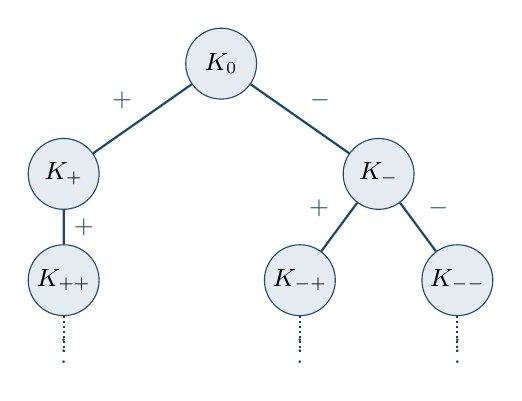
\begin{tikzpicture}[>=Latex,font=\small,
 cnode/.style={circle,draw=manifoldblue!80!black,
 fill=manifoldblue!12,minimum size=9mm,inner sep=1pt}]
 \node[cnode] (r) at (0,2.75) {$K_0$};
 \node[cnode] (a) at (-2,1.35) {$K_+$};
 \node[cnode] (b) at (2,1.35) {$K_-$};
 \node[cnode] (c) at (-2,0) {$K_{++}$};
 \node[cnode] (d) at (1,0) {$K_{-+}$};
 \node[cnode] (e) at (3,0) {$K_{--}$};
 \draw[manifoldblue!80!black,thick]
   (r)--node[above left] {$+$} (a)
   (r)--node[above right] {$-$} (b)
   (a)--node[right] {$+$} (c)
   (b)--node[above left] {$+$} (d)
   (b)--node[above right] {$-$} (e);
 \foreach \x in {c,d,e}{
   \draw[manifoldblue!65!black,densely dotted,thick]
      (\x.south)--++(0,-.45);
 }
 \node[manifoldblue!75!black] at (-2,-.8) {$\vdots$};
 \node[manifoldblue!75!black] at (1,-.8) {$\vdots$};
 \node[manifoldblue!75!black] at (3,-.8) {$\vdots$};
\end{tikzpicture}
\caption{Pierwsze trzy poziomy drzewa. $K_0$ ma
dwa załamania o znakach $+$ i $-$; dlatego w drugim
piętrze są dwa uchwyty. Ich załamania wyznaczają
trzecie piętro. Kropki oznaczają dalsze poziomy,
a nie końcowe wierzchołki.}
\label{fig:casson-signed-tree}
\end{figure}

\begin{przyklad}[Jedna gałąź]
\label{prz:casson-ray}
Jeśli każdy uchwyt ma dokładnie jedno dodatnie
załamanie, drzewo jest nieskończonym promieniem
ze wszystkimi znakami $+$. Każde piętro $T_n$
ma na szczycie jedną pętlę. Zmiana jednego znaku
nie zmienia tego prostego rachunku grupy podstawowej,
choć zmienia dane gładkich plumbowań.
\end{przyklad}

\begin{stwierdzenie}[Co dają skończone piętra]
\label{prop:casson-tower-pi1}
Niech $r_n$ oznacza liczbę punktów podwójnych
na $n$-tym piętrze. Wtedy
$\pi_1(T_n)$ jest grupą wolną na $r_n$ generatorach,
a homomorfizm
$\pi_1(T_n)\to\pi_1(T_{n+1})$ jest zerowy.
W szczególności $\pi_1(CH)=0$.
\end{stwierdzenie}
\begin{proof}
Dla $T_1$ jest to
Stwierdzenie~\ref{prop:casson-first-pi1}.
Załóżmy, że generatory $\pi_1(T_n)$ są pętlami
odpowiadającymi załamaniom najwyższego piętra.
Okrąg przyczepienia każdego nowego uchwytu
reprezentuje dokładnie jeden z tych generatorów.
W nowym uchwycie ten okrąg jest brzegiem jego
immersyjnego rdzenia, a więc staje się
nullhomotopijny. Twierdzenie van Kampena usuwa
wszystkie stare generatory. Pozostają wolne
generatory utworzone przez załamania nowych
uchwytów; ich liczba wynosi $r_{n+1}$.
To kończy indukcję. Każda pętla w $CH$ ma zwarty
obraz, mieści się więc w pewnym $T_n$ i staje się
nullhomotopijna w $T_{n+1}$.
\end{proof}

Ten rachunek nie stwierdza, że $CH$ jest standardowym
otwartym uchwytem $2$. Sama grupa podstawowa nie
rozpoznaje zachowania przy końcu niezwartym ani
lokalnej płaskości ewentualnego dysku granicznego.

\section{Dyski Whitneya i dane w pierścieniu grupowym}
\label{sec:casson-whitney}

Na Rysunku~\ref{fig:freedman-whitney} widzieliśmy
parę punktów przecięcia o znakach $+$ i $-$.
Jeśli odpowiedni okrąg Whitneya jest
nullhomotopijny, można go wypełnić immersyjnym
dyskiem. Ruch Whitneya usuwa wyjściową parę,
gdy wnętrze tego dysku jest czyste i obramowanie
jest właściwe. W wymiarze cztery wnętrze może
przeciąć powierzchnie, a sam dysk może przeciąć
siebie. Przeniesienie problemu na następny dysk
jest ideą wspólną wieżom Cassona i konstrukcjom
z dyskami Whitneya. Są to różne modele geometryczne:
w klasycznej wieży Cassona następne rdzenie
dołącza się do pętli pojedynczych załamań, nie
po prostu do każdej pary punktów Whitneya.

Przy nietrywialnej $\pi_1(M)$ same znaki przecięć
nie wystarczają nawet do znalezienia okręgu
Whitneya, który można wypełnić. Dla dwóch
zorientowanych, obramowanych immersyjnych dysków
lub sfer $A,B$ wybieramy ścieżki od ustalonego
punktu bazowego do ich obrazów. Punkt
$p\in A\cap B$ daje znak $\varepsilon_p\in\{+1,-1\}$
i element $g_p\in\pi_1(M)$: idziemy do $A$,
po $A$ do $p$, a następnie wracamy po $B$.
Otrzymujemy liczbę przecięcia z wartościami w
pierścieniu grupowym
\begin{equation}\label{eq:casson-lambda}
 \lambda(A,B)=\sum_{p\in A\cap B}
             \varepsilon_p g_p\in\Z[\pi_1(M)].
\end{equation}
Przy samoprzecięciu wybór kolejności dwóch płatów
zmienia $g$ na $g^{-1}$. Dlatego obramowana
liczba samoprzecięcia $\mu(B)$ należy do
addytywnego ilorazu
$\Z[\pi_1(M)]/\langle g-g^{-1}:g\in\pi_1(M)\rangle$.
Jest to \emph{niezredukowana} liczba samoprzecięcia:
zachowuje ją homotopia regularna. Dalsze podzielenie
przez podgrupę $\Z\cdot 1$ daje zredukowaną liczbę
\[
 \widetilde\mu(B)\in
 \Z[\pi_1(M)]/
 \bigl(\langle g-g^{-1}:g\in\pi_1(M)\rangle
       +\Z\cdot1\bigr),
\]
która zależy tylko od klasy homotopii. Lokalna
homotopia tworząca lub usuwająca pojedynczy punkt
podwójny z etykietą $1$ zmienia $\mu$, lecz nie
$\widetilde\mu$. Rozróżnienie to będzie istotne przy
porównaniu dwóch wersji twierdzenia o zanurzaniu.
Zależność od orientacji i obramowania oraz definicję
ogólną podają
\href{https://archive.mpim-bonn.mpg.de/4789/2/FreedmanQuinn-TopologyOf4Manifolds-Reformatted2013.pdf}
{Freedman--Quinn, \emph{Topology of 4-Manifolds},
\S\,1.7--1.8}. W przypadku $\pi_1(M)=0$
wartości~\eqref{eq:casson-lambda} są po prostu
całkowitymi liczbami przecięcia.

\begin{stwierdzenie}[Algebraiczne pary punktów]
\label{prop:casson-pairing}
Jeżeli $\lambda(A,B)=0$, punkty $A\cap B$ można
sparować tak, aby w każdej parze znaki były
przeciwne, elementy $g_p$ jednakowe, a okrąg
Whitneya był nullhomotopijny w $M$. Jeżeli
$\lambda(A,B)=1$, po takim parowaniu pozostaje
jeden dodatni punkt o etykiecie $1\in\pi_1(M)$.
\end{stwierdzenie}
\begin{proof}
Pierścień grupowy jest wolną grupą abelową z bazą
$\pi_1(M)$. Zatem współczynnik każdego $g$
w sumie~\eqref{eq:casson-lambda} znika osobno,
z wyjątkiem współczynnika $1$ w drugim przypadku.
Kojarzymy dodatnie i ujemne punkty o tej samej
etykiecie. Dla takiej pary wybieramy łuk od
pierwszego punktu do drugiego na $A$ i łuk
powrotny na $B$. Definicja $g_p$ pokazuje,
że klasa otrzymanej pętli jest iloczynem
$g_p g_q^{-1}=1$. Pętla jest więc nullhomotopijna.
Jej wypełnienie można doprowadzić do położenia
ogólnego jako \emph{immersyjny} dysk Whitneya;
ten ostatni krok nie usuwa jego przecięć wewnętrznych.
\end{proof}

Analogiczna implikacja dla $\mu(B)=0$ wymaga
uwzględnienia zamiany płatów i opisanej relacji
$g\sim g^{-1}$; zob.
Freedman--Quinn, \S\,1.7. Obramowania też
nie można pominąć: skręcenie brzegu dysku
Whitneya może poprawić jego obramowanie,
ale zwykle wytwarza nowe przecięcie z jedną
z powierzchni. Ta algebraiczna redukcja daje
więc \emph{immersyjne} dyski; ich topologiczne
zanurzenie jest następnym, odrębnym krokiem.

\section{Twierdzenie o zanurzaniu dysku}
\label{sec:casson-disk-theorem}

Klasyczny uchwyt Cassona wystarcza w konstrukcji
jednospójnej. Dla nietrywialnej grupy podstawowej
Freedman--Quinn używają dodatkowo powierzchni z
dyskami zamykającymi i uogólnionych wież; warunek
grupowy służy do kontroli pętli punktów podwójnych.
Poniższe twierdzenie nie jest więc formalnym skutkiem
samego rachunku $\pi_1(CH)=0$ ani standardowości
pojedynczego klasycznego uchwytu Cassona.

Grupę $G$ nazywamy \emph{wielostopniowo skończoną
lub cykliczną} (ang. \emph{poly-(finite or cyclic)}),
jeśli ma skończony ciąg
$1=G_0\triangleleft G_1\triangleleft\cdots
\triangleleft G_m=G$, w którym każdy iloraz
$G_{i+1}/G_i$ jest skończony albo nieskończenie
cykliczny.
W szczególności należą tu grupa trywialna,
grupy skończone i $\Z^k$. Jest to konkretna
klasa grup użyta w poniższej wersji twierdzenia.

\begin{twierdzenie}[Freedman--Quinn: zanurzanie dysków;
wynik zewnętrzny]
\label{thm:casson-disk-embedding}
Niech $M^4$ będzie zwartą, spójną, zorientowaną gładką
rozmaitością z brzegiem, a
$A_i:(D^2,S^1)\to(M,\partial M)$,
$1\leq i\leq r$, skończoną rodziną właściwych
immersji obramowanych dysków. Ich brzegi
są parami rozłącznie zanurzone wraz z kołnierzami.
Załóżmy, że istnieją obramowane immersyjne sfery
$B_j:S^2\to\operatorname{int}M$ takie, że w
$\Z[\pi_1(M)]$ zachodzą
\begin{equation}\label{eq:casson-duals}
 \lambda(A_i,B_j)=\delta_{ij},\qquad
 \lambda(B_i,B_j)=0,
\end{equation}
a w grupie samoprzecięć zachodzi $\mu(B_j)=0$
dla każdego $j$. Jeśli $\pi_1(M)$ jest
wielostopniowo skończona lub cykliczna, to w $M$
istnieją parami rozłączne, lokalnie płasko
\emph{topologicznie zanurzone} dyski o tych samych
obramowanych brzegach. Mają one obramowane immersyjne
sfery $B'_j$, homotopijne odpowiednio do $B_j$,
które są geometrycznie dualne: każda $B'_j$ przecina
odpowiedni dysk w jednym punkcie i jest rozłączna
z pozostałymi dyskami.
\end{twierdzenie}

Sfery $B_j$ są \emph{algebraicznie dualne} do
dysków: pierwsza równość w~\eqref{eq:casson-duals}
oznacza jeden punkt przecięcia po skasowaniu
algebraicznych par. Pozostałe warunki kontrolują
przecięcia samych sfer. Obramowanie oznacza tu
trywializację dwuwymiarowej wiązki normalnej,
zgodną z zadanym obramowaniem brzegów dysków.
Twierdzenie podajemy za
\href{https://archive.mpim-bonn.mpg.de/4789/2/FreedmanQuinn-TopologyOf4Manifolds-Reformatted2013.pdf}
{Freedman--Quinn, \emph{Topology of 4-Manifolds},
Twierdzenie 5.2, s.\ 85--87}; w wydaniu książkowym
z 1990 roku jest to Twierdzenie 5.1A. Wersja dla gładkiego
$M$ unika dodatkowego przejścia od rozmaitości
topologicznej do gładkich lokalnych modeli
immersji; to przejście autorzy omawiają
w rozdziale 9. Konkluzja pozostaje topologiczna.
Twierdzenie samo nie mówi, że wyjściowe immersje $A_i$
są homotopijne regularnie do uzyskanych zanurzeń.

W konkluzji słowo \emph{poprzeczne} ma znaczenie
geometryczne: każda uzyskana sfera przecina swój
dysk w dokładnie jednym punkcie, a pozostałe dyski
omija. Samo równanie
$\lambda(A_i,B_j)=\delta_{ij}$ jest słabsze, bo
dopuszcza dodatkowe pary przecięć. W oryginalnym
dowodzie Freedmana--Quinna przejście od dualności
algebraicznej do takich sfer zawierało lukę. Domyka
ją \href{https://arxiv.org/pdf/2006.05209}
{Powell--Ray--Teichner, \emph{The 4-dimensional disc
embedding theorem and dual spheres} (2025),
Twierdzenie A i \S\,5}. Twierdzenie A obejmuje
przytoczoną wyżej wersję dla gładkiego $M$ i grup
wielostopniowo skończonych lub cyklicznych. Jest
sformułowane za pomocą $\widetilde\mu$ i dowolnych
grup dobrych; nasze założenie obramowania oraz
$\mu(B_j)=0$ jest mocniejszym przypadkiem. Nowe
źródło daje sfery $B'_j$ w klasach homotopii $B_j$.
Samo istnienie
zanurzonych dysków wynikało już z wcześniejszej
części argumentu Freedmana--Quinna. Nowe źródło
uzasadnia dodatkową, używaną dalej konkluzję
o \emph{geometrycznie} dualnych sferach.

\begin{stwierdzenie}[Co zapewnia geometryczna dualność]
\label{prop:casson-complement-pi1}
Niech $D_1,\ldots,D_r$ będą parami rozłącznymi,
lokalnie płasko zanurzonymi właściwymi dyskami w
zwartej spójnej rozmaitości $M^4$ z brzegiem.
Jeżeli mają geometrycznie
dualne immersyjne sfery, to inkluzja dopełnienia
indukuje izomorfizm
\[
 \pi_1\bigl(M\setminus\textstyle\bigcup_i D_i\bigr)
       \xrightarrow{\ \cong\ }\pi_1(M).
\]
\end{stwierdzenie}

Jest to własność $\pi_1$-pomijalności wyróżniona w
\href{https://arxiv.org/pdf/2006.05209}
{Powell--Ray--Teichner, Uwaga 1.2}.
\begin{proof}
Przez położenie ogólne każdą pętlę w $M$ można
odsunąć od dysków, więc homomorfizm jest
surjektywny. Niech pętla w dopełnieniu ogranicza
dysk odwzorowany w $M$. Korzystamy tu z
topologicznej transwersalności dla lokalnie
płaskich podrozmaitości oraz z reprezentowania
klas map przez generyczne immersje,
\href{https://arxiv.org/pdf/2006.05209}
{Powell--Ray--Teichner, Twierdzenia 6.4 i 1.5}.
Po uczynieniu odwzorowania poprzecznym do $D_i$
przeciwobrazy
dysków są skończonym zbiorem punktów. Usuwamy
małe kółka wokół tych punktów. Pozostała część
dysku leży w dopełnieniu, a każdy nowy okrąg
brzegowy jest meridianem jednego z $D_i$.
Sfera dualna do $D_i$, po usunięciu małego krążka
otaczającego jej jedyny punkt przecięcia z $D_i$,
daje immersyjny dysk w dopełnieniu, którego brzeg
jest takim meridianem. Wszystkie meridiany są
zatem nullhomotopijne w dopełnieniu, także po
sprzężeniu ścieżkami potrzebnymi do zmiany punktu
bazowego. Doklejenie tych immersyjnych dysków
wypełnia wyjściową pętlę w dopełnieniu. Homomorfizm
jest więc także injektywny.
\end{proof}

Ten prosty skutek wyjaśnia, dlaczego nie wystarcza
zastąpić w konkluzji twierdzenia dualności
geometrycznej dualnością algebraiczną: w drugim
przypadku sfera może mieć kilka punktów przecięcia
z dyskiem, a powyższe wypełnienie meridianu nie
powstaje. Jest to również powód, dla którego
\href{https://arxiv.org/pdf/2006.05209}
{Powell--Ray--Teichner, Uwaga 1.2} podkreślają
kontrolę grupy podstawowej dopełnienia.

\begin{przyklad}[Standardowa para dualna]
\label{prz:casson-dual-product}
Weźmy $M=S^2\times D^2$,
$A=\{p\}\times D^2$ i $B=S^2\times\{0\}$.
Wtedy $\pi_1(M)=0$, dysk i sfera przecinają się
w jednym dodatnim punkcie, $\lambda(A,B)=1$,
a $\mu(B)=0$. Normalne kierunki do obu czynników
dają wymagane obramowania. Twierdzenie obejmuje
tę parę, chociaż tutaj $A$ jest już zanurzony.
Jeżeli $A$ zmienimy we wnętrzu lokalnym ruchem
palcowym, jego brzeg i dualność
algebraiczna nadal pozostają takie same;
nowe punkty podwójne pokazują, jak wyglądają
dane przed zastosowaniem twierdzenia.
\end{przyklad}

\begin{wniosek}[Wersja z homotopią regularną;
wynik zewnętrzny]
\label{cor:casson-regular-homotopy}
Przy założeniach Twierdzenia~\ref{thm:casson-disk-embedding}
załóżmy dodatkowo, że wszystkie algebraiczne
przecięcia wzajemne $A_i$ oraz ich liczby
samoprzecięcia $\mu(A_i)$ są zerowe.
Wtedy rodzinę $A_i$ można przez homotopię
regularną względnie brzegów doprowadzić do
parami rozłącznych topologicznie zanurzonych
dysków z dualnymi sferami.
\end{wniosek}

To jest \href{https://archive.mpim-bonn.mpg.de/4789/2/FreedmanQuinn-TopologyOf4Manifolds-Reformatted2013.pdf}
{Freedman--Quinn, Wniosek 5.2.1, s.\ 87--88};
w wydaniu książkowym jest to Wniosek 5.1B.
Dodatkowych równości dotyczących $A_i$ nie
ukrywamy w Twierdzeniu~\ref{thm:casson-disk-embedding}:
tam potrzebne jest jedynie zachowanie
obramowanych brzegów.

Warto rozdzielić pośrednie kroki tego wniosku.
Równości $\lambda(A_i,A_j)=0$ i $\mu(A_i)=0$
parują algebraicznie przecięcia dysków i pozwalają
wybrać \emph{immersyjne}, odpowiednio obramowane
dyski Whitneya. Najpierw ruchy Whitneya
z użyciem tych dysków
redukują dodatkowe przecięcia $A_i$ ze sferami
algebraicznie dualnymi. Następnie z torusów
opasujących punkty podwójne oraz sfer dualnych
buduje się sfery algebraicznie dualne do samych
dysków Whitneya. Do \emph{nich} stosuje się
Twierdzenie~\ref{thm:casson-disk-embedding},
otrzymując rozłączne zanurzone dyski Whitneya.
Prowadzone po nich ruchy Whitneya usuwają
przecięcia $A_i$; ponieważ są to ruchy wewnątrz,
zachowują obramowane brzegi i dają wskazaną
homotopię regularną. Konstrukcja sfer dualnych
do dysków Whitneya jest częścią zewnętrznego
dowodu Freedmana--Quinna, s.\ 87--88; nie wynika
z samego parowania w pierścieniu grupowym.
Warunek $\mu(A_i)=0$ dotyczy tu niezredukowanej
liczby: właśnie on wyklucza konieczność homotopii
tworzących pojedyncze punkty z etykietą $1$ i pozwala
otrzymać homotopię regularną, a nie tylko dowolną.

Inny ważny znany zakres wyniku stanowią grupy o
wzroście podwykładniczym. Grupa skończenie generowana
ma \emph{wzrost podwykładniczy}, jeśli dla pewnego ---
a równoważnie dla każdego --- skończonego symetrycznego
zbioru generatorów $S$
liczba elementów o długości co najwyżej $n$
spełnia $\lim_{n\to\infty}|B_S(n)|^{1/n}=1$.
Ta własność obejmuje w szczególności grupy
o wzroście wielomianowym. Dla grup podstawowych
o wzroście podwykładniczym tę samą konkluzję
zanurzania otrzymuje się dzięki ulepszeniu
kontroli pętli punktów podwójnych; zob.
\href{https://math.berkeley.edu/~teichner/Papers/Freedman1.pdf}
{Freedman--Teichner, \emph{4-Manifold topology I:
Subexponential groups} (1995)} oraz
\href{https://uva.theopenscholar.com/files/slava-krushkal/files/subexponential_groups.pdf}
{Krushkal--Quinn, \emph{Subexponential groups in
4-manifold topology} (2000)}. Ostatnia praca
podaje poprawiony argument i wskazuje błąd
w pierwotnym dowodzie z 1995 roku. Nie
rozszerzamy stąd twierdzenia na dowolną grupę
podstawową. Jest również wersja z dowolną
$\pi_1(M)$ przy silnym \emph{geometrycznym}
założeniu $\pi_1$-zerowości poprzecznych
powierzchni z dyskami zamykającymi
(Freedman--Quinn, Twierdzenie 5.4).

\section{Gdzie kończy się redukcja geometryczna}
\label{sec:casson-boundary}

Możemy teraz uporządkować rzeczywiście wykonane
kroki. Zerowanie współczynników pierścienia
grupowego pozwala sparować punkty przecięcia
i znaleźć immersyjne dyski Whitneya
(Stwierdzenie~\ref{prop:casson-pairing}).
Samoplumbowanie daje uchwyt pierwszego
piętra z podpisanym znakiem każdego punktu
podwójnego. Dołączanie kolejnych pięter zabija
generatory grupy podstawowej powstałe na
poprzednim piętrze
(Stwierdzenie~\ref{prop:casson-tower-pi1}).
Żaden z tych skończonych rachunków nie produkuje
jeszcze dysku o czystym wnętrzu.

W dowodzie Twierdzenia~\ref{thm:casson-disk-embedding}
potrzeba ponadto skonstruować powierzchnie z
dyskami zamykającymi i dualne sfery, poprawić
grupę podstawową pętli punktów podwójnych,
otrzymać zbieżną wieżę oraz zanurzyć dysk
lokalnie płasko w jej otoczeniu. Są to zasadnicze
zewnętrzne części teorii Freedmana--Quinna:
\href{https://archive.mpim-bonn.mpg.de/4789/2/FreedmanQuinn-TopologyOf4Manifolds-Reformatted2013.pdf}
{\emph{Topology of 4-Manifolds}, rozdziały 2--5}.
Ostatnie przejście opiera się na kontroli
topologicznej przy nieskończonym końcu wieży;
nie wynika z samego van Kampena ani z formalnej
granicy ciągu ruchów Whitneya.

\begin{twierdzenie}[Freedman: standardowość topologiczna
uchwytu Cassona; wynik zewnętrzny]
\label{thm:casson-homeomorphism}
Każdy uchwyt Cassona wraz ze swym obszarem
przyczepienia jest homeomorficzny jako para ze
standardowym otwartym uchwytem $2$:
\[
 (CH,\partial_-CH)\cong
 (D^2\times\R^2,S^1\times\R^2).
\]
Homeomorfizm można dobrać zgodnie z ustalonym
obramowaniem obszaru przyczepienia.
\end{twierdzenie}

Jest to \href{https://www.maths.gla.ac.uk/~mpowell/1982_The%20topology%20of%20four-dimensional%20manifolds.pdf}
{Freedman, \emph{The topology of four-dimensional
manifolds} (1982), Twierdzenie 1.1}.
Przyjmujemy je tutaj jako wynik zewnętrzny.
Jego dowód wymaga ponownego zanurzania wież,
kontroli zbiorów granicznych i argumentów
zmniejszania rozkładów topologicznych. Dopiero
ten wynik uzasadnia przejście od uchwytu Cassona
do standardowego otwartego uchwytu w kategorii
TOP. Nie daje analogicznego dyfeomorfizmu par
w kategorii gładkiej. W szczególności topologiczny
rdzeń $D^2\times\{0\}$ nie musi być gładkim
zanurzonym dyskiem w pierwotnym gładkim $M$.

Twierdzenie o zanurzaniu dysku jest geometrycznym
narzędziem stojącym za topologicznymi wnioskami
Freedmana przytoczonymi w
rozdziale~\ref{ch:freedman-formy}. Wnioski o
gładkich strukturach wymagają osobnych przeszkód;
same znakowane drzewa, wyzerowanie $\pi_1(CH)$
i lokalna płaskość topologiczna ich nie rozstrzygają.

\par\smallskip
{\footnotesize\noindent\emph{Dalsza lektura:}
\href{https://archive.mpim-bonn.mpg.de/4789/2/FreedmanQuinn-TopologyOf4Manifolds-Reformatted2013.pdf}
{M.\ H.\ Freedman i F.\ Quinn, \emph{Topology of 4-Manifolds}},
rozdziały 2--5: uchwyty Cassona i twierdzenie o zanurzaniu dysku;
\href{https://arxiv.org/pdf/2006.05209}
{M.\ Powell, A.\ Ray i P.\ Teichner, \emph{The 4-dimensional
disc embedding theorem and dual spheres}}, korekta argumentu
o sferach dualnych.\par}

\chapter{Klasyfikacja topologicznych rozmaitości czterowymiarowych}
\label{ch:freedman-klasyfikacja}
\index{Freedman!klasyfikacja wymiaru cztery}

W Rozdziale~\ref{ch:freedman-formy} obliczaliśmy formy
przecięcia i oglądaliśmy przeszkodę dla gładkiego
triku Whitneya. Uchwyty Cassona, opisane w
Rozdziale~\ref{ch:uchwyty-cassona}, stanowią drogę
do topologicznego twierdzenia o zanurzaniu dysku.
Poniżej podamy precyzyjny wynik klasyfikacyjny
Freedmana jako wejście zewnętrzne i wyprowadzimy
z niego wnioski. Każde stwierdzenie o homeomorfizmie
dotyczy kategorii TOP; typy gładkie wymagają
osobnych argumentów.

\section{Niezmiennik Kirby'ego--Siebenmanna}
\label{sec:freedman-ks}
\index{niezmiennik Kirby'ego--Siebenmanna}

Niech $X$ będzie zamkniętą, spójną, topologiczną
rozmaitością $4$-wymiarową. Jej stabilna wiązka
styczna jest w kategorii TOP mikrowiązką. Teoria
Kirby'ego--Siebenmanna przypisuje jej klasę
\begin{equation}\label{eq:freedman-ks}
 \operatorname{ks}(X)\in H^4(X;\Z/2).
\end{equation}
Po ewaluacji na mod $2$ klasie fundamentalnej
otrzymujemy liczbę w $\Z/2$, również oznaczaną
$\operatorname{ks}(X)$. Intuicyjnie mierzy ona
przeszkodę do \emph{stabilnego} wygładzenia: dla
zamkniętej rozmaitości $4$-wymiarowej
$\operatorname{ks}(X)=0$ wtedy i tylko wtedy,
gdy $X\times\R$ dopuszcza strukturę gładką.
Jest to wynik zewnętrzny teorii wygładzania,
\href{https://archive.mpim-bonn.mpg.de/4789/2/FreedmanQuinn-TopologyOf4Manifolds-Reformatted2013.pdf}
{Freedman--Quinn, \S\,8.7--8.8 i \S\,10.2.2},
oparty na
\href{https://www.maths.ed.ac.uk/~v1ranick/papers/ks.pdf}
{Kirby--Siebenmann, \emph{Foundational Essays on
Topological Manifolds, Smoothings, and Triangulations}
(1977)}.

W szczególności struktura gładka lub PL na $X$
wymusza $\operatorname{ks}(X)=0$. W wymiarze cztery
odwrotnej implikacji \emph{nie} wolno wyciągać z
tego twierdzenia: zerowanie przeszkody stabilnej
nie buduje automatycznie wygładzenia samego $X$.
Niezmiennik jest zachowywany przez homeomorfizmy,
a dla sum spójnych zachodzi
\[
 \operatorname{ks}(X\#Y)
   =\operatorname{ks}(X)+\operatorname{ks}(Y)
       \quad\text{w }\Z/2.
\]
Te własności również przyjmujemy z powyższego źródła.

Jeżeli $X$ jest dodatkowo jednospójna i zorientowana,
parzystość $Q_X$ odpowiada warunkowi
$w_2(X)=0$: jest to wzór Wu
$Q_X(x,x)\equiv\langle w_2(X),x\rangle\pmod2$
wraz z brakiem $2$-torsji w $H_1(X)$.
Jest to topologiczna wersja warunku spinowego;
również ją przyjmujemy jako wynik zewnętrzny,
\href{https://archive.mpim-bonn.mpg.de/4789/2/FreedmanQuinn-TopologyOf4Manifolds-Reformatted2013.pdf}
{Freedman--Quinn, \S\,10.2.1--10.2.2}.
Bez hipotezy o $H_1$ sama parzystość formy na
całkowitej homologii nie musi wykrywać całego $w_2$.

\section{Twierdzenie Freedmana jako wynik zewnętrzny}
\label{sec:freedman-classification}

\begin{twierdzenie}[Freedman: klasyfikacja jednospójna;
wynik zewnętrzny]
\label{thm:freedman-classification}
Niech $Q$ będzie symetryczną unimodularną formą
całkowitą na wolnej grupie abelowej skończonej rangi,
a $k\in\Z/2$. Jeśli $Q$ jest parzysta, załóżmy
dodatkowo
\begin{equation}\label{eq:freedman-even-ks}
 k\equiv\frac{\sigma(Q)}8\pmod2.
\end{equation}
Wtedy istnieje zamknięta, spójna, zorientowana,
jednospójna \emph{topologiczna} rozmaitość
$X^4$ z $Q_X\cong Q$ i $\operatorname{ks}(X)=k$.
Jeśli $Q$ jest nieparzysta, obie wartości $k=0,1$
są dopuszczalne.

Ponadto dwie takie rozmaitości są homeomorficzne
z zachowaniem orientacji wtedy i tylko wtedy,
gdy ich formy przecięcia są izometryczne i mają
ten sam niezmiennik Kirby'ego--Siebenmanna.
W wersji z ustaloną izometrią form homeomorfizm
można wybrać tak, by indukował właśnie tę izometrię.
\end{twierdzenie}

Wzór~\eqref{eq:freedman-even-ks} ma sens, ponieważ
sygnatura parzystej formy unimodularnej jest podzielna
przez $8$; jak zaznaczono po
Stwierdzeniu~\ref{prop:freedman-E8-properties},
ogólny fakt algebraiczny przyjmujemy z literatury.
Dla jednospójnej $X$ parzystość $Q_X$ oznacza także
$w_2(X)=0$, więc $X$ jest spinowa. W tym przypadku
zewnętrzna formuła dla zamkniętych topologicznych
rozmaitości spinowych brzmi
$\operatorname{ks}(X)\equiv\sigma(X)/8\pmod2$;
zob. Freedman--Quinn, \S\,10.2.2. Wyjaśnia ona
konieczność warunku~\eqref{eq:freedman-even-ks},
natomiast część istnienia Twierdzenia~\ref{thm:freedman-classification}
zapewnia jego wystarczalność.
Oryginalne Twierdzenie 1.5 w pracy
\href{https://www.maths.gla.ac.uk/~mpowell/1982_The%20topology%20of%20four-dimensional%20manifolds.pdf}
{M.\ H.\ Freedman, \emph{The topology of four-dimensional
manifolds}, J. Differential Geom. 17 (1982), 357--453}
jest sformułowane dla rozmaitości gładkich poza jednym
punktem. Podaną wyżej pełną postać w kategorii TOP,
razem z warunkiem na $\operatorname{ks}$, przyjmujemy z
\href{https://archive.mpim-bonn.mpg.de/4789/2/FreedmanQuinn-TopologyOf4Manifolds-Reformatted2013.pdf}
{M.\ H.\ Freedman i F.\ Quinn, \emph{Topology of
4-Manifolds}, \S\,10.1}.
W źródłach dowód korzysta z topologicznego zanurzania
dysków i uchwytów Cassona. Poprzednie sekcje tego
rozdziału nie dowodzą istnienia ani jednoznaczności
homeomorfizmu z twierdzenia.

\section{Dwie konstrukcje w dowodzie Freedmana}
\label{sec:freedman-constructive-examples}
\index{Freedman!konstrukcja rozmaitości o formie $E_8$}

Twierdzenie~\ref{thm:freedman-classification} jest
wynikiem zewnętrznym, ale jego pierwszą konstrukcję
możemy prześledzić na obliczonym już plumbowaniu.
Oddzielimy rachunki homologii i formy od istnienia
topologicznego wypełnienia brzegu. Drugą konstrukcją
będzie rozmaitość o formie $[1]$, której nie da się
odróżnić od $\C P^2$ samą formą przecięcia.

\begin{przyklad}[Od plumbowania do $X_{E_8}$]
\label{prz:freedman-E8-gluing}
Niech $P$ będzie plumbowaniem ośmiu zorientowanych
wiązek $D^2\to P_i\to S^2$ o liczbie Eulera $+2$.
Ich rdzenie są sferami o samoprzecięciu $+2$;
plumbowania wykonujemy według grafu z
Rysunku~\ref{fig:freedman-E8-graph}, wybierając
znaki przecięć sąsiednich rdzeni równe $-1$.
Równoważnie $P$ otrzymujemy z $D^4$ przez osiem
uchwytów $2$ o macierzy sprzężeń $E_8$.
Nie ma uchwytów $1$, zatem $\pi_1(P)=1$, a
Stwierdzenie~\ref{prop:freedman-link-matrix} daje
\[
 H_2(P;\Z)\cong\Z^8,\qquad Q_P=E_8,
 \qquad H_1(\partial P;\Z)=H_2(\partial P;\Z)=0.
\]
Ostatnia równość korzysta z
$\det E_8=1$ ze Stwierdzenia~\ref{prop:freedman-E8-properties}.
Brzeg $\Sigma=\partial P$ jest więc całkowitą
sferą homologiczną. Według Freedmana--Quinna jest
to sfera homologiczna Poincarégo z odpowiednią
orientacją; sam rachunek homologii nie identyfikuje
jej jako $S^3$.

Głęboki krok pochodzi z twierdzenia Freedmana:
\emph{każda} całkowita sfera homologiczna wymiaru
trzy ogranicza kontraktowalną topologiczną
rozmaitość $4$-wymiarową. Wybierzmy takie $C$
z $\partial C\cong-\Sigma$ i sklejmy
\[
 X_{E_8}=P\cup_{\Sigma}C.
\]
Istnienie $C$ jest wynikiem zewnętrznym,
\href{https://www.maths.gla.ac.uk/~mpowell/1982_The%20topology%20of%20four-dimensional%20manifolds.pdf}
{Freedman, \emph{The topology of four-dimensional
manifolds}, twierdzenie $1.4'$}; zob. też
\href{https://archive.mpim-bonn.mpg.de/4789/2/FreedmanQuinn-TopologyOf4Manifolds-Reformatted2013.pdf}
{Freedman--Quinn, wniosek 9.7.2 i \S\,10.5.1}.

Pozostałe kroki są już rachunkami. Twierdzenie
van Kampena opisuje $\pi_1(X_{E_8})$ jako iloraz
$\pi_1(P)*\pi_1(C)$ przez relacje pochodzące od
$\pi_1(\Sigma)$. Oba czynniki są trywialne, bo
$P$ jest jednospójne, a $C$ kontraktowalne;
stąd $\pi_1(X_{E_8})=1$.
Fragment ciągu Mayera--Vietorisa ma postać
\[
 0=H_2(\Sigma;\Z)\longrightarrow
 H_2(P;\Z)\oplus H_2(C;\Z)
 \longrightarrow H_2(X_{E_8};\Z)
 \longrightarrow H_1(\Sigma;\Z)=0.
\]
Ponieważ $H_2(C)=0$, inkluzja $P\hookrightarrow X_{E_8}$
indukuje izomorfizm na $H_2$. Sfery zerowe
plumbowanych wiązek reprezentują bazę $H_2(P)$
i przecinają się we wnętrzu $P$, więc po sklejeniu
zachowują macierz $E_8$. Otrzymaliśmy zatem
zamkniętą, jednospójną rozmaitość topologiczną
o $Q_{X_{E_8}}=E_8$ i $\sigma(X_{E_8})=8$.
Forma jest parzysta, więc $X_{E_8}$ jest spinowa;
zewnętrzny wzór z Sekcji~\ref{sec:freedman-ks}
daje $\operatorname{ks}(X_{E_8})=8/8=1\pmod2$.
To obliczenie wyklucza wygładzenie $X_{E_8}$.
Nie dostarcza ono samodzielnej konstrukcji $C$.
\end{przyklad}

\begin{przyklad}[Drugi typ o formie nieparzystej rzędu jeden]
\label{prz:freedman-odd-twin}
\index{Freedman!drugi typ o formie $[1]$}
Rozważmy $Z=X_{E_8}\#\overline{\C P^2}$. Addytywność
formy i niezmiennika Kirby'ego--Siebenmanna daje
\[
 Q_Z=E_8\oplus[-1],\qquad
 \operatorname{ks}(Z)=1.
\]
Forma $Q_Z$ ma rząd $9$, sygnaturę $7$, jest
nieparzysta i nieokreślona. Klasyfikacja całkowitych
nieparzystych form nieokreślonych daje izometrię
\[
 E_8\oplus[-1]\cong8[1]\oplus[-1].
\]
Jest to twierdzenie algebraiczne cytowane przez
Freedmana--Quinna w \S\,10.2.1; jawny rachunek
odpowiedniej bazy, po odwróceniu znaków, znajduje się
również w Rozdziale~\ref{ch:egzotyczne-r4}.

Wybierzmy w tej izometrii podformę
$7[1]\oplus[-1]$, realizowaną przez gładką
rozmaitość $M=7\C P^2\#\overline{\C P^2}$.
Jej dopełnienie ortogonalne ma formę $[1]$,
na której $w_2$ jest niezerowa, bo kwadrat
generatora jest nieparzysty. Freedman--Quinn
sprawdzają w tym jednospójnym przypadku
pozostałe warunki dotyczące przecięć
i samoprzecięć. Ich zewnętrzne
\emph{twierdzenie o rozkładzie sumy spójnej}
pozwala zrealizować tę podformę jako rozkład
\[
 Z\cong M\#N,\qquad Q_N=[1].
\]
Właśnie ten krok, a nie sama izometria kratek,
korzysta z głębokiej geometrii wymiaru cztery;
zob. \href{https://archive.mpim-bonn.mpg.de/4789/2/FreedmanQuinn-TopologyOf4Manifolds-Reformatted2013.pdf}
{Freedman--Quinn, twierdzenie 10.4 i \S\,10.5.1
w numeracji wersji z 2013 r.}; w wydaniu z 1990 r.
są to twierdzenie 10.3 i dowód twierdzenia 10.1
w \S\,10.4.
Z addytywności otrzymujemy
$\operatorname{ks}(N)=\operatorname{ks}(Z)-
\operatorname{ks}(M)=1$, gdyż $M$ jest gładka.
Ponadto $N$ jest jednospójna na mocy twierdzenia
van Kampena dla sumy spójnej. Ma tę samą formę
$[1]$ co $\C P^2$, lecz inne $\operatorname{ks}$;
stąd nie jest z nią homeomorficzna i nie może
być gładka. Istnienie obu typów w nieparzystym
przypadku Twierdzenia~\ref{thm:freedman-classification}
ma więc konkretny punkt wyjścia w $X_{E_8}$.
\end{przyklad}

\section{Jak zanurzanie dysków wchodzi do klasyfikacji}
\label{sec:freedman-route}

W przypadku jednospójnym grupa podstawowa jest
trywialna, więc spełnia warunek
Twierdzenia~\ref{thm:casson-disk-embedding}.
Twierdzenie to zastępuje odpowiednio przygotowane
immersyjne dyski lokalnie płaskimi zanurzeniami, lecz
\emph{nie} klasyfikuje jeszcze rozmaitości: nie
konstruuje samo formy przecięcia, nie wyznacza
niezmiennika Kirby'ego--Siebenmanna i nie daje
homeomorfizmu między dwiema zadanymi rozmaitościami.

Pierwszym dalszym krokiem jest przejście od dysków
do sfer. W używanej tutaj szczególnej postaci
zewnętrzne \emph{twierdzenie o zanurzaniu sfer} mówi:
jeżeli w spójnej, zorientowanej topologicznej
rozmaitości $M^4$ z $\pi_1(M)=1$ mamy rodzinę obramowanych,
immersyjnych sfer $A_i$ z
$\lambda(A_i,A_j)=0$ dla $i\ne j$ i
$\mu(A_i)=0$, a także obramowane immersyjne sfery
algebraicznie dualne do $A_i$, to rodzinę $A_i$ można
przez homotopię regularną doprowadzić do parami
rozłącznych, lokalnie płasko zanurzonych obramowanych
sfer mających geometrycznie dualne immersyjne sfery.
W tej obramowanej postaci normalna liczba Eulera
$e(A_i)$ wynosi zero. Ponieważ $\pi_1(M)=1$,
to $\lambda(A_i,A_i)=2\mu(A_i)+e(A_i)=0$;
spełniony jest zatem warunek homotopii regularnej,
a zanurzone sfery mają trywialne wiązki normalne.
Jest to szczególny
przypadek \href{https://arxiv.org/pdf/2006.05209}
{Powell--Ray--Teichner, \emph{The 4-dimensional disc
embedding theorem and dual spheres} (2025),
Twierdzenie B i Uwaga 2.2}. W ogólnej postaci twierdzenie
rozróżnia zredukowaną liczbę samoprzecięć od
liczby Eulera normalnego i wymaga $w_2=0$ na
klasach sfer dualnych. Podane tutaj obramowanie
spełnia ten ostatni warunek.

Geometryczna dualność pozwala kontrolować
chirurgię na zanurzonych sferach. Dla jednej
obramowanej sfery $S$ usuwamy
$S^2\times\operatorname{int}D^2$ i wklejamy
$D^3\times S^1$ wzdłuż wspólnego
$S^2\times S^1$. Oznaczmy przez $C$ domknięcie
dopełnienia usuniętego otoczenia, a przez $m$
meridian $S$ w $\partial C$. Twierdzenie van
Kampena daje
\[
 \pi_1(M)\cong\pi_1(C)/\langle\!\langle m\rangle\!\rangle,
 \qquad
 \pi_1(M_{\mathrm{chir}})\cong\pi_1(C),
\]
ponieważ inkluzja $S^2\times S^1\hookrightarrow
D^3\times S^1$ indukuje izomorfizm grup
podstawowych. Gdy $S$ ma
geometrycznie dualną sferę, meridian ogranicza
w $C$ immersyjny dysk, dokładnie jak
w dowodzie Stwierdzenia~\ref{prop:casson-complement-pi1}.
Zatem $m=1$ w $\pi_1(C)$ i chirurgia zachowuje
grupę podstawową.
Jest to jeden z konkretnych powodów, dla których
wniosek o sferach dualnych w twierdzeniu o
zanurzaniu nie jest tylko dodatkiem do jego tezy.

Następne kroki są \emph{zewnętrzne}: algebraiczna
teoria chirurgii organizuje jądra przekształceń
normalnych w pary sfer do zanurzenia; topologiczna
chirurgia w wymiarze cztery używa tych zanurzeń
do usunięcia jądra; twierdzenie o $s$-kobordyzmie
w wymiarze pięć dla dobrej grupy podstawowej
(tu trywialnej) identyfikuje odpowiedni topologiczny
$s$-kobordyzm, którego inkluzje końców są prostymi
równoważnościami homotopijnymi, z produktem.
Dodatkowe argumenty istnienia rozmaitości
o zadanej formie oraz rachunek niezmiennika
Kirby'ego--Siebenmanna domykają klasyfikację.
Dokładne twierdzenia i ich hipotezy znajdują się
u \href{https://archive.mpim-bonn.mpg.de/4789/2/FreedmanQuinn-TopologyOf4Manifolds-Reformatted2013.pdf}
{Freedmana--Quinna, rozdziały 7, 10 i 11},
zwłaszcza Twierdzenie 7.2 oraz \S\,10.1 i \S\,11.6.
Powiązanie tych narzędzi wyjaśnia rolę
Twierdzenia~\ref{thm:casson-disk-embedding},
ale nie jest dowodem
Twierdzenia~\ref{thm:freedman-classification}.

Rysunek~\ref{fig:freedman-classification-route} zbiera
kolejność zależności dla przypadku $\pi_1=1$.
Sfery algebraicznie dualne są częścią danych wejściowych
twierdzenia o zanurzaniu; geometrycznie dualne sfery
są jego wnioskiem. Strzałki oznaczają użycie wyników
zewnętrznych z hipotezami podanymi wyżej, a nie
samodzielną konstrukcję klasyfikacji.

\begin{figure}[htbp]
\centering
\begin{tikzpicture}[
  font=\small,>=Latex,
  routebox/.style={draw=manifoldblue!75!black,
    fill=manifoldblue!7,rounded corners=2pt,
    align=center,text width=3.65cm,minimum height=1.25cm,
    inner sep=4pt},
  routearrow/.style={->,thick,manifoldblue!80!black}]
 \node[routebox] (immersed) at (-5.05,0)
   {immersyjne dyski i sfery; dualność algebraiczna};
 \node[routebox] (towers) at (0,0)
   {wieże Cassona i uogólnienia Freedmana--Quinna};
 \node[routebox] (embedded) at (5.05,0)
   {lokalnie płaskie dyski i sfery; dualność geometryczna};
 \node[routebox] (surgery) at (5.05,-2.1)
   {chirurgia TOP i kontrola $\pi_1$};
 \node[routebox] (cobordism) at (0,-2.1)
   {topologiczny $s$-kobordyzm w wymiarze pięć};
 \node[routebox] (classification) at (-5.05,-2.1)
   {klasyfikacja przez $(Q,\operatorname{ks})$};
 \draw[routearrow] (immersed)--(towers);
 \draw[routearrow] (towers)--(embedded);
 \draw[routearrow] (embedded)--(surgery);
 \draw[routearrow] (surgery)--(cobordism);
 \draw[routearrow] (cobordism)--(classification);
\end{tikzpicture}
\caption{Schemat zależności w przypadku jednospójnym.
Strzałki wymagają zaniku przeszkód algebraicznych i pozostałych
hipotez odpowiednich twierdzeń. Twierdzenia o zanurzaniu
dysków i sfer oraz o topologicznej
chirurgii i $s$-kobordyzmie są wynikami zewnętrznymi.
Realizacja form i rachunek $\operatorname{ks}$ są dodatkowymi
wejściami do ostatniego kroku.}
\label{fig:freedman-classification-route}
\end{figure}

\noindent\textbf{Mechanizm jednoznaczności.}
Niech $M$ i $N$ będą zamkniętymi, zorientowanymi,
jednospójnymi rozmaitościami o izometrycznych
formach i równych niezmiennikach $\operatorname{ks}$.
Twierdzenie Hurewicza utożsamia tu $\pi_2(M)$
z $H_2(M)$, a $\pi_2(N)$ z $H_2(N)$.
W dowodzie Freedmana--Quinna zewnętrzne
twierdzenie o rozkładzie sumy spójnej realizuje
te dane geometrycznie: prowadzi do rozkładu
$N\cong M\#P$ albo do analogicznego rozkładu
wariantu $N$ o przeciwnym $\operatorname{ks}$
w przypadku formy nieparzystej. Dopełnienie $P$
jest jednospójne i ma zerowe $H_2$; dualność
Poincarégo czyni je sferą homologiczną wymiaru
cztery. Topologiczna hipoteza Poincarégo,
również wynik zewnętrzny Freedmana, daje
$P\cong S^4$. Równość $\operatorname{ks}(M)
=\operatorname{ks}(N)$ wybiera pierwszą możliwość;
dla formy parzystej wariant z przeciwnym
$\operatorname{ks}$ nie występuje. To wyjaśnia
rolę obu niezmienników, lecz nie zastępuje dowodu
twierdzenia o rozkładzie ani hipotezy Poincarégo;
zob. \href{https://archive.mpim-bonn.mpg.de/4789/2/FreedmanQuinn-TopologyOf4Manifolds-Reformatted2013.pdf}
{Freedman--Quinn, \S\,10.5.1 i wniosek 7.2.1
w numeracji wersji z 2013 r.}.

\begin{wniosek}[Topologiczna hipoteza Poincarégo w wymiarze cztery]
\label{cor:freedman-poincare-4}
Jeżeli zamknięta, spójna, jednospójna topologiczna
rozmaitość $X^4$ ma homologie całkowite sfery $S^4$,
to $X$ jest homeomorficzna z $S^4$.
W szczególności każda topologiczna sfera homotopijna
wymiaru cztery jest homeomorficzna z $S^4$.
\end{wniosek}
\begin{proof}
Ponieważ $H_4(X;\Z)\cong\Z$, wybieramy orientację.
Warunek homologiczny daje $H_2(X;\Z)=0$, więc
$Q_X$ jest formą zerową na grupie rangi zero.
Jest parzysta, unimodularna w sensie pustej macierzy
o wyznaczniku $1$, i ma sygnaturę $0$.
Z~\eqref{eq:freedman-even-ks} wynika
$\operatorname{ks}(X)=0$. Standardowa $S^4$
ma te same dane, więc część jednoznaczności
Twierdzenia~\ref{thm:freedman-classification}
daje homeomorfizm. Wniosek nie stwierdza
istnienia dyfeomorfizmu.
\end{proof}

\begin{przyklad}[Cztery dane topologiczne]
\label{prz:freedman-examples}
Forma $H$ jest parzysta, ma sygnaturę $0$ i
$\operatorname{ks}=0$, więc jej jedynym zorientowanym
typem topologicznym jest $S^2\times S^2$.
Forma $[1]$ jest nieparzysta: istnieją dokładnie
dwa typy. Jeden to $\C P^2$ z
$\operatorname{ks}=0$; drugi, z
Przykładu~\ref{prz:freedman-odd-twin}, ma
$\operatorname{ks}=1$ i nie może mieć struktury
gładkiej ani PL.

Forma $E_8$ jest parzysta i ma sygnaturę $8$.
Konstrukcja z Przykładu~\ref{prz:freedman-E8-gluing}
daje $X_{E_8}$, a Twierdzenie Freedmana jej
jedyny zorientowany typ topologiczny o tej formie;
a~\eqref{eq:freedman-even-ks} daje
$\operatorname{ks}(X_{E_8})=1$.
Wobec własności z Sekcji~\ref{sec:freedman-ks}
$X_{E_8}$ nie ma struktury gładkiej ani PL.
Natomiast forma $E_8\oplus E_8$ ma sygnaturę $16$,
więc odpowiadający jej typ topologiczny ma
$\operatorname{ks}=0$. Tego ostatniego rachunku
nie interpretujemy jako dowodu gładkości:
Wniosek~\ref{cor:donaldson-2e8} wykluczy
wygładzenie tej rozmaitości za pomocą
twierdzenia Donaldsona.
\end{przyklad}

\begin{table}[htbp]
\centering
\renewcommand{\arraystretch}{1.12}
\setlength{\tabcolsep}{9pt}
\begin{tabular}{@{}lccclc@{}}
\hline
Forma & Parzystość & $\sigma$ & $\operatorname{ks}$
      & Typ TOP & DIFF \\
\hline
$H$ & parzysta & $0$ & $0$ & $S^2\times S^2$ & tak \\
$[1]$ & nieparzysta & $1$ & $0$ & $\C P^2$ & tak \\
$[1]$ & nieparzysta & $1$ & $1$ & $X_{[1],1}$ & nie \\
$E_8$ & parzysta & $8$ & $1$ & $X_{E_8}$ & nie \\
$2E_8$ & parzysta & $16$ & $0$ & $X_{2E_8}$ & nie \\
\hline
\end{tabular}
\caption{Przykłady zamkniętych, spójnych, zorientowanych
i jednospójnych rozmaitości. Każdy wiersz wyznacza dokładnie
jeden typ TOP; $X_{[1],1}$ oznacza drugi typ o formie $[1]$.
W kolumnie DIFF „tak” oznacza istnienie co najmniej jednej
struktury gładkiej, nie jej jednoznaczność.
Brak wygładzenia dla $2E_8$ wynika z
Wniosku~\ref{cor:donaldson-2e8}, mimo że
$\operatorname{ks}=0$.}
\label{tab:freedman-examples}
\end{table}

Twierdzenie~\ref{thm:freedman-classification}
dotyczy tylko zamkniętych, zorientowanych,
jednospójnych rozmaitości w kategorii TOP.
Przypadek ogólnej grupy podstawowej wymaga
dodatkowych danych i hipotez. Własności gładkich
struktur na tej samej topologicznej rozmaitości
wymagają dalszych narzędzi, w szczególności
teorii Donaldsona; żaden rachunek samego
wyznacznika, parzystości i sygnatury ich nie rozstrzyga.

\par\smallskip
{\footnotesize\noindent\emph{Dalsza lektura:}
\href{https://www.maths.gla.ac.uk/~mpowell/1982_The%20topology%20of%20four-dimensional%20manifolds.pdf}
{M.\ H.\ Freedman, \emph{The topology of four-dimensional
manifolds}, J. Differential Geom. 17 (1982), 357--453},
oryginalna konstrukcja;
\href{https://archive.mpim-bonn.mpg.de/4789/2/FreedmanQuinn-TopologyOf4Manifolds-Reformatted2013.pdf}
{M.\ H.\ Freedman i F.\ Quinn, \emph{Topology of
4-Manifolds} (1990)}, zwłaszcza \S\,10.1--10.2:
pełna postać klasyfikacji i niezmiennik
Kirby'ego--Siebenmanna.\par}

\chapter{Gładkie przeszkody Donaldsona w wymiarze cztery}
\label{ch:donaldson}
\index{twierdzenie Donaldsona}
\index{równanie antysamodualności}

Klasyfikacja Freedmana z Rozdziału~\ref{ch:freedman-klasyfikacja}
dotyczy kategorii topologicznej. Pytanie, które z jej przykładów
można wygładzić, wymaga innego narzędzia. Donaldson wykorzystał
połączenia na wiązkach nad gładką rozmaitością czterowymiarową
i analizę ich krzywizny. Poniżej wyprowadzamy równanie
antysamodualności oraz jego prosty rachunek energii. Głębokie
twierdzenie o przestrzeni rozwiązań i wynikającą z niego
diagonalizację podajemy jako wynik zewnętrzny.

\section{Krzywizna połączenia i gwiazda Hodge'a}
\label{sec:donaldson-asd}

Niech $X$ będzie zamkniętą, zorientowaną, gładką
rozmaitością Riemanna wymiaru $4$, a $P\to X$ główną
wiązką o grupie $\mathrm{SU}(2)$. Grupę i jej algebrę
opisuje Dodatek~\ref{sec:app-grupa-u}; połączenia
omawialiśmy w Rozdziale~\ref{ch:koneksje}, a gwiazdę Hodge'a
w Sekcji~\ref{sec:hodge-four-manifolds}.
W lokalnej trywializacji połączenie opisuje
$1$-forma macierzowa $A$ o wartościach w
$\mathfrak{su}(2)$, a jego krzywiznę definiuje wzór
\begin{equation}\label{eq:donaldson-curvature}
 F_A=dA+A\wedge A.
\end{equation}
Iloczyn w drugim składniku łączy iloczyn zewnętrzny form
z mnożeniem macierzy. Dla pól stycznych $u,v$ mamy więc
$(A\wedge A)(u,v)=[A(u),A(v)]$.
Zmiana lokalnej trywializacji nad otwartym $U\subset X$
przez $g:U\to\mathrm{SU}(2)$ daje
$A^g=g^{-1}Ag+g^{-1}dg$ oraz
$F_{A^g}=g^{-1}F_Ag$. Ostatnia równość wynika po
rozwinięciu $d(g^{-1})=-g^{-1}(dg)g^{-1}$:
wyrazy z $dg$ znoszą się parami. Dlatego warunek
na krzywiznę nie zależy od wybranej lokalnej
trywializacji także wtedy, gdy $P$ nie jest trywialna.

W wymiarze cztery gwiazda Hodge'a spełnia
$*^2=1$ na $2$-formach. Dzielimy więc krzywiznę na
\[
 F_A^+=\tfrac12(F_A+*F_A),\qquad
 F_A^-=\tfrac12(F_A-*F_A).
\]

\begin{definicja}[Połączenie antysamodualne]
\label{def:donaldson-asd}
Połączenie $A$ na $P$ jest \emph{antysamodualne},
gdy $F_A^+=0$, czyli $*F_A=-F_A$.
Przestrzeń takich połączeń modulo działanie
gładkich przekształceń cechowania nazywamy
\emph{przestrzenią moduli ASD}.
\end{definicja}

Intuicja jest następująca: gwiazda rozdziela
krzywiznę na dwie niezależne połowy, a równanie
zeruje jedną z nich. Na wiązce trywialnej połączenie
$A=0$ jest płaskie, więc stanowi prosty przykład
rozwiązania.
Nie twierdzimy, że na dowolnej wiązce istnieje
rozwiązanie niepłaskie; zależy to od topologii
wiązki i metryki.

\begin{przyklad}[Niepłaskie rozwiązanie ASD na $\R^4$]
\label{prz:donaldson-asd-lokalny}
Na standardowo zorientowanej euklidesowej $\R^4$
weźmy trywialną wiązkę o grupie $\mathrm{SU}(2)$,
$T=\operatorname{diag}(i,-i)\in\mathfrak{su}(2)$
oraz połączenie opisane globalnie przez
\[
 A=T(x^1\dd x^2-x^3\dd x^4).
\]
Ponieważ wszystkie wartości $A$ są wielokrotnościami
tej samej macierzy, $A\wedge A=0$. Zatem
\[
 F_A=\dd A
   =T(\dd x^1\wedge\dd x^2
       -\dd x^3\wedge\dd x^4).
\]
Dla orientacji $\dd x^1\wedge\cdots\wedge\dd x^4$
gwiazda zamienia $\dd x^1\wedge\dd x^2$
z $\dd x^3\wedge\dd x^4$. Stąd $*F_A=-F_A$,
choć $F_A\ne0$: jest to rozwiązanie ASD, które
nie jest płaskie. Ponieważ $|T|^2=2$ i obie
skalarne $2$-formy są ortonormalne, $|F_A|^2=4$
w każdym punkcie. Jego energia na całej $\R^4$
jest więc nieskończona; poniższa tożsamość
całkowa dotyczy zamkniętej rozmaitości $X$.
\end{przyklad}

\section{Energia i liczba Cherna}
\label{sec:donaldson-energia}

Na $\mathfrak{su}(2)$ przyjmujemy dodatni iloczyn
$\langle B,C\rangle=-\operatorname{tr}(BC)$.
Niech $\|F_A\|_{L^2}^2=\int_X|F_A|^2\,d\mathrm{vol}$.
Niech $E=P\times_{\mathrm{SU}(2)}\C^2$ będzie
stowarzyszoną wiązką zespoloną. Przy konwencji,
w której formą reprezentującą łączną klasę Cherna
jest $c_A(E)=\det(I+\frac{i}{2\pi}F_A)$.
Ponieważ $\mathrm{SU}(2)$ działa z wyznacznikiem $1$,
wiązka $\det E$ jest trywialna i $c_1(E)=0$ także
jako klasa całkowita. Równość $\operatorname{tr}F_A=0$
odzwierciedla to na poziomie form Cherna--Weila.
Współczynnik stopnia cztery w rozwinięciu wyznacznika
ma znak dodatni:
\[
 \frac12\left(\frac{i}{2\pi}\right)^2
 \bigl((\operatorname{tr}F_A)^2
       -\operatorname{tr}(F_A\wedge F_A)\bigr)
 =\frac{1}{8\pi^2}\operatorname{tr}(F_A\wedge F_A).
\]
Dlatego druga liczba Cherna wynosi
\begin{equation}\label{eq:donaldson-c2}
 k=c_2(E)[X]
   =\frac{1}{8\pi^2}\int_X\operatorname{tr}(F_A\wedge F_A)
   \in\Z.
\end{equation}
Całkowitość i niezależność od połączenia są tu
zastosowaniem teorii Cherna--Weila z
Rozdziału~\ref{ch:chern-weil} oraz identyfikacji
otrzymanej formy z całkowitą klasą $c_2(E)$.
Tam wzór na pierwszą klasę Pontriagina wiązki
\emph{rzeczywistej} ma przeciwny znak przy śladzie;
tutaj znak wynika z czynnika $i^2=-1$ w wyznaczniku.
Sam rachunek energii możemy przeprowadzić bez
analizy przestrzeni moduli.

\begin{stwierdzenie}[Rachunek energii ASD]
\label{prop:donaldson-energy}
Dla powyższych konwencji
\[
 \|F_A\|_{L^2}^2
 =8\pi^2k+2\|F_A^+\|_{L^2}^2.
\]
W szczególności dla połączenia antysamodualnego
energia wynosi $8\pi^2k$ i $k\geq0$.
\end{stwierdzenie}
\begin{proof}
Ponieważ $F_A^+$ i $F_A^-$ są ortogonalne,
\[
 |F_A|^2=|F_A^+|^2+|F_A^-|^2.
\]
W zorientowanej bazie ortonormalnej dla skalarnej
$2$-formy $\omega$ zachodzi
$\omega\wedge\omega=\langle\omega,*\omega\rangle
\,d\mathrm{vol}$. Stosując tę równość składowo
do macierzy i znak z definicji iloczynu na
$\mathfrak{su}(2)$, otrzymujemy
\[
 \operatorname{tr}(F_A\wedge F_A)
 =\bigl(|F_A^-|^2-|F_A^+|^2\bigr)
   \,d\mathrm{vol}.
\]
Równość~\eqref{eq:donaldson-c2} daje więc
$8\pi^2k=\|F_A^-\|_{L^2}^2-\|F_A^+\|_{L^2}^2$.
Dodanie $2\|F_A^+\|_{L^2}^2$ kończy dowód.
\end{proof}

Jeżeli $k=0$, każde połączenie ASD na zamkniętym
$X$ jest płaskie: jego energia wynosi zero, więc
ciągła krzywizna znika wszędzie. Przy $k<0$
rozwiązanie ASD nie może istnieć. Dlatego
niepłaski model z
Przykładu~\ref{prz:donaldson-asd-lokalny},
którego energia na całej $\R^4$ jest nieskończona,
nie przeczy temu ograniczeniu.

\section{Twierdzenie o diagonalizacji i jego zakres}
\label{sec:donaldson-diagonalizacja}

Przestrzeń moduli ASD nie jest zwykłą rozmaitością
zadaną skończoną liczbą równań. Trzeba wybrać
warunek cechowania, uzyskać lokalny model eliptyczny,
zbadać rozwiązania redukowalne oraz utratę zwartości
przez koncentrację krzywizny. Zwartość Uhlenbeck,
usuwanie osobliwości i analiza końców przestrzeni moduli
są odrębnymi głębokimi wynikami. Rozdział nie zawiera
ich dowodów.

\begin{twierdzenie}[Donaldson: diagonalizacja formy określonej;
wynik zewnętrzny]
\label{thm:donaldson-diagonalizacja}
Niech $X$ będzie zamkniętą, zorientowaną, gładką,
po prostu spójną rozmaitością wymiaru $4$.
Jeśli całkowita forma przecięcia $Q_X$ na
$H_2(X;\Z)/\operatorname{Tors}$ jest dodatnio określona,
to jest całkowicie izometryczna z
$\langle1\rangle^{\oplus b_2(X)}$.
Jeśli jest ujemnie określona, jest izometryczna z
$\langle-1\rangle^{\oplus b_2(X)}$.
\end{twierdzenie}

Pierwszą wersję otrzymuje się z drugiej po zmianie
orientacji. Źródłem jest
\href{https://doi.org/10.4310/jdg/1214437665}
{S.~K.~Donaldson, \emph{An application of gauge theory to
four-dimensional topology}, J.~Differential Geom. 18 (1983),
twierdzenie~A}. W oryginalnej orientacji dowód bada
połączenia \emph{samodualne} na wiązce z liczbą
$c_2(E)[X]=-1$ nad rozmaitością o dodatnio określonej
formie. Po odwróceniu orientacji gwiazda zmienia znak
na $2$-formach, podobnie jak ewaluacja $c_2(E)[X]$.
Otrzymujemy więc opisaną tutaj konwencję ASD z $k=1$
nad rozmaitością o ujemnie określonej formie.

Dla zrozumienia metody załóżmy teraz, że $Q_X$ jest
ujemnie określona. Rozwiązanie redukowalne odpowiada
rozkładowi $E\cong L\oplus L^{-1}$, dla którego
$1=c_2(E)[X]=-c_1(L)^2[X]$. Takie rozwiązania
odpowiadają zatem parom klas $\{a,-a\}$
o $Q_X(a,a)=-1$. Niech $n(Q_X)$ będzie liczbą tych par.
Odwrotnie, harmoniczny reprezentant każdej takiej klasy
jest antysamodualny, ponieważ forma przecięcia jest
ujemnie określona. Daje on połączenie na $L$ o krzywiźnie
ASD, a $H^1(X;\R)=0$ zapewnia jednoznaczność modulo
cechowanie. Zamiana $L$ na $L^{-1}$ nie zmienia punktu
redukowalnego.
Głęboka część dowodu Donaldsona konstruuje
pięciowymiarową przestrzeń moduli z końcem od
koncentracji krzywizny i punktami redukowalnymi;
rachunek sygnatury jej odpowiednio obciętej wersji
daje $n(Q_X)=b_2(X)$. Ten krok, w tym zwartość,
orientowalność i zachowanie przestrzeni moduli przy
punktach redukowalnych, pozostaje wynikiem zewnętrznym;
por. także \href{https://doi.org/10.1090/S0273-0979-1983-15090-5}
{Donaldson, \emph{Self-dual connections and the topology
of smooth 4-manifolds}, \S\,2--4}.

Końcowy krok jest już algebraiczny. Dla różnych par
$\{a,-a\}$ i $\{b,-b\}$ o kwadracie $-1$ nierówność
Cauchy'ego--Schwarza dla $-Q_X$ daje
$|Q_X(a,b)|\leq1$. Równość oznaczałaby $a=\pm b$,
więc całkowitość formy wymusza $Q_X(a,b)=0$.
Przedstawiciele $n(Q_X)=b_2(X)$ par tworzą zatem
ortogonalny układ pełnej rangi o macierzy $-I$.
Wyznacznik ograniczenia $Q_X$ do generowanej przez
nie podgrupy ma wartość bezwzględną $1$, tak jak
wyznacznik formy $Q_X$. Kwadrat indeksu tej podgrupy
wynosi więc $1$, co czyni ten układ bazą całego
$H_2(X;\Z)/\operatorname{Tors}$. Nie zastępuje to
analitycznej części dowodu Donaldsona.

\begin{wniosek}[Forma $E_8$ nie pochodzi od gładkiej
zamkniętej jednospójnej $4$-rozmaitości]
\label{cor:donaldson-e8}
Nie istnieje zamknięta, gładka, po prostu spójna
rozmaitość $4$-wymiarowa o formie przecięcia $E_8$.
Topologiczna rozmaitość Freedmana o tej formie
nie dopuszcza struktury gładkiej.
\end{wniosek}
\begin{proof}
Z obliczenia w
Stwierdzeniu~\ref{prop:freedman-E8-properties} forma
$E_8$ jest dodatnio określona, parzysta i ma rangę $8$.
Twierdzenie~\ref{thm:donaldson-diagonalizacja}
wymuszałoby izometrię z $I_8$. Ta ostatnia forma
jest nieparzysta, bo wektor bazowy ma kwadrat $1$;
parzystość zachowują izometrie całkowite. To sprzeczność.
Istnienie topologicznej rozmaitości o tej formie jest
częścią zewnętrznego twierdzenia Freedmana przyjętego
w Rozdziale~\ref{ch:freedman-klasyfikacja}.
\end{proof}

\begin{wniosek}[Zniknięcie przeszkody stabilnej
nie wystarcza do wygładzenia]
\label{cor:donaldson-2e8}
Topologiczna, zamknięta, zorientowana, jednospójna
rozmaitość Freedmana $X_{2E_8}$ o formie
$E_8\oplus E_8$ spełnia $\operatorname{ks}(X_{2E_8})=0$,
lecz nie dopuszcza struktury gładkiej.
\end{wniosek}
\begin{proof}
Stwierdzenie~\ref{prop:freedman-E8-properties}
pokazuje, że $E_8$ jest parzysta, unimodularna
i dodatnio określona oraz że $\sigma(E_8)=8$.
Suma prosta dwóch kopii jest więc parzystą,
unimodularną formą dodatnio określoną rangi $16$
o sygnaturze $16$. Twierdzenie
\ref{thm:freedman-classification} daje rozmaitość
topologiczną o tej formie, a warunek
\eqref{eq:freedman-even-ks} daje
$\operatorname{ks}(X_{2E_8})\equiv16/8=2\equiv0\pmod2$,
zgodnie z Przykładem~\ref{prz:freedman-examples}.
Gdyby $X_{2E_8}$ była gładka, Twierdzenie
\ref{thm:donaldson-diagonalizacja} wymagałoby
izometrii $E_8\oplus E_8\cong I_{16}$ nad $\Z$.
Lewa forma jest parzysta, natomiast $I_{16}$
jest nieparzysta, bo wektor bazowy ma kwadrat $1$.
Izometria zachowuje parzystość, więc taka
izometria nie istnieje.
\end{proof}

To porównanie wyostrza Wniosek~\ref{cor:donaldson-e8}:
tam $\operatorname{ks}(X_{E_8})=1$ już wyklucza
gładkość, natomiast tutaj przeszkoda stabilna znika.
Inny wynik zewnętrzny, twierdzenie Rokhlina, mówi,
\index{twierdzenie Rokhlina}
że sygnatura każdej zamkniętej, zorientowanej,
gładkiej rozmaitości spinowej wymiaru cztery
jest podzielna przez $16$;
zob. \href{https://arxiv.org/pdf/2011.12418}
{M.~R.~Klug, \emph{A relative version of Rochlin's theorem},
wprowadzenie}. Gdyby $X_{E_8}$ była gładka,
jej parzysta forma i wzór Wu z
Sekcji~\ref{sec:freedman-ks} czyniłyby ją spinową,
ale sygnatura $8$ naruszałaby ten warunek.
Dla $X_{2E_8}$ sygnatura wynosi $16$, więc
twierdzenie Rokhlina nie wyklucza wygładzenia;
rozstrzyga je dopiero diagonalizacja Donaldsona.

Oba wnioski pokazują precyzyjną granicę między
klasyfikacją topologiczną a gładką. Nie wynika z nich
jeszcze istnienie egzotycznej $\R^4$: potrzebna jest
osobna konstrukcja otwartej rozmaitości i zwarta
przeszkoda rozróżniająca struktury. Przeprowadzimy
wynikającą z niej indukcję w następnym rozdziale.

\par\smallskip
{\footnotesize\noindent\emph{Dalsza lektura:}
\href{https://doi.org/10.4310/jdg/1214437665}
{S.~K.~Donaldson, \emph{An application of gauge theory to
four-dimensional topology}, J.~Differential Geom. 18 (1983)},
twierdzenie o diagonalizacji;
\href{https://doi.org/10.1090/S0273-0979-1983-15090-5}
{S.~K.~Donaldson, \emph{Self-dual connections and the topology
of smooth 4-manifolds}, Bull.~Amer.~Math.~Soc. 8 (1983)},
metoda cechowania i kontekst wyniku.\par}

\chapter{Egzotyczne struktury gładkie na \texorpdfstring{$\R^4$}{R4}}
\label{ch:egzotyczne-r4}
\index{struktura gładka!egzotyczna na $\R^4$}
\index{przestrzeń euklidesowa!egzotyczna $\R^4$}

Z poprzednich rozdziałów znamy już różnicę między
rozmaitością topologiczną a gładką. Klasyfikacja
Freedmana z Rozdziału~\ref{ch:freedman-klasyfikacja}
rozstrzyga pewne pytania o homeomorfizmy, lecz nie
wyznacza atlasu gładkiego. W tym rozdziale wykażemy,
że na przestrzeni topologicznej $\R^4$ istnieje
nieskończenie wiele struktur gładkich, które nie są
ze sobą dyfeomorficzne.

Dowód jest konstrukcją indukcyjną Gompfa. Jego
wejściami są wyniki Freedmana o uchwytach Cassona,
omówionych w Rozdziale~\ref{ch:uchwyty-cassona},
przeszkoda gładka Donaldsona oraz dwa głębokie
lematy Gompfa. Sformułujemy te wejścia jawnie.
Następnie samodzielnie przeprowadzimy krok
indukcyjny i sprawdzimy, dlaczego zwarte podzbiory
rozróżniają otrzymane typy gładkie.

\section{Jak rozróżniać struktury gładkie}
\label{sec:egzotyczne-r4-pojecia}

\begin{definicja}[Egzotyczna $\R^4$]
\label{def:egzotyczna-r4}
Gładka, spójna rozmaitość $R$ jest \emph{egzotyczną
$\R^4$}, jeżeli jest homeomorficzna z topologiczną
$\R^4$, ale nie jest dyfeomorficzna ze standardową
gładką $\R^4$. Dwie struktury gładkie na tej samej
topologicznej $\R^4$ uznajemy za równoważne, gdy
istnieje między nimi dyfeomorfizm.
\end{definicja}

Intuicja: homeomorfizm pozwala używać tych samych
ciągłych współrzędnych globalnych, lecz nie musi
przenosić różniczkowalności. Przykładem odniesienia
jest standardowy atlas na $\R^4$; sama zamiana
globalnych współrzędnych przez dyfeomorfizm
nie daje nowego typu gładkiego. Egzotyczny przykład
otrzymamy dopiero po skonstruowaniu niezanurzalnego
zwartego podzbioru.

W całym dowodzie przestrzenie są zorientowane.
Przez \emph{zanurzenie} rozumiemy gładkie zanurzenie
zachowujące orientację, chyba że wyraźnie napiszemy
inaczej. Odwzorowania topologiczne będziemy tak
nazywać. Rozróżnienie to jest istotne: rezultat
Gompfa najpierw odróżnia typy \emph{zorientowane}.

Niech $K$ będzie zwartą gładką podrozmaitością
czterowymiarową z brzegiem, zanurzoną w $R$.
Jeżeli $K$ nie da się zanurzyć gładko w $R'$, to
nie istnieje gładkie zanurzenie $R\hookrightarrow R'$:
jego ograniczenie do $K$ dałoby zabronione
zanurzenie. Tę prostą obserwację zastosujemy do
ciągu starannie dobranych $K$.

\section{Ślady splotów i sumy przy końcu}
\label{sec:egzotyczne-r4-sploty}

Przypomnijmy terminologię uchwytową z
Definicji~\ref{def:freedman-framed-link}.

\begin{definicja}[Topologicznie plastrowalny splot]
\label{def:egzotyczne-r4-slice}
Splot $L=L_1\sqcup\cdots\sqcup L_s\subset S^3=\partial B^4$
nazywamy \emph{topologicznie plastrowalnym}, jeżeli
jego składowe ograniczają parami rozłączne,
poprawnie i lokalnie płasko zanurzone dyski
$D_i\subset B^4$.
Przez $M_L$ oznaczamy zwartą gładką
czterowymiarową rozmaitość otrzymaną z $B^4$
przez dołączenie do $L$ uchwytów $2$ z obramowaniem
zerowym, mierzonym względem obramowania Seiferta.
\end{definicja}

Lokalna płaskość oznacza, że para $(B^4,D_i)$
w otoczeniu punktu dysku wygląda topologicznie
jak $(\R^4,\R^2)$ lub odpowiedni model przy brzegu.
Istnienie topologicznej wiązki normalnej dla takiego
dysku, również względnie przy brzegu, jest głębokim
\href{https://archive.mpim-bonn.mpg.de/4789/2/FreedmanQuinn-TopologyOf4Manifolds-Reformatted2013.pdf}
{twierdzeniami Freedmana--Quinna (\S\,9.5, tw.~9.6--9.7)}.
Nad $D^2$ wiązka jest trywialna, zatem dyski mają
parami rozłączne otoczenia $D^2\times D^2$.
Gompf równoważnie ujmuje dyski plastra jako
zanurzenia par $(D^2\times\R^2,
\partial D^2\times\R^2)$ w $(B^4,\partial B^4)$;
w tym ujęciu otoczenia należą już do założeń.
Intuicyjnie, rdzenie dołączonych uchwytów w $M_L$
zastępują dyski plastra; ich obramowania muszą
się zgadzać. Przykład stanowi splot złożony z $s$
niezaczepionych okręgów: ograniczają zwykłe,
rozłączne gładkie dyski w $B^4$, a $M_L$ jest
brzegową sumą $s$ kopii $S^2\times D^2$.
Warunek topologicznej plastrowalności nie orzeka,
czy istnieją odpowiednie \emph{gładkie} dyski.
Obramowanie brzegowe dysku plastra ma liczbę
sprzężeń zero z jego brzegiem: równoległy dysk
jest z nim rozłączny. Zgadza się więc z
obramowaniem zerowym użytym w definicji $M_L$.

\begin{stwierdzenie}[Od dysków plastra do śladu]
\label{prop:egzotyczne-r4-slice-trace}
Jeżeli splot $L$ jest gładko plastrowalny,
to $M_L$ zanurza się gładko w standardowej
$\R^4$. Dla dysków tylko lokalnie płaskich
otrzymujemy analogiczne zanurzenie topologiczne.
\end{stwierdzenie}
\begin{proof}
Rozłóżmy $S^4$ na dwie kule $B^4_-$ i $B^4_+$
o wspólnym brzegu $S^3$. Niech dyski plastra leżą
w $B^4_+$. Ich parami rozłączne otoczenia
$D^2\times D^2$ są uchwytami $2$ dołączonymi do
$B^4_-$ wzdłuż $L$. Obramowanie pochodzi z
normalnych dysków i jest zerowe, jak sprawdzono
powyżej. Suma $B^4_-$ z tymi otoczeniami jest
zatem kopią $M_L$ w $S^4$. Wybierając punkt poza
tą zwartą kopią, otrzymujemy zanurzenie w
$S^4\setminus\{\mathrm{punkt}\}\cong\R^4$.
Jeśli orientacje obu półkul dają orientację
przeciwną, składamy zanurzenie z odbiciem $S^4$.
Ten sam argument działa topologicznie dzięki
lokalnej płaskości i topologicznym otoczeniom
dysków. W tym przypadku nie daje gładkiego
zanurzenia $M_L$ w standardowej $\R^4$.
\end{proof}

\begin{przyklad}[Ślad splotu trywialnego]
\label{prz:egzotyczne-r4-unlink}
Dla jednoskładnikowego niewęzła z obramowaniem
zerowym ślad $M_L$ jest dyfeomorficzny z
$S^2\times D^2$. Rdzeń uchwytu $2$ i dysk
ograniczony przez niewęzeł w $B^4$ sklejają się
w sferę generującą $H_2(M_L;\Z)\cong\Z$.
Jej samoprzecięcie wynosi $0$, zgodnie z
obramowaniem, więc forma przecięcia śladu jest
zerowa. Dla splotu $s$ niezaczepionych okręgów
otrzymujemy brzegową sumę $s$ takich śladów;
jej $H_2$ jest równe $\Z^s$, a wszystkie
przecięcia generatorów są zerowe. Ten rachunek
pokazuje, co zapamiętuje obramowanie w prostym
przypadku, ale sam nie rozstrzyga gładkiej
plastrowalności ogólnego splotu.
\end{przyklad}

\begin{definicja}[Ogolona $\R^4$ i suma przy końcu]
\label{def:egzotyczne-r4-shaved}
Gładką rozmaitość $R$ homeomorficzną z $\R^4$
nazywamy \emph{ogoloną} (ang. \emph{shaved}),
jeżeli istnieje jej
gładkie zanurzenie w pewnej gładkiej rozmaitości
$M$ na wnętrze lokalnie płasko zanurzonej
topologicznej zamkniętej kuli $B\subset M$, przy
czym niepusty otwarty fragment $\partial B$ jest
gładką podrozmaitością $M$.

Jeżeli $R=\operatorname{int}B$ oraz
$R'=\operatorname{int}B'$ są tak przedstawione,
umieszczamy $B$ i $B'$ w jednej rozmaitości,
wykonując sumę spójną rozmaitości otaczających
w kulach rozłącznych z $B$ i $B'$.
Wybieramy łuk łączący gładkie fragmenty ich
brzegów. Po dołączeniu cienkiego otoczenia łuku
otrzymujemy brzegową sumę kul; wnętrze nazywamy
\emph{sumą przy końcu} i zapisujemy
$R\mathbin{\natural_\infty}R'$.
\end{definicja}

Cały brzeg $B$ nie musi być gładki: właśnie jego
brak gładkości może przechowywać egzotyczną
strukturę wnętrza. Gładki fragment wystarcza,
by wykonać brzegową sumę. Przykładem ogolonej
rozmaitości jest standardowe $\R^4$, czyli
wnętrze zwykłej gładkiej kuli $B^4\subset S^4$.
Brzegowa suma dwóch zwykłych kul jest znowu
zwykłą kulą, więc odpowiadająca jej suma przy
końcu jest standardową $\R^4$.

\begin{stwierdzenie}[Własności używanej sumy przy końcu]
\label{prop:egzotyczne-r4-suma}
Niech $R,R'$ będą ogolonymi gładkimi rozmaitościami
homeomorficznymi z $\R^4$. Sumę przy końcu można
wybrać tak, by była ogolona i homeomorficzna z
$\R^4$, a zadane zwarte podzbiory $K\subset R$ oraz
$K'\subset R'$ zanurzały się w niej gładko i
rozłącznie. Ponadto $R$ i $R'$ zanurzają się w
tej sumie z zachowaniem orientacji.
\end{stwierdzenie}
\begin{proof}
Po wspomnianej sumie spójnej rozmaitości otaczających
wybierzmy gładkie fragmenty brzegów kul $B,B'$
oraz łuk pomiędzy nimi, nieprzecinający zadanych
zwartych podzbiorów. Otoczenie łuku jest
jednym brzegowym uchwytem $1$ łączącym dwie
topologiczne kule. Ich brzegowa suma jest ponownie
topologiczną kulą $4$-wymiarową: topologicznie
można wyprostować łuk i oglądać dwie kule
połączone cienką rurą. Brzeg pozostaje lokalnie
płaski, a na fragmentach odległych od końców
łuku pozostaje gładki. Wnętrze tej kuli jest
zatem homeomorficzne z $\R^4$ i spełnia definicję
ogolenia. Wnętrza $B$ i $B'$ wchodzą w nie jako
rozłączne gładkie otwarte podrozmaitości, co daje
żądane zanurzenia wraz z $K$ i $K'$.
\end{proof}

Używamy tu \emph{konkretnej} sumy wybranych
modeli. Dla indukcji wystarczy, że istnieje
jeden model sumy przy końcu, w którym oba
wybrane zwarte podzbiory pozostają rozłączne,
a orientacje są zachowane i nie przecinają łuku
sumującego. Pełna niezależność typu gładkiego
od wyboru promieni i łuku nie jest potrzebna
w poniższej konstrukcji; jej dowód znajduje się
w dodatku do pracy Gompfa podanej niżej.

\section{Gładka przeszkoda i trzy wejścia zewnętrzne}
\label{sec:egzotyczne-r4-wejscia}

Mechanizm niezanurzalności bierze początek z
Twierdzenia~\ref{thm:donaldson-diagonalizacja}.
Jego założenia, źródło i rachunek energii równań ASD
omówiliśmy w Rozdziale~\ref{ch:donaldson}.
Samo twierdzenie o
diagonalizacji nie podaje jeszcze zwartego zbioru,
który będzie potrzebny w indukcji.

\begin{twierdzenie}[Gompf: stała przeszkoda zwarta;
wynik zewnętrzny]
\label{thm:egzotyczne-r4-X}
Istnieje zwarta, spójna, zorientowana gładka
czterowymiarowa rozmaitość $X$ o spójnym brzegu
oraz ogolona rozmaitość $R_1$ homeomorficzna
z $\R^4$ takie, że $X$ zanurza się gładko w $R_1$,
lecz $X$ nie zanurza się gładko z zachowaniem
orientacji w żadnej zamkniętej, gładkiej,
jednospójnej czterowymiarowej rozmaitości
o ujemnie określonej formie przecięcia.
\end{twierdzenie}

Taką parę $(X,R_1)$ wybiera
\href{https://doi.org/10.4310/jdg/1214439566}
{R.~E.~Gompf, \emph{An infinite set of exotic
$\R^4$'s}, J.~Differential Geom. 21 (1985),
\S\,1, s.~285--286}, korzystając ze swojej wcześniejszej
\href{https://doi.org/10.4310/jdg/1214437666}
{pracy \emph{Three exotic $\R^4$'s and other
anomalies} (1983)}. Konstrukcja początkowego
$R_1$ wykorzystuje topologiczne uchwyty Cassona
i przeszkodę Donaldsona. Gompf podaje także
konkretną możliwość wyboru $X$: ślad $M_J$
zerowo obramowanego węzła $J$ otrzymanego przez
cztery podwojenia Whiteheada z ujemnymi klamrami
lewoskrętnego węzła trójlistnego. Uzasadnienie
niezanurzalności tego szczególnego $M_J$ wymaga
dodatkowych wyników o uchwytach Cassona; nie
wyprowadzamy go tu z samego diagramu węzła.

Algebraiczne źródło przeszkody jest bardziej
konkretne. We wcześniejszej
\href{https://doi.org/10.4310/jdg/1214437666}
{pracy Gompfa z 1983 roku, s.~321--322}
pojawia się
$M=\C P^2\#9\overline{\C P^2}$ z bazą
$e_0^2=1$, $e_i^2=-1$ i klasą
$x=3e_0+e_1+\cdots+e_8$. Mamy $x^2=9-8=1$.
W podkracie $\Lambda$ rozpiętej przez
$e_0,\ldots,e_8$ klasa $x$ jest charakterystyczna:
dla
$y=a e_0+\sum_{i=1}^8b_i e_i$ zachodzi
$y^2\equiv a+\sum_i b_i\equiv x\cdot y\pmod2$.
Każdy $y\in\Lambda\cap x^\perp$ ma więc parzysty
kwadrat. Ponieważ $x^2=1$, mamy
$\Lambda=\Z x\oplus(\Lambda\cap x^\perp)$;
dopełnienie $x$ jest ujemnie określone,
unimodularne i rangi osiem. Aby rozpoznać
jego macierz bez klasyfikacji kratek określonych,
weźmy
\[
 f_i=e_i-e_{i+1}\quad(1\leq i\leq7),
 \qquad f_8=e_0+e_6+e_7+e_8.
\]
Wektory te należą do $x^\perp$ i mają kwadraty
$-2$. Ponadto $f_i\cdot f_{i+1}=1$ dla
$1\leq i\leq6$ i $f_8\cdot f_5=1$; pozostałe
iloczyny różnych wektorów są zerowe. Po
odwróceniu kolejności $f_1,\ldots,f_7$ ich
macierzą Grama jest $-E_8$ z
Równania~\eqref{eq:freedman-E8}. Ma ona wyznacznik
$1$ na mocy Stwierdzenia~\ref{prop:freedman-E8-properties}.
Ponieważ całe dopełnienie $x$ w $\Lambda$ jest
unimodularne, podkrata o wyznaczniku $1$ ma
indeks $1$; jest więc całą kratą $-E_8$. W całym
$H_2(M;\Z)$ pozostała klasa $e_9$ daje
$x^\perp\cong-E_8\oplus\langle-1\rangle$.
To rachunek w formie \emph{otaczającego} $M$,
nie forma przecięcia zwartego $X$.
Przejście od tej kraty do zakazu zanurzenia $X$
używa konstrukcji uchwytów Cassona i sklejenia
z Lematu~2.3 tamtej pracy; ten krok pozostaje
zewnętrzny. Gompf wybiera zwarty $X$ dopiero
w pracy z 1985 roku, s.~285--286.

\begin{stwierdzenie}[Proste konsekwencje przeszkody]
\label{prop:egzotyczne-r4-X-konsekwencje}
Rozmaitość $X$ z
Twierdzenia~\ref{thm:egzotyczne-r4-X} nie zanurza
się gładko z zachowaniem orientacji w żadnej
gładkiej homotopijnej $4$-sferze. W szczególności
nie zanurza się w standardowej $\R^4$.
\end{stwierdzenie}
\begin{proof}
Gdyby $X\hookrightarrow\Sigma$, gdzie $\Sigma$
jest gładką homotopijną $4$-sferą, wykonajmy
sumę spójną $\Sigma\#\overline{\C P^2}$
w kuli rozłącznej z obrazem $X$. Rozmaitość
ta jest zamknięta, gładka i jednospójna.
Ponieważ $H_2(\Sigma;\Z)=0$, jej forma przecięcia
jest równa $\langle-1\rangle$. Zanurzenie $X$
pozostałoby w tej rozmaitości, co przeczy
Twierdzeniu~\ref{thm:egzotyczne-r4-X}.
Standardowa $\R^4$ zanurza się gładko w $S^4$,
więc także do niej $X$ nie może się zanurzyć.
\end{proof}

\begin{przyklad}[Węzeł plastrowalny topologicznie,
ale nie gładko]
\label{prz:egzotyczne-r4-J}
Niech $J$ będzie czterokrotnym podwojeniem
Whiteheada opisanym po
Twierdzeniu~\ref{thm:egzotyczne-r4-X}, tak że
$X=M_J$. Węzeł $J$ jest topologicznie
plastrowalny: $M_J$ zanurza się w $R_1$,
a homeomorfizm $R_1\cong\R^4$ daje jego
topologiczne zanurzenie w standardowej $\R^4$.
Równoważność między takim zanurzeniem śladu
zerowo obramowanego węzła a topologicznym
dyskiem plastra podaje
\href{https://doi.org/10.4310/jdg/1214439566}
{Gompf, \S\,1, s.~284--285}.
Gdyby $J$ był gładko plastrowalny, ta sama
konstrukcja z gładkim dyskiem dałaby gładkie
zanurzenie $M_J=X$ w standardowej $\R^4$.
Przeczy to
Stwierdzeniu~\ref{prop:egzotyczne-r4-X-konsekwencje}.
\end{przyklad}

\begin{twierdzenie}[Gompf: realizacja śladu splotu;
wynik zewnętrzny]
\label{thm:egzotyczne-r4-slad}
Dla każdego topologicznie plastrowalnego splotu
$L\subset S^3$ istnieje ogolona gładka
rozmaitość $R_L$ homeomorficzna z $\R^4$,
w której $M_L$ zanurza się gładko z zachowaniem
orientacji.
\end{twierdzenie}

Jest to \href{https://doi.org/10.4310/jdg/1214439566}
{lemat~1.1 Gompfa (1985)}. Warto rozdzielić
jego konstrukcję na etapy. Dyski lokalnie płaskie
wyznaczają topologiczne zanurzenie $M_L$ w
$\R^4$ na mocy
Stwierdzenia~\ref{prop:egzotyczne-r4-slice-trace}.
Na obrazie śladu ustalamy atlas, przenosząc go
z gładkiego $M_L$; samo zanurzenie staje się wtedy
gładkie. Dopełnienie wnętrza tego obrazu jest
spójną, niezwartą rozmaitością topologiczną
wymiaru cztery. Twierdzenie Quinna pozwala ją
wygładzić, a jednoznaczność wygładzenia
trójwymiarowego brzegu pozwala skleić oba atlasy
w kołnierzu. Otrzymana gładka rozmaitość jest
topologicznie $\R^4$ i zawiera gładką kopię $M_L$.
Ostatnie \emph{ogolenie} wybiera wnętrze
dostatecznie dużej lokalnie płaskiej kuli,
której otwarty fragment brzegu jest gładki;
zwarty $M_L$ pozostaje w jej wnętrzu.
Gompf uzyskuje taki fragment przez perturbację
homeomorfizmu przy punkcie brzegu, używając
twierdzenia Quinna o stabilnych homeomorfizmach.
Zarówno wygładzanie dopełnienia, jak i ten
ostatni krok pozostają zewnętrzne; zob.
\href{https://www.maths.gla.ac.uk/~mpowell/1982_Ends%20of%20maps%20III.pdf}
{F.~Quinna, \emph{Ends of maps, III: dimensions
4 and 5}, J.~Differential Geom. 17 (1982)}.

\begin{twierdzenie}[Gompf: nowa przeszkoda dla
każdego etapu; wynik zewnętrzny]
\label{thm:egzotyczne-r4-lemat}
Niech $R$ będzie dowolną ogoloną, zorientowaną
gładką rozmaitością homeomorficzną z $\R^4$.
Istnieje topologicznie plastrowalny splot
$L\subset S^3$ taki, że rozłączna suma
$X\sqcup M_L$ nie ma gładkiego zanurzenia
zachowującego orientację w $R$. Tutaj $X$
jest \emph{tym samym} zwartym blokiem co w
Twierdzeniu~\ref{thm:egzotyczne-r4-X}.
\end{twierdzenie}

To dokładnie \href{https://doi.org/10.4310/jdg/1214439566}
{lemat~1.2 Gompfa (1985)}. Hipoteza ogolenia
jest w nim istotna: daje $R\subset B\subset M$,
gdzie $B$ jest lokalnie płaską topologiczną kulą
we wnętrzu gładkiej rozmaitości $M$. Samo
$R\cong_{\mathrm{TOP}}\R^4$ tego nie zapewnia.

\begin{uwaga}[Geometria lematu~1.2]
\label{rem:egzotyczne-r4-mechanizm}
Warto zobaczyć, co wymusza zakaz zanurzenia.
Najpierw Gompf otacza $B$ topologicznym kołnierzem
$S^3\times\R$. Wybiera w nim gładką
trójwymiarową rozmaitość otaczającą $B$
i obcina rozmaitość otaczającą do zwartego fragmentu
$M'$. Ten fragment leży w większej topologicznej
kuli otrzymanej z $B$ i kawałka kołnierza, więc
jest spinowy. Jego podwojenie jest gładkie,
spinowe i ma sygnaturę zero, ponieważ ogranicza
$M'\times I$. Operacje na pętlach poza $B$,
z obramowaniami zachowującymi strukturę spinową,
zabijają grupę podstawową. Forma przecięcia
pozostaje parzysta, unimodularna i ma sygnaturę
zero. Z klasyfikacji form nieokreślonych przywołanej
w Rozdziale~\ref{ch:freedman-formy} wynika, że jest
sumą płaszczyzn hiperbolicznych. Tak otrzymuje zamkniętą,
jednospójną $M$ o formie
$H^{\oplus k}$, gdzie
$H=\bigl(\begin{smallmatrix}0&1\\1&0\end{smallmatrix}\bigr)$.
Istnienie odpowiednich kołnierza, operacji i
reprezentacji hiperbolicznej bazy poza $B$ przez
uchwyty Cassona jest częścią zewnętrznej
konstrukcji Gompfa. Pięć pierwszych pięter
każdego uchwytu jest zwartą wieżą. Rdzenie
szóstego piętra są jeszcze dyskami immersyjnymi;
Gompf przenosi ich samoprzecięcia ku kuli bazowej,
aż rdzenie staną się rozłącznie zanurzonymi
gładkimi dyskami. Dołączenie ich otoczeń do wież
daje gładkie kule $B_i$.
Przecięcia $\partial B_i$ z topologicznymi
sferami reprezentującymi bazę tworzą sploty $L_i$;
ich rozłączna suma w rozłącznych kulach
trójwymiarowych daje poszukiwany $L$.
Gompf zapewnia zgodność obramowań, dodając
w szóstym piętrze tyle samo dodatnich, co
ujemnych samoprzecięć. Dzięki temu można później
wstawić rdzenie uchwytów z $M_L$.
Splot jest topologicznie plastrowalny, ponieważ
odpowiednie uchwyty Cassona są topologicznie
otwartymi uchwytami $2$; jest to dokładnie
Twierdzenie~\ref{thm:casson-homeomorphism}.

Załóżmy teraz, że $X\sqcup M_L$ zanurza się
w $R\subset B$. Oznaczmy przez $B_0$ uchwyt $0$
śladu $M_L$. Rozłączne łuki łączą $B_i$ z $B_0$
poza $X$ i poza konstruowanymi sferami. Otoczenie
sumy $B_0\cup\bigcup_i B_i$ i tych łuków jest
jedną gładką kulą. Na jej brzegu splot utworzony
przez topologiczne fragmenty sfer jest odbiciem
splotu $L$ na brzegu $B_0$. W definicji $L$
Gompf umieszcza sploty $L_i=S_i\cap\partial B_i$
w rozłącznych kulach z odwróconą orientacją
otaczających sfer $S^3$. Oba końce kołnierza
$S^3\times I$ mają przeciwne orientacje brzegowe;
w jego współrzędnych produktowych odpowiadające
sobie składowe są więc kopiami tego samego splotu
i łączą je rozłączne gładkie pierścienie. Sklejamy je
z gładkimi rdzeniami uchwytów $2$ w $M_L$;
tak powstałe dyski zastępują topologiczne fragmenty
sfer. Powstałyby pary gładkich
sfer $S_i,T_i$, z
$S_i^2=T_i^2=0$ i $S_i\cdot T_i=1$,
rozłączne między różnymi parami, reprezentujące
całe $H_2(M;\Z)$. Każda para jest konfiguracją
$S^2\vee S^2$: sfery przecinają się w jednym
punkcie. Jej regularne otoczenie jest
$(S^2\times S^2)\setminus\operatorname{int}B^4$.
Wycięcie tych otoczeń i wklejenie zwykłych
kul $4$ daje gładką homotopijną $4$-sferę,
w której $X$ nadal się zanurza. Jest to sprzeczne
ze Stwierdzeniem~\ref{prop:egzotyczne-r4-X-konsekwencje}.
Istotnie, otoczenia mają brzeg $S^3$ i
reprezentują całe $H_2(M;\Z)$; po ich wycięciu
oraz zaklejeniu brzegu kulami $B^4$ twierdzenia
van Kampena i Mayera--Vietorisa dają odpowiednio
$\pi_1=0$ i $H_2=0$. Dualność Poincarégo
wyznacza pozostałe grupy homologii zamkniętej
rozmaitości, więc ma ona typ homotopijny $S^4$.

Ten opis wskazuje miejsce każdej przeszkody,
ale nie jest dowodem lematu~1.2: konstrukcja
zanurzonych uchwytów Cassona, kontrola obramowań
i rozłączność dysków zajmują istotną część
oryginalnego argumentu Gompfa. Jego głębokie
wejścia pochodzą z
\href{https://www.maths.gla.ac.uk/~mpowell/1982_The%20topology%20of%20four-dimensional%20manifolds.pdf}
{M.~H.~Freedmana, \emph{The topology of
four-dimensional manifolds} (1982)} oraz
\href{https://www.maths.gla.ac.uk/~mpowell/1982_Ends%20of%20maps%20III.pdf}
{Quinna (1982)}.
\end{uwaga}

\section{Indukcja Gompfa i zwarte świadki}
\label{sec:egzotyczne-r4-indukcja}

\begin{twierdzenie}[Nieskończenie wiele struktur
gładkich na $\R^4$]
\label{thm:egzotyczne-r4-nieskonczenie}
Istnieje nieskończenie wiele parami niedyfeomorficznych
gładkich rozmaitości homeomorficznych z $\R^4$.
Można je wybrać spośród rozmaitości Gompfa
$R_0,R_1,R_2,\ldots$, przy czym $R_0$ jest
standardową $\R^4$, a każda $R_n$ dla $n\geq1$
jest egzotyczna.
\end{twierdzenie}
\begin{proof}[Dowód z twierdzeń zewnętrznych
\ref{thm:egzotyczne-r4-X},
\ref{thm:egzotyczne-r4-slad} i
\ref{thm:egzotyczne-r4-lemat}]
Połóżmy $R_0=\R^4$ ze standardową orientacją.
Rozmaitość $R_1$ i jej zwarty podzbiór $X$
pochodzą z Twierdzenia~\ref{thm:egzotyczne-r4-X}.
Stwierdzenie~\ref{prop:egzotyczne-r4-X-konsekwencje}
pokazuje, że nie ma zanurzenia $R_1\hookrightarrow R_0$.

Załóżmy, że ogolona $R_{n-1}$, zawierająca
gładko $X$, została już zbudowana, gdzie $n\geq2$.
Z Twierdzenia~\ref{thm:egzotyczne-r4-lemat}
wybieramy splot $L_n$ taki, że zwarta
rozłączna suma
\begin{equation}\label{eq:egzotyczne-r4-Kn}
 K_n:=X\sqcup M_{L_n}
 \quad\text{nie zanurza się gładko w }R_{n-1}.
\end{equation}
Twierdzenie~\ref{thm:egzotyczne-r4-slad}
daje ogoloną $R_{L_n}$ z zanurzonym
$M_{L_n}$. Tworzymy
\begin{equation}\label{eq:egzotyczne-r4-Rn}
 R_n:=R_{n-1}\mathbin{\natural_\infty}R_{L_n}.
\end{equation}
Łuk sumowania wybieramy z dala od $X$ i
$M_{L_n}$. Stwierdzenie~\ref{prop:egzotyczne-r4-suma}
zapewnia, że $R_n$ jest ogolona,
homeomorficzna z $\R^4$, zawiera $R_{n-1}$
oraz zawiera rozłącznie zanurzone oba składniki
$K_n$. W szczególności w $R_n$ nadal jest $X$,
więc krok można powtarzać.

Gdyby istniało gładkie zanurzenie zachowujące
orientację $R_n\hookrightarrow R_{n-1}$,
jego ograniczenie do $K_n$ przeczyłoby
\eqref{eq:egzotyczne-r4-Kn}. Zatem
$R_n\not\hookrightarrow R_{n-1}$.
Dla $m<n$ mamy natomiast zanurzenia
$R_m\hookrightarrow R_{m+1}\hookrightarrow
\cdots\hookrightarrow R_{n-1}$. Gdyby
$R_n\hookrightarrow R_m$, ich złożenie
dałoby wykluczone zanurzenie
$R_n\hookrightarrow R_{n-1}$. Otrzymaliśmy
więc nieskończenie wiele parami różnych
\emph{zorientowanych} typów dyfeomorfizmu.
Każda $R_n$ dla $n\geq1$ jest egzotyczna:
gdyby była dyfeomorficzna ze standardową
$R_0$ z zachowaniem orientacji, mielibyśmy
zanurzenie $R_n\hookrightarrow R_0$. Jeśli
dyfeomorfizm odwracałby orientację, można
złożyć go z odbiciem standardowej $\R^4$;
wynik byłby dyfeomorfizmem zachowującym
orientację, co prowadzi do tej samej sprzeczności.

Trzeba jeszcze sprawdzić tezę bez warunku
zachowania orientacji. Jeden niezorientowany
typ dyfeomorfizmu ma najwyżej dwa typy
zorientowane: odpowiadają one dwóm wyborom
orientacji. Gdyby wśród $R_n$ występowało
tylko skończenie wiele typów niezorientowanych,
byłoby także tylko skończenie wiele typów
zorientowanych. Jest ich nieskończenie wiele,
więc istnieje nieskończony podciąg $R_{n_j}$
parami niedyfeomorficzny nawet po dopuszczeniu
odwrócenia orientacji.
Możemy włączyć do tego podciągu $R_0$.

Na koniec wybierzmy dla każdego $j$ homeomorfizm
$h_j:\R^4\to R_{n_j}$ i przenieśmy atlas gładki
$R_{n_j}$ na tę samą topologiczną przestrzeń
$\R^4$. Dyfeomorfizm między dwoma przeniesionymi
atlasami dałby dyfeomorfizm między odpowiednimi
$R_{n_j}$. Takiego dyfeomorfizmu nie ma, więc
otrzymane struktury gładkie są parami nierównoważne.
\end{proof}

\begin{figure}[htbp]
\centering
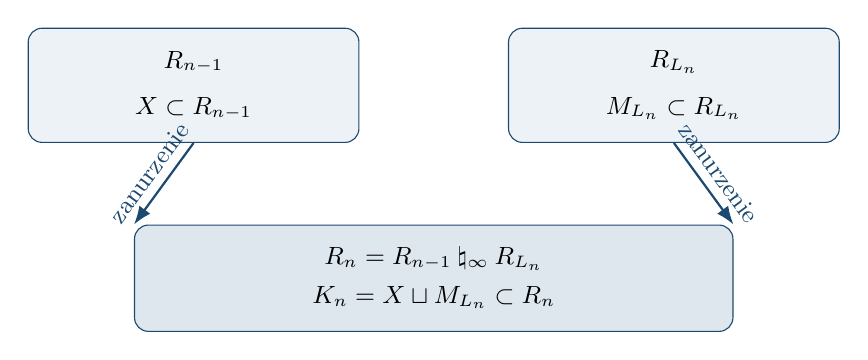
\begin{tikzpicture}[font=\small,>=Latex,
  every node/.style={align=center}]
 \node[draw=manifoldblue!80!black,rounded corners=5pt,
       fill=manifoldblue!8,minimum width=4.2cm,
       minimum height=1.45cm] (old) at (-3.05,1.35)
       {$R_{n-1}$\\[2mm]$X\subset R_{n-1}$};
 \node[draw=manifoldblue!80!black,rounded corners=5pt,
       fill=manifoldblue!8,minimum width=4.2cm,
       minimum height=1.45cm] (new) at (3.05,1.35)
       {$R_{L_n}$\\[2mm]$M_{L_n}\subset R_{L_n}$};
 \node[draw=manifoldblue!80!black,rounded corners=5pt,
       fill=manifoldblue!15,minimum width=7.6cm,
       minimum height=1.35cm] (sum) at (0,-1.1)
       {$R_n=R_{n-1}\mathbin{\natural_\infty}R_{L_n}$\\[1mm]
        $K_n=X\sqcup M_{L_n}\subset R_n$};
 \draw[->,thick,manifoldblue!80!black] (old.south)
       -- node[left,sloped,above] {zanurzenie} (sum.north west);
 \draw[->,thick,manifoldblue!80!black] (new.south)
       -- node[right,sloped,above] {zanurzenie} (sum.north east);
\end{tikzpicture}
\caption{Schemat indukcji Gompfa: oba zanurzenia
umieszczają $K_n=X\sqcup M_{L_n}$ w $R_n$.
Rysunek nie przedstawia egzotycznego końca.}
\label{fig:egzotyczne-r4-indukcja}
\end{figure}

Rysunek~\ref{fig:egzotyczne-r4-indukcja} pokazuje
rolę zwartego świadka: $K_n$ \emph{zanurza się}
w $R_n$, lecz \emph{nie zanurza się} w $R_{n-1}$.
Sama odmienność diagramów splotów $L_n$ nie
rozróżniałaby rozmaitości. Silniejsze
\href{https://doi.org/10.4310/jdg/1214439566}
{twierdzenie~1.3 Gompfa} obejmuje ponadto graniczną
rozmaitość $R_\infty$. Dla skończonych indeksów
$m,n\in\N_0$ powyższy dowód daje porządek
zorientowanych zanurzeń:
$R_m\hookrightarrow R_n$ wtedy i tylko wtedy,
gdy $m\leq n$.

\section{Małe i duże egzotyczne \texorpdfstring{$\R^4$}{R4}}
\label{sec:egzotyczne-r4-male-duze}
\index{przestrzeń euklidesowa!mała egzotyczna $\R^4$}
\index{przestrzeń euklidesowa!duża egzotyczna $\R^4$}

Egzotyczna $\R^4$ jest \emph{mała}, gdy zanurza
się gładko w standardowej $\R^4$, i \emph{duża}
w przeciwnym razie. Przy równości wymiarów
zanurzenie jest dyfeomorfizmem na otwarty
podzbiór celu. Nazwy nie dotyczą rozmiaru
metrycznego.

\begin{twierdzenie}[De Michelis--Freedman:
małe egzotyczne $\R^4$; wynik zewnętrzny]
\label{thm:egzotyczne-r4-male}
Istnieje rodzina mocy kontinuum otwartych
podzbiorów standardowej $\R^4$, z których
każdy jest homeomorficzny z $\R^4$, a każde
dwa są niedyfeomorficzne.
\end{twierdzenie}

Wynik ten pochodzi z
\href{https://doi.org/10.4310/jdg/1214447810}
{S.~De Michelisa i M.~H.~Freedmana,
\emph{Uncountably many exotic $\R^4$'s in
standard 4-space}, J.~Differential Geom. 35
(1992), 219--254}. Dowód jest osobnym głębokim
wejściem. Po usunięciu co najwyżej jednego typu
standardowego pozostaje kontinuum małych
egzotycznych $\R^4$. Każda skonstruowana wyżej
$R_n$ dla $n\geq1$ jest natomiast duża: zawiera
$X$, które nie zanurza się w standardowej $\R^4$.
Zanurzenie odwracające orientację po złożeniu
z odbiciem celu także przeczyłoby tej przeszkodzie.

\par\smallskip
{\footnotesize\noindent\emph{Dalsza lektura:}
\href{https://doi.org/10.4310/jdg/1214439566}
{R.~E.~Gompf, \emph{An infinite set of exotic $\R^4$'s}},
§1: lematy konstrukcyjne i pełne twierdzenie o rodzinie;
\href{https://doi.org/10.4310/jdg/1214447810}
{S.~De Michelis i M.~H.~Freedman,
\emph{Uncountably many exotic $\R^4$'s in standard 4-space}},
małe egzotyczne struktury.\par}


\part{Dodatki}
\appendix
\chapter{Zależności zewnętrzne i poziom samowystarczalności}
\label{app:wyniki-zewnetrzne}

W skrypcie dowód oznacza rzeczywiste
wyprowadzenie ze wskazanych wcześniejszych
faktów. Jeśli korzystamy z długiego
twierdzenia spoza tekstu, podajemy
hipotezy, miejsce użycia i źródło.
Poniższy katalog ułatwia rozpoznanie
tych punktów zależności.

\section{Wyniki wejściowe i głębokie lematy}
\label{sec:katalog-wynikow}

\begin{description}[leftmargin=2.9cm,style=nextline]
\item[Niezmienniczość obszaru.]
  Ciągła injekcja z otwartego
  $U\subset\R^n$ do $\R^n$
  ma otwarty obraz. Użyta w
  Rozdziale~\ref{ch:rozmaitosci}
  do niezależności wymiaru i
  brzegu od map.
  Źródło:
  \href{https://pi.math.cornell.edu/~hatcher/AT/AT.pdf}
  {A.\ Hatcher, \emph{Algebraic Topology},
  twierdzenie 2B.3}.
  Alternatywny dowód samej
  niezmienniczości wymiaru rozmaitości
  przez homologię lokalną jest poniżej.

\item[Twierdzenie o funkcji odwrotnej.]
  Dla $C^1$ odwzorowania między
  otwartymi podzbiorami $\R^n$
  z odwracalną pochodną w punkcie
  istnieje lokalna odwrotność $C^1$;
  dla danych $C^\infty$ jest ona
  $C^\infty$. Użyte przy mapach,
  zanurzeniach i funkcjach Morse'a.
  Źródło z dowodem:
  \href{https://www.ocw.mit.edu/courses/18-101-analysis-ii-fall-2005/d2c8fc5fe57cd59efc99caa048983d4c_lecture6.pdf}
  {V.\ Guillemin, \emph{Analysis II},
  wykład 6}.

\item[Miara Hausdorffa w przestrzeni euklidesowej.]
  Identyfikacja znormalizowanej miary Hausdorffa
  $\mathcal H^k$ na $\R^k$ z miarą Lebesgue'a,
  użyta w Rozdziale~\ref{ch:metryka-riemannowska},
  korzysta z nierówności izodiametrycznej i z twierdzenia
  Vitalego o pokryciu. Sam rachunek normalizacji oraz
  zastosowanie w mapach rozmaitości są w rozdziale,
  natomiast te dwa fakty miarowe pozostają zewnętrzne.
  Źródło:
  \href{https://www.math.cmu.edu/~gautam/sj/teaching/2022-23/720-measure/pdfs/measure.pdf}
  {G.\ Iyer, \emph{Lecture Notes on Measure Theory},
  dodatek A}.

\item[Triangulacja gładka.]
  Każda gładka rozmaitość
  drugoprzeliczalna dopuszcza
  triangulację zgodną ze
  strukturą gładką; w przypadku
  zwartym może być skończona.
  Używamy jej do przejścia od
  geometrii do skończonych
  kompleksów łańcuchowych.
  Źródło:
  \href{https://www.ams.org/bull/1935-41-08/S0002-9904-1935-06140-3/S0002-9904-1935-06140-3.pdf}
  {S.~S.\ Cairns, \emph{Triangulation of the
  Manifold of Class One}, §1--2}, oraz
  \href{https://doi.org/10.2307/1968861}
  {J.~H.~C.\ Whitehead, \emph{On $C^1$-complexes}}.
  Pełny dowód nie jest krótkim
  uzupełnieniem tego skryptu.

\item[Kohomologia Čech i singularna.]
  Każde pokrycie rozmaitości ma
  rozdrobnienie będące dobrym pokryciem.
  Dobre pokrycia tworzą więc rodzinę
  kofinalną w definicji kohomologii
  Čecha. Dla dobrego pokrycia kompleks
  Čecha oblicza kohomologię nerwu,
  a lemat o nerwie utożsamia jego
  typ homotopijny z rozmaitością.
  Dla współczynników w dyskretnej
  grupie abelowej otrzymujemy stąd
  izomorfizm kohomologii Čecha
  i singularnej. Interpretacja
  kocyklu przejść struktury
  spinowej w Rozdziale~\ref{ch:grass-spin}
  używa tego porównania;
  tam, gdzie wystarcza stopień
  pierwszy, podano też argument
  przez monodromię pętli.
  Istnienie dobrych pokryć opisują
  \href{https://doi.org/10.1007/978-1-4757-3951-0}
  {R.\ Bott i L.~W.\ Tu, \emph{Differential Forms in
  Algebraic Topology}, §5}. Wybierając użyte tam dostatecznie
  małe geodezyjnie wypukłe kule podporządkowane zadanemu pokryciu,
  otrzymujemy dobre rozdrobnienie; to daje potrzebną kofinalność.
  Pozostałe składniki porównania:
  \href{https://pi.math.cornell.edu/~hatcher/AT/AT.pdf}
  {A.\ Hatcher, \emph{Algebraic Topology},
  wniosek 4G.3 o nerwie dobrego pokrycia
  oraz §2.1 i §3.1 o kohomologii
  symplicjalnej i singularnej}.

\item[Trik Whitneya i ruchy uchwytów.]
  Niech $P^r,Q^s$ będą domkniętymi, poprzecznie
  przecinającymi się gładkimi podrozmaitościami
  $V^{r+s}$ bez brzegu; orientujemy $P$ i wiązkę
  normalną $Q$. Usunięcie punktów przecięcia $u,v$
  o przeciwnych znakach wymaga $r\geq2$, $s\geq3$
  i $r+s\geq5$. Łuki łączące $u,v$ w $P$ i $Q$
  mają wnętrzami omijać pozostałe przecięcia, a utworzony
  przez nie okrąg ma być ściągalny w $V$. Przy $r=2$
  zakładamy ponadto injektywność
  $\pi_1(V\setminus Q)\to\pi_1(V)$. Konstrukcja daje
  odpowiednio obramowany dysk Whitneya i izotopię
  usuwającą tę parę przecięć.
  Użyte w
  Rozdziałach~\ref{ch:hcobordyzm}--\ref{ch:przeszkoda-chirurgiczna}.
  Źródło warunków i konstrukcji:
  \href{https://www.math.columbia.edu/~jmorgan/Lecture_IIIA_hcobordism_Contd.pdf}
  {J.\ Morgan, \emph{The $h$-Cobordism Theorem},
  wykład IIIA}, oraz
  \href{https://webhomes.maths.ed.ac.uk/~v1ranick/surgery/hcobord.pdf}
  {J.\ Milnor, \emph{Lectures on the $h$-Cobordism Theorem},
  twierdzenie 6.6 i lematy 6.7, 6.13}.

\item[Dwie chirurgii okręgu w $S^4$.]
  Dla standardowego okręgu dwa zorientowane obramowania
  dają produktową i nietrywialną wiązkę $S^2$ nad $S^2$.
  Rozdział~\ref{ch:chirurgia-geometryczna-21} oblicza ich formy
  przecięcia; identyfikacja nietrywialnej wiązki z
  $\mathbb{CP}^2\#\overline{\mathbb{CP}^2}$ pozostaje wejściem z
  \href{https://arxiv.org/abs/1502.06834}
  {K.\ Larsona, \emph{Surgery on tori in the 4-sphere},
  dowód propozycji 4.3} oraz
  \href{https://www.mathematik.hu-berlin.de/~wendl/pub/rationalRuled.pdf}
  {C.\ Wendla, \emph{Holomorphic Curves in Low Dimensions},
  przykład 1.11 i uwaga 1.13}.
  Nie jest to zastosowanie wysokowymiarowego
  twierdzenia Walla.

\item[Torsja Whiteheada i $s$-kobordyzm.]
  Dla równoważności homotopijnej spójnych skończonych
  kompleksów CW zerowanie torsji Whiteheada jest równoważne
  prostocie tej równoważności. Wynik ten stosujemy w
  Rozdziale~\ref{ch:s-kobordyzm}; źródło:
  \href{https://webhomes.maths.ed.ac.uk/~v1ranick/papers/owsem.pdf}
  {M.\ Kreck i W.\ Lück, \emph{The Novikov Conjecture},
  twierdzenie 6.15(1)}. Drugim wejściem jest utożsamienie
  torsji uporządkowanego kompleksu Morse'a z torsją
  komórkową zgodnej gładkiej triangulacji oraz niezależność
  tej klasy od triangulacji; zob.
  \href{https://webhomes.maths.ed.ac.uk/~v1ranick/papers/milnorwh.pdf}
  {J.\ Milnor, \emph{Whitehead Torsion}, lemat 9.1
  i twierdzenie 9.3}. Po tych wejściach rozdział dowodzi,
  że dla spójnego zwartego gładkiego $h$-kobordyzmu
  $(W^m;N_-,N_+)$ o niepustych, spójnych i zamkniętych
  brzegach, $m\geq6$, zachodzi
  $\tau(W,N_-)=0$ wtedy i tylko wtedy, gdy
  $W\cong N_-\times I$ relatywnie do $N_-$;
  orientowalność nie jest założeniem.
  Przykład 6.6 Milnora oblicza osobno
  $\operatorname{Wh}(C_5)\cong\Z$ z generatorem
  $[1-t-t^{-1}]$; używamy go w
  Przykładzie~\ref{prz:Tate-C5-22}.

\item[Twierdzenia Walla.]
  Niech $(f,b):M^n\to X^n$ będzie normalnym
  odwzorowaniem stopnia jeden między spójnymi,
  zamkniętymi, gładkimi rozmaitościami, $n\geq5$,
  z charakterem orientacji $w$ na
  $\pi=\pi_1(X)$. Przeszkoda
  $\theta(f,b)\in L_n^s(\Z[\pi],w)$ znika wtedy
  i tylko wtedy, gdy $(f,b)$ jest normalnie
  kobordantne z prostą równoważnością homotopijną.
  W wersji zwartej z brzegiem odwzorowanie brzegowe
  ma być prostą równoważnością, a kobordyzm i chirurgie
  wykonuje się relatywnie do brzegu. Przypadek parzysty
  $n=2k\geq6$ daje twierdzenie 5.6 Walla, a przypadek
  nieparzysty $n=2k+1\geq5$, obejmujący wymiar pięć,
  daje twierdzenie 6.4; nie należy go mylić z nieparzystym
  twierdzeniem realizacyjnym 6.5, którego zakres zaczyna
  się w wymiarze siedem.

  Rozdział~\ref{ch:przeszkoda-chirurgiczna}
  rozpisuje rachunek przecięć i konstrukcję
  bazy hiperbolicznej nad $\Z[\pi]$,
  chirurgie poniżej środka, ciągi dokładne jąder,
  dualność oraz część ruchów formacji. Osobnymi
  wejściami pozostają przygotowanie kobordyzmu,
  bazowość i prosta dualność jego jąder,
  realizacja względnych immersji, geometryczne lematy
  Walla oraz pełna realizacja ruchów nieparzystych.

  Wersja z jedynie zwykłą równoważnością na brzegu ma
  przeszkodę $\theta^h(f,b)\in L_n^h(\Z[\pi],w)$.
  Homomorfizm zapominający prostotę
  $L_n^s\to L_n^h$ i jego związek z grupą
  Whiteheada opisuje ciąg dokładny Rothenberga z grupami
  Tate'a $\widehat H^*(\Z/2;\operatorname{Wh}(\pi))$.
  Te twierdzenia są zewnętrzne; zob.
  \href{https://www.maths.ed.ac.uk/~v1ranick/surgery/ranicki.pdf}
  {A.\ Ranicki, \emph{An Introduction to Algebraic Surgery},
  wstęp i przykład 2.16},
  \href{https://webhomes.maths.ed.ac.uk/~v1ranick/books/scm.pdf}
  {Walla, §17D}.

  Osobnym wejściem jest rozszczepienie Shanesona--Ranickiego
  $L_n^s(\Z[G\times\Z],w\oplus1)
   \cong L_n^s(\Z[G],w)\oplus L_{n-1}^h(\Z[G],w)$
  dla dodatkowego generatora zachowującego orientację.
  W przypadku $G=1$ prowadzi ono do tabeli
  $L_n^s(\Z[t,t^{-1}],1)$ w
  Sekcji~\ref{sec:L-pi1-Z-22}. Źródła:
  \href{https://webhomes.maths.ed.ac.uk/~v1ranick/papers/shan.pdf}
  {J.\ Shaneson, \emph{Wall's Surgery Obstruction Groups
  for $G\times\Z$}, twierdzenie 5.1, wariant geometryczny
  dla $G=\pi_1(K^{n-2})$, $w=w_1(K)$, $n\geq7$
  i zamkniętej gładkiej lub PL rozmaitości $K$} oraz
  \href{https://webhomes.maths.ed.ac.uk/~v1ranick/papers/splitkl.pdf}
  {A.\ Ranicki, \emph{Algebraic and Geometric Splittings
  of the K- and L-Groups of Polynomial Extensions}, §6,
  wariant algebraiczny dla dowolnej grupy}.

  Dla spójnej zamkniętej gładkiej $X^n$, $n\geq5$,
  identyfikacja $\mathcal N_{\mathrm{DIFF}}(X)\cong[X,G/O]$,
  działanie $L_{n+1}^s$ na prostym zbiorze struktur i ciąg
  chirurgii
  \[
   [\Sigma X_+,G/O]\longrightarrow
   L_{n+1}^s(\Z[\pi],w)
   \longrightarrow\mathcal S^s_{\mathrm{DIFF}}(X)
   \longrightarrow[X,G/O]\longrightarrow
   L_n^s(\Z[\pi],w)
  \]
  są kolejnymi zewnętrznymi wynikami Walla użytymi w
  Rozdziale~\ref{ch:ciag-chirurgii}. Realizacja elementów
  $L_{n+1}^s$ korzysta z twierdzenia 5.8 dla parzystego
  $n+1\geq6$ oraz z twierdzenia 6.5 dla nieparzystego
  $n+1\geq7$; przy $n=5$ używa się pierwszego z nich.
  Główne źródło:
  \href{https://webhomes.maths.ed.ac.uk/~v1ranick/books/scm.pdf}
  {C.~T.~C. Wall, \emph{Surgery on Compact
  Manifolds}, §§1--2, 5--6, 10 i 17D,
  zwłaszcza twierdzenia 1.2, 5.2, 5.6, 5.8,
  6.4--6.5, lemat 5.7 oraz wyniki 10.1--10.8}.
  Rozdziały~\ref{ch:przeszkoda-chirurgiczna}
  oraz~\ref{ch:ciag-chirurgii} rozpisują zastosowania,
  lecz nie zastępują tych wyników geometrycznych.

\item[Triangulacja powierzchni.]
  Dowód klasyfikacji zwartych powierzchni
  w Twierdzeniu~\ref{thm:classification-surfaces-24}
  korzysta z istnienia skończonej triangulacji
  topologicznej powierzchni; źródło:
  \href{https://pi.math.cornell.edu/~hatcher/Papers/TorusTrick.pdf}
  {A.\ Hatcher, \emph{The Kirby Torus Trick for Surfaces}}.

\item[Klasyfikacja Bardena w wymiarze pięć.]
  Jeśli $P,Q$ są zamkniętymi, zorientowanymi, gładkimi
  i jednospójnymi $5$-rozmaitościami, to izomorfizm
  $H_2(P;\Z)\to H_2(Q;\Z)$ zachowujący formę wiązania
  na torsji i klasę $w_2$ jest realizowany przez
  dyfeomorfizm zachowujący orientację. Jest to
  \href{https://www.sas.rochester.edu/mth/sites/doug-ravenel/otherpapers/barden.pdf}
  {D.\ Barden, \emph{Simply Connected
  Five-Manifolds}, twierdzenie 2.2}, zapisane jako
  Twierdzenie~\ref{thm:Barden-5-24}. Kanoniczna
  klasyfikacja modeli w
  Twierdzeniu~\ref{thm:barden-kanoniczna-24}
  jest twierdzeniem 2.3 tej samej pracy.
  Rozdział~\ref{ch:poincare-2-high} rekonstruuje argument,
  ale przyjmuje z zewnątrz obliczenia grup kobordyzmu
  $\Omega^{SO}_5$ i $\Omega^{Spin}_5$ Thoma--Nowikowa,
  uogólnione twierdzenie Hurewicza Whiteheada,
  reprezentowanie klas przez zanurzenia Haefligera oraz
  klasyfikację form wiązania Walla--Bardena. Dokładne
  miejsca w źródłach to Barden, §§0.3--0.4,
  twierdzenia 2.2--2.3 oraz lematy 3.1 i 4.1--4.4, a także
  \href{https://webhomes.maths.ed.ac.uk/~v1ranick/papers/kill.pdf}
  {C.~T.~C. Wall, \emph{Killing the Middle Homotopy Groups
  of Odd Dimensional Manifolds}, stwierdzenia 1--2
  i lemat 4(ii)}.

\item[Sygnatura i sfery Milnora.]
  Dla zamkniętej zorientowanej gładkiej
  $8$-rozmaitości $C$ używamy
  $\operatorname{sign}(C)=
  \langle(7p_2-p_1^2)/45,[C]\rangle$.
  Źródło:
  \href{https://webhomes.maths.ed.ac.uk/~v1ranick/papers/hirzrem.pdf}
  {F.\ Hirzebruch, \emph{The Signature Theorem},
  wzór na $L_2$}.
  Wzory charakterystyczne wiązek nad $S^4$ pochodzą z
  \href{https://sites.math.rutgers.edu/~feehan/teaching/math866/milnor7sphere.pdf}
  {J.\ Milnor, \emph{On Manifolds Homeomorphic
  to the 7-Sphere}, lemat 3}.
  Niezależność niezmiennika Eellsa--Kuipera
  $\mu\in\Q/\Z$ od spinowego wypełnienia korzysta ponadto
  z całkowitości indeksu $\widehat A$ operatora Diraca
  na zamkniętej spinowej $8$-rozmaitości. Źródłem wzoru
  i jego zastosowania jest
  \href{https://webhomes.maths.ed.ac.uk/~v1ranick/papers/eelskuip.pdf}
  {J.\ Eells i N.\ Kuiper, \emph{An Invariant for Certain
  Smooth Manifolds}, §6}. Klasyfikacja w
  Rozdziale~\ref{ch:sfery-Milnora} używa jako osobnych
  wyników zewnętrznych równości
  $\Theta_7=bP_8\cong\Z/28$ z
  \href{https://www.sas.rochester.edu/mth/sites/doug-ravenel/otherpapers/kervaire-milnor.pdf}
  {M.\ Kervaire'a i J.\ Milnora, \emph{Groups of Homotopy
  Spheres I}, §4 i §§7--8}, oraz zupełności $\mu$ dla
  zorientowanych gładkich sfer homeomorficznych z $S^7$
  z §6 pracy Eellsa--Kuipera.

\item[Holonomia i globalny rozkład de Rhama.]
  Dla koneksji Leviego-Civity twierdzenie
  Ambrose'a--Singera mówi, że algebra Liego holonomii
  ograniczonej jest rozpięta przez operatory
  $P_\gamma^{-1}R_q(u,v)P_\gamma$; obejmuje także fakt,
  że holonomia ograniczona jest grupą Liego. Wynik ten,
  użyty w Rozdziale~\ref{ch:krzywizna}, pochodzi z
  \href{https://doi.org/10.1090/S0002-9947-1953-0063739-1}
  {W.\ Ambrose'a i I.~M.\ Singera,
  \emph{A theorem on holonomy} (1953)}.
  W tym samym rozdziale udowodniono lokalną postać
  iloczynu, lecz globalny krok jest osobnym twierdzeniem:
  spójna, zupełna i jednospójna rozmaitość riemannowska
  bez brzegu, której pełna holonomia jest redukowalna,
  rozkłada się izometrycznie na czynnik euklidesowy
  i czynniki nieredukowalne, jednoznacznie z dokładnością
  do izometrii i przestawienia czynników. Źródła:
  \href{https://doi.org/10.1007/BF02564308}
  {G.\ de Rham, \emph{Sur la réductibilité d'un espace
  de Riemann} (1952)} oraz
  \href{https://doi.org/10.1215/ijm/1256059674}
  {H.\ Wu, \emph{On the de Rham decomposition theorem}
  (1964)}.

\item[Normalizacja topologiczna Cherna--Weila.]
  Rozdział~\ref{ch:chern-weil} dowodzi zamkniętości
  form Cherna--Weila i wzoru transgresji. Zewnętrznym
  wejściem pozostaje zgodność formy wyznaczonej przez
  $\det(I+i\Omega/(2\pi))$ z rzeczywistym obrazem
  topologicznej klasy Cherna, w szczególności $c_2$,
  oraz tożsamość $p_1(E)=-c_2(E\otimes_\R\C)$.
  Źródła:
  \href{https://pi.math.cornell.edu/~hatcher/VBKT/VB.pdf}
  {A.\ Hatcher, \emph{Vector Bundles and K-Theory},
  §3.1--3.2}, oraz
  \href{https://webusers.imj-prg.fr/~olivier.biquard/m2dg2022.pdf}
  {O.\ Biquard, \emph{Differential and Riemannian Geometry},
  §16.c, wzory (III.39) i (III.41)}.

\item[Analityczna teoria Hodge'a.]
  Dla laplasjanu Hodge'a na formach zwartej
  rozmaitości riemannowskiej bez brzegu
  jądro jest skończenie wymiarowe, a każda
  gładka forma prostopadła do jądra ma
  jednoznaczny gładki przeciwobraz
  prostopadły do jądra. Jest to
  Twierdzenie~\ref{thm:hodge-analytic-input},
  użyte w Rozdziale~\ref{ch:hodge-bochner}
  do istnienia rozkładu; jego konsekwencje
  algebraiczne i wzór Bochnera tam dowodzimy.
  Źródło:
  \href{https://doi.org/10.2307/1969552}
  {K.\ Kodaira, \emph{Harmonic Fields in
  Riemannian Manifolds} (1949)}.

\item[Analityczna teoria potoku Ricciego.]
  Gładki ściśle paraboliczny układ
  quasiliniowy drugiego rzędu na zwartej
  rozmaitości bez brzegu ma dla gładkich
  danych lokalnie w czasie jednoznaczne
  gładkie rozwiązanie; używamy także
  odpowiedniej wersji dla równania ciepła
  odwzorowań z metryką dziedziny zależną
  od czasu. W
  Twierdzeniu~\ref{thm:ricci-short-time}
  te fakty stosujemy po poprawce DeTurcka.
  Wyprowadzenie głównego symbolu i cofnięcie
  metryki przez dyfeomorfizmy są w rozdziale;
  same oszacowania paraboliczne są zewnętrzne.
  Źródło twierdzenia o krótkim czasie:
  \href{https://projecteuclid.org/journals/journal-of-differential-geometry/volume-17/issue-2/Three-manifolds-with-positive-Ricci-curvature/10.4310/jdg/1214436922.full}
  {R.\ S.\ Hamilton, \emph{Three-manifolds with
  positive Ricci curvature} (1982), \S\,4}.
  Źródło konstrukcji i równania cechowania:
  \href{https://projecteuclid.org/journals/journal-of-differential-geometry/volume-18/issue-1/Deforming-metrics-in-the-direction-of-their-Ricci-tensors/10.4310/jdg/1214509286.full}
  {D.\ DeTurck, \emph{Deforming Metrics in the
  Direction of Their Ricci Tensors} (1983)}.

\item[Wygładzanie rozmaitości trójwymiarowych.]
  Każda topologiczna rozmaitość trójwymiarowa dopuszcza
  zgodną strukturę gładką. Ten wynik Moise'a
  pozwala przejść od gładkiej postaci
  Twierdzenia~\ref{thm:poincare-trzy}
  do topologicznej postaci we
  Wniosku~\ref{cor:poincare-trzy-topologiczna}.
  Źródło: \href{https://msp.org/gtm/2015/19-1/gtm-v19-n1-p08-s.pdf}
  {M. Aschenbrenner, S. Friedl i H. Wilton,
  \emph{Decision Problems for 3-Manifolds and Their
  Fundamental Groups}, twierdzenie 3.1};
  \href{https://doi.org/10.2307/1969769}
  {E.~E. Moise, \emph{Affine Structures in
  3-Manifolds V} (1952)}.

\item[Miara Haara i ilorazy grup Liego.]
  Na każdej zwartej grupie Liego istnieje znormalizowana
  miara probabilistyczna niezmiennicza przy mnożeniu
  z lewej i z prawej strony. W
  Rozdziale~\ref{ch:geometria-kleina} służy ona do
  uśrednienia metryki względem zwartego stabilizatora.
  Źródło:
  \href{https://doi.org/10.2307/1968346}
  {A.\ Haar, \emph{Der Massbegriff in der Theorie der
  kontinuierlichen Gruppen} (1933)}.
  Dla domkniętej podgrupy $H$ skończenie wymiarowej
  grupy Liego $G$ istnienie gładkiej struktury na
  $G/H$ i submersyjność rzutowania są wejściem
  zewnętrznym w
  Twierdzeniu~\ref{thm:klein-iloraz-liego}.
  Dowód identyfikacji orbit z ilorazami oraz
  konkretne przykłady są w
  Rozdziale~\ref{ch:geometria-kleina}.
  Źródło: J.\ M.\ Lee, \emph{Introduction to Smooth
  Manifolds}, rozdziały~20--21.

\item[Potok Ricciego z chirurgią i wygaśnięcie.]
  Dla dowolnej gładkiej metryki na zamkniętej
  zorientowanej $3$-rozmaitości kontrolę osobliwości
  i kontynuację potoku przez chirurgię dostarczają
  wyniki Perelmana. Używana wersja twierdzenia o
  wygaśnięciu zakłada, że $\pi_1(M)$ jest wolnym
  iloczynem skończenie wielu grup skończonych i kopii
  $\Z$; równoważnie, w rozkładzie pierwszym nie ma
  składników asferycznych. Wówczas potok z chirurgią
  wygasa w skończonym czasie.
  W Rozdziale~\ref{ch:poincare-trzy} te twierdzenia
  oraz topologiczny opis odrzucanych składników
  są jawnymi wejściami; własne rachunki i wnioski
  nie zastępują ich dowodów. Źródła:
  \href{https://arxiv.org/pdf/math/0211159}
  {G.\ Perelman, \emph{The entropy formula for the Ricci flow} (2002)},
  \href{https://arxiv.org/pdf/math/0303109}
  {\emph{Ricci flow with surgery on three-manifolds} (2003)},
  \href{https://arxiv.org/pdf/math/0307245}
  {\emph{Finite extinction time} (2003)};
  szczegółowe opracowanie:
  \href{https://www.claymath.org/wp-content/uploads/2022/03/Ricci-pdf.pdf}
  {J.\ Morgan i G.\ Tian, \emph{Ricci Flow and the Poincaré Conjecture}}.

\item[Geometryzacja rozmaitości trójwymiarowych.]
  Rozkład pierwszy, cięcie wzdłuż istotnych torusów
  i twierdzenie geometryzacyjne dla zamkniętych
  orientowalnych $3$-rozmaitości są wynikami zewnętrznymi
  w Rozdziale~\ref{ch:geometrizacja-thurstona}.
  Opis ośmiu maksymalnych geometrii modelowych także
  korzysta z klasyfikacji zewnętrznej; przykłady i rachunki
  w rozdziale ilustrują modele, lecz jej nie dowodzą.
  Źródła:
  \href{https://library.slmath.org/nonmsri/gt3m/PDF/Thurston-gt3m.pdf}
  {W.\ Thurston, \emph{The Geometry and Topology of Three-Manifolds}},
  \href{https://sschleimer.warwick.ac.uk/Teach/2021_3MFDS/References/1983the_geometries_of_three-manifolds.pdf}
  {P.\ Scott, \emph{The Geometries of 3-Manifolds} (1983)}
  oraz \href{https://www.claymath.org/wp-content/uploads/2022/03/Geom.pdf}
  {J.\ Morgan i G.\ Tian, \emph{The Geometrization Conjecture}}.

\item[Topologiczna dualność i wygładzanie PL w wymiarze cztery.]
  W Rozdziale~\ref{ch:freedman-formy} formę przecięcia
  zamkniętej zorientowanej rozmaitości TOP opisujemy przez topologiczną
  dualność Poincarégo. Używamy także wyniku, że
  struktura PL w wymiarze cztery dopuszcza zgodne
  wygładzenie. Rachunki macierzy uchwytów i formy $E_8$
  są w rozdziale; te dwa fakty kategorialne pozostają
  wejściami zewnętrznymi. Źródło:
  \href{https://archive.mpim-bonn.mpg.de/4789/2/FreedmanQuinn-TopologyOf4Manifolds-Reformatted2013.pdf}
  {M.\ H.\ Freedman i F.\ Quinn, \emph{Topology of
  4-Manifolds}, \S\,8.7 i \S\,10.2}.

\item[Zanurzanie dysków i uchwyty Cassona.]
  W Rozdziale~\ref{ch:uchwyty-cassona} dowodzimy
  własności skończonych pięter, ale przejście do
  parami rozłącznych lokalnie płaskich dysków jest
  wejściem zewnętrznym. Użyta wersja dotyczy zwartej,
  spójnej, zorientowanej gładkiej $4$-rozmaitości
  z brzegiem i właściwych immersji obramowanych dysków
  o parami rozłącznie zanurzonych brzegach z kołnierzami.
  Zakłada obramowane immersyjne sfery $B_j$ z
  $\lambda(A_i,B_j)=\delta_{ij}$,
  $\lambda(B_i,B_j)=0$ i $\mu(B_j)=0$ nad
  $\Z[\pi_1(M)]$ oraz grupę podstawową wielostopniowo
  skończoną lub cykliczną. Konkluzja daje dyski
  topologicznie zanurzone z zachowanymi obramowanymi
  brzegami i geometrycznie dualnymi sferami:
  Twierdzenie~\ref{thm:casson-disk-embedding},
  \href{https://archive.mpim-bonn.mpg.de/4789/2/FreedmanQuinn-TopologyOf4Manifolds-Reformatted2013.pdf}
  {Freedman--Quinn, \emph{Topology of 4-Manifolds},
  Twierdzenie 5.2}. Konstrukcję geometrycznie
  dualnych sfer w konkluzji uzupełnia
  \href{https://arxiv.org/pdf/2006.05209}
  {M.\ Powell, A.\ Ray i P.\ Teichner,
  \emph{The 4-dimensional disc embedding theorem
  and dual spheres}, Twierdzenie A}; w pierwotnym
  dowodzie Freedmana--Quinna brakowało tego kroku.
  Standardowość topologiczna
  uchwytu Cassona jako pary to osobne wejście:
  Twierdzenie~\ref{thm:casson-homeomorphism},
  \href{https://www.maths.gla.ac.uk/~mpowell/1982_The%20topology%20of%20four-dimensional%20manifolds.pdf}
  {Freedman, \emph{The topology of four-dimensional
  manifolds} (1982), Twierdzenie 1.1}.

\item[Klasyfikacja Freedmana i niezmiennik Kirby'ego--Siebenmanna.]
  Twierdzenie~\ref{thm:freedman-classification}
  o zamkniętych zorientowanych jednospójnych
  rozmaitościach TOP, warunek
  $\operatorname{ks}\equiv\sigma/8\pmod2$ dla
  form parzystych oraz
  dokładne kryterium stabilnego wygładzenia
  $\operatorname{ks}(X)=0\Longleftrightarrow
  X\times\R$ jest wygładzalna
  są wejściami zewnętrznymi w
  Rozdziale~\ref{ch:freedman-klasyfikacja}.
  Kryterium to nie orzeka samo o wygładzalności $X$.
  Źródła:
  \href{https://archive.mpim-bonn.mpg.de/4789/2/FreedmanQuinn-TopologyOf4Manifolds-Reformatted2013.pdf}
  {Freedman--Quinn, \emph{Topology of 4-Manifolds},
  \S\,8.7--8.8 i \S\,10.1--10.2} oraz
  \href{https://www.maths.gla.ac.uk/~mpowell/1982_The%20topology%20of%20four-dimensional%20manifolds.pdf}
  {Freedman, \emph{The topology of four-dimensional
  manifolds} (1982), Twierdzenie 1.5}.

\item[Twierdzenie Donaldsona i analiza równań ASD.]
  Diagonalizacja określonej całkowitej formy przecięcia
  gładkiej, zamkniętej, jednospójnej $4$-rozmaitości
  jest zewnętrznym Twierdzeniem~\ref{thm:donaldson-diagonalizacja}.
  Rachunek energii w Rozdziale~\ref{ch:donaldson} jest własny,
  lecz zwartość przestrzeni moduli, analiza rozwiązań
  redukowalnych i koncentracji krzywizny nie są tu dowiedzione.
  Źródło:
  \href{https://doi.org/10.4310/jdg/1214437665}
  {S.~K.~Donaldson, \emph{An application of gauge theory
  to four-dimensional topology}, J.~Differential Geom. 18
  (1983), twierdzenie A}.

\item[Twierdzenie Rokhlina.]
  Podzielność sygnatury zamkniętej gładkiej
  spinowej $4$-rozmaitości przez $16$, użyta do
  porównania form $E_8$ i $E_8\oplus E_8$ w
  Rozdziale~\ref{ch:donaldson}, jest wynikiem
  zewnętrznym. Zob.
  \href{https://arxiv.org/pdf/2011.12418}
  {M.~R.~Klug, \emph{A relative version of Rochlin's
  theorem}, wprowadzenie}.

\item[Egzotyczne struktury gładkie na $\R^4$.]
  Istnienie początkowej zwartej przeszkody, realizacja
  śladu topologicznie plastrowalnego splotu oraz
  lemat wytwarzający następną przeszkodę są zewnętrznymi
  Twierdzeniami~\ref{thm:egzotyczne-r4-X},
  \ref{thm:egzotyczne-r4-slad} i
  \ref{thm:egzotyczne-r4-lemat}. Indukcja i rozróżnienie
  typów gładkich są rozpisane w
  Rozdziale~\ref{ch:egzotyczne-r4}.
  Źródło:
  \href{https://doi.org/10.4310/jdg/1214439566}
  {R.~E.~Gompf, \emph{An infinite set of exotic
  $\R^4$'s}, J.~Differential Geom. 21 (1985),
  lematy 1.1--1.2 i twierdzenie 1.3}.
  Dowód realizacji śladu splotu korzysta także z
  zewnętrznych twierdzeń Quinna o wygładzaniu
  niezwartych dopełnień w wymiarze cztery i o stabilnych
  homeomorfizmach; zob.
  \href{https://www.maths.gla.ac.uk/~mpowell/1982_Ends%20of%20maps%20III.pdf}
  {F.\ Quinn, \emph{Ends of maps, III: dimensions 4 and 5}
  (1982)}.
  Istnienie kontinuum małych egzotycznych $\R^4$
  w Twierdzeniu~\ref{thm:egzotyczne-r4-male}
  jest osobnym wynikiem zewnętrznym:
  \href{https://doi.org/10.4310/jdg/1214447810}
  {S.~De Michelis i M.~H.~Freedman,
  \emph{Uncountably many exotic $\R^4$'s in
  standard 4-space}, J.~Differential Geom. 35
  (1992), 219--254}.
\end{description}

\chapter{Rachunki uzupełniające}
\label{app:homologia-singularna-euler}

\section{Wybrany dowód: wymiar z homologii lokalnej}
\label{sec:local-dimension-appendix}

W Rozdziale~\ref{ch:rozmaitosci}
wyprowadziliśmy jednoznaczność
wymiaru z twierdzenia Brouwera.
Po wprowadzeniu homologii
można otrzymać inny dowód,
bez zakładania samej
niezmienniczości obszaru.

\begin{stwierdzenie}[Homologiczna niezmienniczość
wymiaru rozmaitości]
\label{prop:dimension-local-homology}
Jeżeli niepuste rozmaitości
topologiczne bez brzegu
$M^n,N^m$ są homeomorficzne,
to $n=m$.
\end{stwierdzenie}
\begin{proof}
Niech $h:M\to N$ będzie ustalonym homeomorfizmem.
Dla $p\in M$ wybieramy otoczenie współrzędnościowe
$U\cong\R^n$, w którym $p$ odpowiada zeru. Przez
wycinanie i długi ciąg
pary mamy
\[
 H_i(M,M\setminus\{p\};\Z)
 \cong H_i(\R^n,\R^n\setminus\{0\};\Z)
 \cong\widetilde H_{i-1}(S^{n-1};\Z).
\]
Drugi izomorfizm wynika z
ściągalności $\R^n$
i radialnego cofnięcia
$\R^n\setminus\{0\}$
na $S^{n-1}$.
Dla $n\geq1$ grupa
po lewej jest $\Z$
dokładnie w stopniu $i=n$
i zerowa w pozostałych
stopniach. Dla $n=0$
lokalna grupa $H_0$
jest $\Z$, co daje
ten sam sposób odczytu.
Homeomorfizm par
$(M,M\setminus\{p\})$
i $(N,N\setminus\{h(p)\})$
zachowuje wszystkie
grupy lokalne, zatem
stopień ich jedynej
niezerowej grupy jest
taki sam: $n=m$.
\end{proof}


\section{Homologia singularna i charakterystyka Eulera}
\index{homologia singularna@Homologia singularna!obliczenia}
\index{charakterystyka Eulera@Charakterystyka Eulera!obliczenia}

Homologia singularna, zdefiniowana w~\ref{def:homologia-singularna},
jest dostępna dla każdej przestrzeni topologicznej, ale jej grupy
łańcuchów są zwykle nieskończenie generowane. Nawet punkt ma po jednym
singularnym sympleksie stałym w każdym wymiarze. Dlatego nie można
otrzymać charakterystyki Eulera przez naprzemienne dodawanie liczb
\emph{wszystkich} singularnych sympleksów. Gdy przestrzeń ma skończony
model komórkowy, Twierdzenie~\ref{thm:komorkowa-singularna} zastępuje
ten duży kompleks skończonym kompleksem o tych samych homologiach.
Poniżej rozpisujemy wynikające stąd rachunki, przydatne zwłaszcza
przy rozkładach powierzchni i dołączaniu uchwytów.

\section{Dwa sposoby obliczania tej samej liczby}
\label{sec:app-euler-dwa-rachunki}

Niech $X$ będzie skończonym kompleksem CW. Oznaczmy przez $c_k(X)$
liczbę jego $k$-komórek, a przez
$b_k(X)=\dim_{\Q}H_k(X;\Q)$ jego $k$-tą liczbę Betti'ego.
Homologie po prawej stronie są \emph{singularne}; porównanie
z homologią komórkową pozwala jednak policzyć je z komórek.

\begin{stwierdzenie}[Wzór Eulera dla skończonego CW]
\label{prop:app-euler-cw}
Dla skończonego kompleksu CW $X$ zachodzi
\begin{equation}\label{eq:app-euler-cw}
 \chi(X):=\sum_{k\geq0}(-1)^k c_k(X)
 =\sum_{k\geq0}(-1)^k b_k(X).
\end{equation}
W szczególności suma po komórkach nie zależy od wybranego skończonego
rozkładu CW przestrzeni $X$.
\end{stwierdzenie}
\begin{proof}
Z Uwagi~\ref{rem:homologia-wspolczynniki-przestrzeni} kompleks
komórkowy $C_k^{\mathrm{CW}}(X;\Q)$ ma dokładnie $c_k(X)$ generatorów
nad $\Q$, a jego homologia jest $H_k(X;\Q)$ na mocy
Twierdzenia~\ref{thm:komorkowa-singularna}. Kompleks jest skończony,
więc możemy zastosować Twierdzenie~\ref{thm:euler-homologia}:
naprzemienna suma wymiarów grup łańcuchów równa się naprzemiennej
sumie wymiarów ich homologii. To dokładnie~\eqref{eq:app-euler-cw}.
Jeśli wybierzemy drugi skończony rozkład CW tej samej przestrzeni,
obie sumy komórkowe są równe tej samej sumie liczb Betti'ego.
\end{proof}

Rachunek nad $\Q$ odrzuca torsję: na przykład grupa $\Z/2\Z$
wnosi zero do rangi homologii całkowitej. Można też liczyć nad dowolnym
ciałem $\mathbb F$. Wtedy ta sama liczba komórek daje
\begin{equation}\label{eq:app-euler-cialo}
 \chi(X)=\sum_k(-1)^k\dim_{\mathbb F}H_k(X;\mathbb F).
\end{equation}
Poszczególne wymiary mogą zależeć od charakterystyki ciała,
jak dla $\mathbb{RP}^2$ w Przykładzie~\ref{prz:zmiana-wspolczynnikow-rp2-torus},
lecz ich naprzemienna suma nie zależy.
Jeśli ponadto $X=M^n$ jest zamkniętą zorientowaną
rozmaitością, dualność Poincarégo z
Wniosku~\ref{cor:pd-parowanie-16} daje
$b_k(M)=b_{n-k}(M)$. Dla nieparzystego $n$ wyrazy
w naprzemiennej sumie parują się z przeciwnymi znakami,
więc $\chi(M)=0$.

\section{Pary, dołączanie komórek i sklejanie}
\label{sec:app-euler-sklejanie}

Wzór na charakterystykę względną mierzy, ile komórek dodajemy do
już zbudowanej przestrzeni. W filtracji uchwytowej odpowiednikiem
nowej komórki jest rdzeń uchwytu.

\begin{stwierdzenie}[Charakterystyka Eulera pary CW]
\label{prop:app-euler-wzgledna}
Niech $A\subseteq X$ będzie podkompleksem skończonego kompleksu CW.
Wtedy homologie względne są skończenie wymiarowe nad $\Q$ i
\begin{equation}\label{eq:app-euler-wzgledna}
 \sum_k(-1)^k\dim_{\Q}H_k(X,A;\Q)
 =\chi(X)-\chi(A).
\end{equation}
Jeśli $X$ powstaje z $A$ przez dołączenie jednej $q$-komórki,
to $\chi(X)=\chi(A)+(-1)^q$.
\end{stwierdzenie}
\begin{proof}
Długi ciąg homologii pary $(X,A)$ nad $\Q$ z
Sekcji~\ref{sec:homologia-wzgledna} jest dokładny.
Grupy $H_k(X;\Q)$ i $H_k(A;\Q)$ są skończenie wymiarowe i znikają
ponad wymiarem $X$ na mocy Twierdzenia~\ref{thm:komorkowa-singularna}.
Dokładność pokazuje, że grupy względne także są skończenie
wymiarowe i znikają w dostatecznie wysokich stopniach.
W skończonym ciągu dokładnym przestrzeni liniowych naprzemienna suma
wymiarów wynosi zero: wymiar każdego wyrazu jest sumą wymiarów
obrazu strzałki wchodzącej i wychodzącej, a te składniki znoszą się
parami. Wyrazy długiego ciągu występują w porządku
$H_k(A)\to H_k(X)\to H_k(X,A)\to H_{k-1}(A)$;
po zsumowaniu dostajemy
$0=\chi(A)-\chi(X)+\sum_k(-1)^k\dim_{\Q}H_k(X,A;\Q)$.
Zatem
$\chi(X)=\chi(A)+\sum_k(-1)^k\dim_{\Q}H_k(X,A;\Q)$,
co jest tezą. Jeśli dodajemy jedną $q$-komórkę, to liczby komórek
$X$ i $A$ różnią się tylko o~$1$ w stopniu $q$.
\end{proof}

\begin{wniosek}[Liczba uchwytów i charakterystyka Eulera]
\label{cor:app-euler-uchwyty}
Niech zwarty kobordyzm $W$ od $N_-$ ma skończony rozkład uchwytowy
z $u_k$ uchwytami indeksu $k$, a $N_-$ niech ma skończony model CW.
Wówczas
\[
 \chi(W)-\chi(N_-)=\sum_k(-1)^k u_k.
\]
\end{wniosek}
\begin{proof}
Względny rozkład uchwytowy daje model CW pary
$(W,N_-)$ z jedną względną $k$-komórką na każdy
uchwyt indeksu $k$. Po dołączeniu tych skończenie wielu
komórek do skończonego modelu CW przestrzeni $N_-$
otrzymujemy skończony model CW przestrzeni $W$;
dlatego $\chi(N_-)$ i $\chi(W)$ z
równania~\eqref{eq:app-euler-cw} są określone.
Twierdzenie~\ref{thm:kompleks-uchwytow-18} daje skończony kompleks
całkowity; po tensorowaniu z $\Q$ zgodnie z
Twierdzeniem~\ref{thm:homologia-char-zero} oblicza on
$H_*(W,N_-;\Q)$ i ma przestrzeń wymiaru $u_k$ w stopniu $k$.
Twierdzenie~\ref{thm:euler-homologia}
utożsamia naprzemienną sumę tych wymiarów z naprzemienną sumą
wymiarów homologii względnych. Długi ciąg pary, dokładnie jak
w dowodzie Stwierdzenia~\ref{prop:app-euler-wzgledna}, utożsamia
tę ostatnią sumę z $\chi(W)-\chi(N_-)$.
\end{proof}

\begin{stwierdzenie}[Addytywność przy sklejaniu podkompleksów]
\label{prop:app-euler-addytywnosc}
Jeśli $X=A\cup B$, gdzie $A$ i $B$ są podkompleksami skończonego
kompleksu CW $X$, to
\begin{equation}\label{eq:app-euler-sklejanie}
 \chi(X)=\chi(A)+\chi(B)-\chi(A\cap B).
\end{equation}
\end{stwierdzenie}
\begin{proof}
Każda otwarta komórka $X$ należy do $A$, do $B$ albo do obu.
W każdym wymiarze zwykłe liczenie zbiorów komórek daje
$c_k(X)=c_k(A)+c_k(B)-c_k(A\cap B)$.
Mnożymy tę równość przez $(-1)^k$ i sumujemy po skończonej liczbie
wymiarów. Wzór~\eqref{eq:app-euler-cw} zapewnia, że wynik jest też
rachunkiem z homologii singularnej.
\end{proof}

\begin{przyklad}[Sfera z dwóch dysków]
Rozłóżmy $S^2$ na dwa domknięte dyski ze wspólnym brzegiem $S^1$
i wybierzmy zgodne, skończone struktury CW, dla których dyski oraz
okrąg są podkompleksami. Dysk ma jedną $0$-komórkę, jedną
$1$-komórkę na brzegu i jedną $2$-komórkę, więc $\chi(D^2)=1$;
okrąg ma po jednej komórce w wymiarach $0$ i $1$, więc
$\chi(S^1)=0$. Wzór~\eqref{eq:app-euler-sklejanie} daje
$\chi(S^2)=1+1-0=2$. Zgadza się to z obliczeniem
$H_0(S^2;\Q)=H_2(S^2;\Q)=\Q$ i $H_1(S^2;\Q)=0$
z Twierdzenia~\ref{thm:homologia-sfer}.
\end{przyklad}

\section{Wielokąty powierzchni: brzegi i cecha Eulera}
\label{sec:app-euler-powierzchnie}

Rozważmy najpierw powierzchnię $\Sigma_g$ otrzymaną ze standardowego
wielokąta o słowie brzegowym
\[
 a_1b_1a_1^{-1}b_1^{-1}\cdots
 a_gb_ga_g^{-1}b_g^{-1},\qquad g\geq1.
\]
Po sklejeniu wszystkie wierzchołki dają jeden wierzchołek,
pary boków dają $2g$ krawędzi, a wnętrze wielokąta jedną
$2$-komórkę. Obliczmy brzegi, zamiast zatrzymywać się na samym
liczeniu komórek. Każda $1$-komórka jest pętlą, więc
$\partial_1=0$. Współczynnik $\partial_2$ przy danej
$1$-komórce jest sumą jej przebiegów w słowie brzegowym ze znakami
orientacji, zgodnie z konstrukcją w~\ref{sec:homologia-komorkowa}.
Każda litera pojawia się tu raz dodatnio i raz ujemnie, zatem
$\partial_2=0$. Kompleks i jego homologie mają więc postać
\[
 0\longrightarrow\Z\xrightarrow{\;0\;}\Z^{2g}
 \xrightarrow{\;0\;}\Z\longrightarrow0,
 \qquad
 H_2(\Sigma_g;\Z)=\Z,\quad
 H_1(\Sigma_g;\Z)=\Z^{2g},\quad
 H_0(\Sigma_g;\Z)=\Z.
\]
Stąd $\chi(\Sigma_g)=1-2g+1=2-2g$.
Dla $g=0$ analogiczny model sfery ma jedną $0$-komórkę
i jedną $2$-komórkę; ten sam wzór daje $\chi(S^2)=2$.

Model nieorientowalny $N_h$ otrzymujemy z wielokąta o słowie
$c_1c_1\cdots c_hc_h$, gdzie $h\geq1$.
Znów jest jeden wierzchołek i jedna $2$-komórka, lecz tym razem
jest $h$ krawędzi, a każdą z nich brzeg obiega dwa razy w tym samym
kierunku. Dla standardowej bazy $e_1,\ldots,e_h$ mamy zatem
\[
 0\longrightarrow\Z\xrightarrow{\;\partial_2\;}\Z^h
 \xrightarrow{\;0\;}\Z\longrightarrow0,
 \qquad \partial_2(1)=2(e_1+\cdots+e_h).
\]
Wektor $v=e_1+\cdots+e_h$ można uzupełnić do bazy
$(v,e_2,\ldots,e_h)$ grupy $\Z^h$, ponieważ
$e_1=v-e_2-\cdots-e_h$.
Dlatego $\partial_2$ jest injekcją i
\[
 H_2(N_h;\Z)=0,\qquad
 H_1(N_h;\Z)\cong\Z^{h-1}\oplus\Z/2\Z,\qquad
 H_0(N_h;\Z)=\Z.
\]
Cecha Eulera wynosi $\chi(N_h)=1-h+1=2-h$;
po przejściu do współczynników $\Q$ tę samą wartość daje
$1-(h-1)$. Przypadek $h=1$ odtwarza rachunek dla
$\mathbb{RP}^2$ z Przykładu~\ref{prz:homologia-rp2}.
Te obliczenia dotyczą wskazanych modeli wielokątowych; pełne
twierdzenie o klasyfikacji wszystkich zwartych powierzchni
jest osobnym wynikiem używanym w Rozdziale~\ref{ch:poincare-2-high}.

\chapter{Ważne grupy macierzowe i ich algebry Liego}
\label{app:grupy-algebry-macierzowe}

\index{grupa Liego!macierzowa}
\index{algebra Liego!macierzowa}
\index{komutator macierzy}
\index{nawias Liego}

W dodatku zbieramy najważniejsze klasyczne grupy macierzowe oraz
odpowiadające im algebry Liego. Pozwala to uniknąć oddzielnego
omawiania tych samych obiektów w dwóch miejscach.

Jeśli $G$ jest macierzową grupą Liego, jej algebra Liego jest
przestrzenią styczną w elemencie neutralnym:
\[
\mathfrak g=T_IG.
\]
Dla grup macierzowych można ją traktować jako odpowiednią przestrzeń
macierzy z nawiasem
\[
[X,Y]:=XY-YX.
\]
W szczególności
\[
\dim G=\dim\mathfrak g.
\]

W przypadku grup zespolonych będziemy zaznaczać, czy wymiar liczony
jest nad $\mathbb C$, czy nad $\mathbb R$. Jeśli $G$ jest zespoloną
grupą Liego, to
\[
\dim_{\mathbb R}G
=
2\dim_{\mathbb C}G.
\]
Dalej $n\geq1$, $\mathbb K\in\{\R,\C\}$ oraz
$\mathbb K_*=\mathbb K\setminus\{0\}$.
Wymiar ilorazu przez domkniętą podgrupę liczymy
według Twierdzenia~\ref{thm:klein-iloraz-liego}.


% ============================================================
% GL
% ============================================================

\section{Ogólna grupa liniowa i algebra
\texorpdfstring{$\mathfrak{gl}(n,\mathbb K)$}{gl(n,K)}}
\label{sec:app-grupa-gl}

\index{grupa Liego!GL@$GL(n,\mathbb K)$}
\index{ogólna grupa liniowa}
\index{algebra Liego!gl@$\mathfrak{gl}(n,\mathbb K)$, ogólna liniowa}

Niech $\mathbb K=\mathbb R$ lub $\mathbb C$.

\begin{definicja}
\emph{Ogólną grupą liniową} nazywamy
\[
GL(n,\mathbb K)
=
\{A\in M_n(\mathbb K):\det A\neq0\}.
\]
Jej algebra Liego jest równa
\[
\mathfrak{gl}(n,\mathbb K)
=
M_n(\mathbb K).
\]
\end{definicja}

Ponieważ $GL(n,\mathbb K)$ jest otwartym podzbiorem
$M_n(\mathbb K)$, otrzymujemy
\[
\dim_{\mathbb R}GL(n,\mathbb R)
=
\dim_{\mathbb R}\mathfrak{gl}(n,\mathbb R)
=
n^2,
\]
natomiast
\[
\dim_{\mathbb C}GL(n,\mathbb C)
=
\dim_{\mathbb C}\mathfrak{gl}(n,\mathbb C)
=
n^2.
\]
Jako rzeczywiste rozmaitości
\[
\dim_{\mathbb R}GL(n,\mathbb C)=2n^2.
\]


% ============================================================
% SL
% ============================================================

\section{Specjalna grupa liniowa i algebra
\texorpdfstring{$\mathfrak{sl}(n,\mathbb K)$}{sl(n,K)}}

\index{grupa Liego!SL@$SL(n,\mathbb K)$}
\index{specjalna grupa liniowa}
\index{algebra Liego!sl@$\mathfrak{sl}(n,\mathbb K)$, specjalna liniowa}
\index{ślad macierzy}

\begin{definicja}
\emph{Specjalną grupą liniową} nazywamy
\[
SL(n,\mathbb K)
=
\{A\in GL(n,\mathbb K):\det A=1\}.
\]
Jej algebra Liego jest równa
\[
\mathfrak{sl}(n,\mathbb K)
=
\{X\in M_n(\mathbb K):\operatorname{tr}X=0\}.
\]
\end{definicja}

Warunek
\[
\operatorname{tr}X=0
\]
jest jednym niezależnym warunkiem liniowym. Dlatego
\[
\dim_{\mathbb R}SL(n,\mathbb R)
=
\dim_{\mathbb R}\mathfrak{sl}(n,\mathbb R)
=
n^2-1,
\]
a w przypadku zespolonym
\[
\dim_{\mathbb C}SL(n,\mathbb C)
=
\dim_{\mathbb C}\mathfrak{sl}(n,\mathbb C)
=
n^2-1.
\]
W szczególności
\[
\dim_{\mathbb R}SL(n,\mathbb C)=2(n^2-1).
\]


% ============================================================
% O i SO
% ============================================================

\section{Grupy ortogonalne i algebra
\texorpdfstring{$\mathfrak{so}(n)$}{so(n)}}
\label{sec:app-grupa-o}

\index{grupa Liego!O@$O(n)$}
\index{grupa Liego!SO@$SO(n)$}
\index{grupa ortogonalna}
\index{specjalna grupa ortogonalna}
\index{algebra Liego!so@$\mathfrak{so}(n)$, ortogonalna}
\index{macierz!antysymetryczna}

\begin{definicja}
\emph{Grupą ortogonalną} nazywamy
\[
O(n)
=
\{A\in GL(n,\mathbb R):A^TA=I\},
\]
natomiast \emph{specjalną grupą ortogonalną}
\[
SO(n)
=
\{A\in O(n):\det A=1\}.
\]
\end{definicja}

Obie grupy mają tę samą algebrę Liego:
\[
\operatorname{Lie}(O(n))
=
\operatorname{Lie}(SO(n))
=
\mathfrak{so}(n),
\]
gdzie
\[
\mathfrak{so}(n)
=
\{X\in M_n(\mathbb R):X^T=-X\}.
\]

Macierz antysymetryczna ma zerową przekątną, a dla $i<j$
współczynnik $x_{ij}$ może być wybrany dowolnie, po czym
\[
x_{ji}=-x_{ij}.
\]
Liczba niezależnych parametrów wynosi więc
\[
\binom n2=\frac{n(n-1)}2.
\]
Stąd
\[
\boxed{
\dim O(n)
=
\dim SO(n)
=
\dim\mathfrak{so}(n)
=
\frac{n(n-1)}2.
}
\]

Grupa $O(n)$ ma dwie składowe spójności, odpowiadające warunkom
$\det A=1$ i $\det A=-1$. Algebra Liego nie wykrywa tej różnicy,
ponieważ opisuje lokalną strukturę grupy jedynie w otoczeniu
elementu neutralnego.


% ============================================================
% SO(n,C)
% ============================================================

\section{Zespolona grupa ortogonalna}

\index{grupa Liego!SOC@$SO(n,\mathbb C)$}
\index{algebra Liego!soC@$\mathfrak{so}(n,\mathbb C)$, ortogonalna zespolona}

Definiujemy
\[
SO(n,\mathbb C)
=
\{A\in GL(n,\mathbb C):
A^TA=I,\ \det A=1\}.
\]
Jej algebra Liego ma postać
\[
\mathfrak{so}(n,\mathbb C)
=
\{X\in M_n(\mathbb C):X^T=-X\}.
\]

Stąd
\[
\boxed{
\dim_{\mathbb C}SO(n,\mathbb C)
=
\dim_{\mathbb C}\mathfrak{so}(n,\mathbb C)
=
\frac{n(n-1)}2.
}
\]
Jako rzeczywista grupa Liego ma ona wymiar
\[
n(n-1).
\]


% ============================================================
% U i SU
% ============================================================

\section{Grupy unitarne i ich algebry Liego}
\label{sec:app-grupa-u}

\index{grupa Liego!U@$U(n)$}
\index{grupa Liego!SU@$SU(n)$}
\index{grupa unitarna}
\index{specjalna grupa unitarna}
\index{algebra Liego!u@$\mathfrak u(n)$, unitarna}
\index{algebra Liego!su@$\mathfrak{su}(n)$, specjalna unitarna}
\index{macierz!antyhermitowska}

Przez
\[
A^*:=\overline A^{\,T}
\]
oznaczamy sprzężenie hermitowskie macierzy.

\begin{definicja}
\emph{Grupą unitarną} nazywamy
\[
U(n)
=
\{A\in GL(n,\mathbb C):A^*A=I\},
\]
natomiast \emph{specjalną grupą unitarną}
\[
SU(n)
=
\{A\in U(n):\det A=1\}.
\]
\end{definicja}

Ich algebry Liego są odpowiednio równe
\[
\mathfrak u(n)
=
\{X\in M_n(\mathbb C):X^*=-X\}
\]
oraz
\[
\mathfrak{su}(n)
=
\{X\in M_n(\mathbb C):
X^*=-X,\ \operatorname{tr}X=0\}.
\]

Macierz antyhermitowska ma czysto urojone elementy diagonalne,
co daje $n$ parametrów rzeczywistych. Dla każdej pary $i<j$
element $x_{ij}\in\mathbb C$ jest dowolny, a
\[
x_{ji}=-\overline{x_{ij}}.
\]
Każda taka para daje dwa parametry rzeczywiste. Zatem
\[
n+2\binom n2=n^2.
\]
Otrzymujemy
\[
\boxed{
\dim_{\mathbb R}U(n)
=
\dim_{\mathbb R}\mathfrak u(n)
=
n^2.
}
\]

Warunek $\operatorname{tr}X=0$ usuwa jeden rzeczywisty parametr,
dlatego
\[
\boxed{
\dim_{\mathbb R}SU(n)
=
\dim_{\mathbb R}\mathfrak{su}(n)
=
n^2-1.
}
\]

W szczególności
\[
\dim SU(2)=3,
\qquad
\dim SU(3)=8.
\]

Algebry $\mathfrak u(n)$ i $\mathfrak{su}(n)$ są naturalnie
rzeczywistymi algebrami Liego, mimo że składają się z macierzy
zespolonych.


% ============================================================
% Sp(2n,R)
% ============================================================

\section{Rzeczywista grupa symplektyczna}

\index{grupa Liego!SpR@$Sp(2n,\mathbb R)$}
\index{grupa symplektyczna!rzeczywista}
\index{algebra Liego!spR@$\mathfrak{sp}(2n,\mathbb R)$, symplektyczna rzeczywista}
\index{macierz!symplektyczna}

Niech
\[
J=
\begin{pmatrix}
0&I_n\\
-I_n&0
\end{pmatrix}.
\]

\begin{definicja}
\emph{Rzeczywistą grupą symplektyczną} nazywamy
\[
Sp(2n,\mathbb R)
=
\{A\in GL(2n,\mathbb R):A^TJA=J\}.
\]
Jej algebra Liego jest równa
\[
\mathfrak{sp}(2n,\mathbb R)
=
\{X\in M_{2n}(\mathbb R):X^TJ+JX=0\}.
\]
\end{definicja}

Jeśli
\[
X=
\begin{pmatrix}
A&B\\
C&D
\end{pmatrix},
\]
to warunek
\[
X^TJ+JX=0
\]
jest równoważny
\[
D=-A^T,
\qquad
B=B^T,
\qquad
C=C^T.
\]
Każdy element ma zatem postać
\[
X=
\begin{pmatrix}
A&B\\
C&-A^T
\end{pmatrix},
\]
gdzie $A$ jest dowolną macierzą $n\times n$, a $B$ i $C$ są
symetryczne.

Wobec tego
\[
\dim\mathfrak{sp}(2n,\mathbb R)
=
n^2
+
2\frac{n(n+1)}2
=
n(2n+1).
\]
Stąd
\[
\boxed{
\dim_{\mathbb R}Sp(2n,\mathbb R)
=
\dim_{\mathbb R}\mathfrak{sp}(2n,\mathbb R)
=
n(2n+1).
}
\]


% ============================================================
% Sp(2n,C)
% ============================================================

\section{Zespolona grupa symplektyczna}

\index{grupa Liego!SpC@$Sp(2n,\mathbb C)$}
\index{grupa symplektyczna!zespolona}
\index{algebra Liego!spC@$\mathfrak{sp}(2n,\mathbb C)$, symplektyczna zespolona}

Definiujemy
\[
Sp(2n,\mathbb C)
=
\{A\in GL(2n,\mathbb C):A^TJA=J\},
\]
oraz
\[
\mathfrak{sp}(2n,\mathbb C)
=
\{X\in M_{2n}(\mathbb C):X^TJ+JX=0\}.
\]

Ten sam rachunek blokowy daje
\[
\boxed{
\dim_{\mathbb C}Sp(2n,\mathbb C)
=
\dim_{\mathbb C}\mathfrak{sp}(2n,\mathbb C)
=
n(2n+1).
}
\]
Jako rzeczywista grupa Liego ma ona wymiar
\[
2n(2n+1).
\]


% ============================================================
% compact Sp(n)
% ============================================================

\section{Zwarta grupa symplektyczna}

\index{grupa Liego!Sp@$Sp(n)$}
\index{grupa symplektyczna!zwarta}
\index{algebra Liego!sp@$\mathfrak{sp}(n)$, symplektyczna zwarta}
\index{kwaterniony!grupa symplektyczna}

\begin{definicja}
\emph{Zwartą grupą symplektyczną} nazywamy
\[
Sp(n)
=
\{A\in M_n(\mathbb H):A^*A=I\},
\]
gdzie $\mathbb H$ oznacza algebrę kwaternionów.
Jej algebra Liego ma postać
\[
\mathfrak{sp}(n)
=
\{X\in M_n(\mathbb H):X^*=-X\}.
\]
\end{definicja}

Równoważnie $\mathfrak{sp}(n)$ można zrealizować jako podalgebrę
$M_{2n}(\mathbb C)$:
\[
\mathfrak{sp}(n)
=
\left\{
X\in M_{2n}(\mathbb C):
X^*=-X,\quad X^TJ+JX=0
\right\}.
\]

Jej wymiar rzeczywisty wynosi
\[
\boxed{
\dim_{\mathbb R}Sp(n)
=
\dim_{\mathbb R}\mathfrak{sp}(n)
=
n(2n+1).
}
\]

Należy odróżniać
\[
Sp(n),
\qquad
Sp(2n,\mathbb R),
\qquad
Sp(2n,\mathbb C).
\]
Pierwsze dwie są rzeczywistymi grupami Liego tego samego wymiaru,
ale mają inną geometrię globalną i odpowiadają różnym rzeczywistym
formom zespolonej algebry
\[
\mathfrak{sp}(2n,\mathbb C).
\]


% ============================================================
% PGL
% ============================================================

\section{Projektywna grupa liniowa}
\label{sec:app-grupa-pgl}

\index{grupa Liego!PGL@$PGL(n,\mathbb K)$}
\index{projektywna grupa liniowa}
\index{algebra Liego!pgl@$\mathfrak{pgl}(n,\mathbb K)$}

\begin{definicja}
\emph{Projektywną grupą liniową} nazywamy
\[
PGL(n,\mathbb K)
=
GL(n,\mathbb K)/Z(GL(n,\mathbb K)),
\]
gdzie
\[
Z(GL(n,\mathbb K))
=
\{\lambda I:\lambda\in\mathbb K_*\}.
\]
\end{definicja}

Ponieważ grupa niezerowych skalarów ma wymiar $1$ nad $\mathbb K$,
otrzymujemy
\[
\dim_{\mathbb R}PGL(n,\mathbb R)=n^2-1,
\]
oraz
\[
\dim_{\mathbb C}PGL(n,\mathbb C)=n^2-1.
\]

Jej algebra Liego ma postać
\[
\mathfrak{pgl}(n,\mathbb K)
=
\mathfrak{gl}(n,\mathbb K)/\mathbb K I.
\]
Dla $\mathbb K=\mathbb R$ lub $\mathbb C$ zachodzi izomorfizm
\[
\mathfrak{pgl}(n,\mathbb K)
\simeq
\mathfrak{sl}(n,\mathbb K).
\]
Wysyła on klasę $X+\mathbb K I$ na macierz
$X-(\operatorname{tr}X/n)I$: dodanie skalara
do $X$ nie zmienia wyniku, a każda macierz
o śladzie zerowym jest osiągana.


% ============================================================
% PSL
% ============================================================

\section{Projektywna specjalna grupa liniowa}

\index{grupa Liego!PSL@$PSL(n,\mathbb K)$}
\index{projektywna specjalna grupa liniowa}

\begin{definicja}
\emph{Projektywną specjalną grupą liniową} nazywamy
\[
PSL(n,\mathbb K)
=
SL(n,\mathbb K)/Z(SL(n,\mathbb K)).
\]
\end{definicja}

Centrum $SL(n,\mathbb K)$ składa się z macierzy
$\lambda I$ spełniających $\lambda^n=1$.
Jest więc skończone, dlatego przejście do
ilorazu nie zmienia wymiaru:
\[
\dim_{\mathbb R}PSL(n,\mathbb R)=n^2-1,
\]
oraz
\[
\dim_{\mathbb C}PSL(n,\mathbb C)=n^2-1.
\]

Jej algebra Liego jest równa
\[
\mathfrak{sl}(n,\mathbb K).
\]


% ============================================================
% PU
% ============================================================

\section{Projektywna grupa unitarna}

\index{grupa Liego!PU@$PU(n)$}
\index{projektywna grupa unitarna}

\begin{definicja}
\emph{Projektywną grupą unitarną} nazywamy
\[
PU(n)
=
U(n)/U(1),
\]
gdzie
\[
U(1)=\{\lambda I:|\lambda|=1\}
\]
jest centrum $U(n)$.
\end{definicja}

Ponieważ
\[
\dim_{\mathbb R}U(1)=1,
\]
otrzymujemy
\[
\boxed{
\dim_{\mathbb R}PU(n)=n^2-1.
}
\]

Jej algebra Liego jest izomorficzna z
\[
\mathfrak{su}(n).
\]


% ============================================================
% PSp compact
% ============================================================

\section{Projektywna zwarta grupa symplektyczna}

\index{grupa Liego!PSp@$PSp(n)$}
\index{projektywna grupa symplektyczna}

Centrum zwartej grupy $Sp(n)$ jest równe
\[
Z(Sp(n))=\{\pm I\}.
\]

\begin{definicja}
Definiujemy
\[
PSp(n)
=
Sp(n)/\{\pm I\}.
\]
\end{definicja}

Ponieważ $\{\pm I\}$ jest grupą dyskretną,
iloraz nie zmienia wymiaru:
\[
\boxed{
\dim_{\mathbb R}PSp(n)
=
n(2n+1).
}
\]

Jej algebra Liego jest równa
\[
\mathfrak{sp}(n).
\]


% ============================================================
% GSp
% ============================================================

\section{Grupa symplektycznych podobieństw}

\index{grupa Liego!GSp@$GSp(2n,\mathbb K)$}
\index{grupa symplektycznych podobieństw}

Standardowym oznaczeniem grupy zachowującej formę symplektyczną
z dokładnością do niezerowego skalara jest $GSp$, a nie $SPGL$.

\begin{definicja}
\emph{Grupą symplektycznych podobieństw} nazywamy
\[
GSp(2n,\mathbb K)
=
\left\{
A\in GL(2n,\mathbb K):
A^TJA=\lambda J
\text{ dla pewnego }
\lambda\in\mathbb K_*
\right\}.
\]
\end{definicja}

Skalar $\lambda$ jest jednoznacznie wyznaczony przez $A$ i nazywa
się \emph{mnożnikiem symplektycznym}.

Mnożnik daje surjektywny homomorfizm
$GSp(2n,\mathbb K)\to\mathbb K_*$ z jądrem
$Sp(2n,\mathbb K)$: wartość $\lambda$ przyjmuje
na macierzy $\operatorname{diag}(I_n,\lambda I_n)$.
Iloraz ma jeden parametr nad $\mathbb K$, dlatego
\[
\boxed{
\dim_{\mathbb K}GSp(2n,\mathbb K)
=
n(2n+1)+1.
}
\]

W szczególności
\[
\dim_{\mathbb R}GSp(2n,\mathbb R)
=
n(2n+1)+1,
\]
oraz
\[
\dim_{\mathbb C}GSp(2n,\mathbb C)
=
n(2n+1)+1.
\]

Jej algebra Liego składa się z macierzy spełniających
\[
X^TJ+JX=\mu J
\]
dla pewnego $\mu\in\mathbb K$.


% ============================================================
% PGSp
% ============================================================

\section{Projektywna grupa symplektycznych podobieństw}

\index{grupa Liego!PGSp@$PGSp(2n,\mathbb K)$}

Definiujemy
\[
PGSp(2n,\mathbb K)
=
GSp(2n,\mathbb K)/(\mathbb K_* I).
\]

Ilorazujemy przez jednowymiarową centralną grupę macierzy skalarnych
\[
\{\lambda I:\lambda\in\mathbb K_*\}.
\]
W konsekwencji
\[
\boxed{
\dim_{\mathbb K}PGSp(2n,\mathbb K)
=
n(2n+1).
}
\]


% ============================================================
% TABELA ZBIORCZA
% ============================================================

\section{Tabela zbiorcza}

\[
\begin{array}{c|c|c}
\text{grupa}
&
\text{algebra Liego}
&
\text{wymiar}
\\
\hline

GL(n,\mathbb R)
&
\mathfrak{gl}(n,\mathbb R)
&
n^2
\\[1mm]

GL(n,\mathbb C)
&
\mathfrak{gl}(n,\mathbb C)
&
n^2\ \text{nad }\mathbb C
\\[1mm]

SL(n,\mathbb R)
&
\mathfrak{sl}(n,\mathbb R)
&
n^2-1
\\[1mm]

SL(n,\mathbb C)
&
\mathfrak{sl}(n,\mathbb C)
&
n^2-1\ \text{nad }\mathbb C
\\[1mm]

O(n)
&
\mathfrak{so}(n)
&
\dfrac{n(n-1)}2
\\[3mm]

SO(n)
&
\mathfrak{so}(n)
&
\dfrac{n(n-1)}2
\\[3mm]

SO(n,\mathbb C)
&
\mathfrak{so}(n,\mathbb C)
&
\dfrac{n(n-1)}2\ \text{nad }\mathbb C
\\[3mm]

U(n)
&
\mathfrak u(n)
&
n^2
\\[1mm]

SU(n)
&
\mathfrak{su}(n)
&
n^2-1
\\[1mm]

Sp(2n,\mathbb R)
&
\mathfrak{sp}(2n,\mathbb R)
&
n(2n+1)
\\[1mm]

Sp(2n,\mathbb C)
&
\mathfrak{sp}(2n,\mathbb C)
&
n(2n+1)\ \text{nad }\mathbb C
\\[1mm]

Sp(n)
&
\mathfrak{sp}(n)
&
n(2n+1)
\\[1mm]

PGL(n,\mathbb R)
&
\mathfrak{pgl}(n,\mathbb R)
\simeq
\mathfrak{sl}(n,\mathbb R)
&
n^2-1
\\[1mm]

PGL(n,\mathbb C)
&
\mathfrak{pgl}(n,\mathbb C)
\simeq
\mathfrak{sl}(n,\mathbb C)
&
n^2-1\ \text{nad }\mathbb C
\\[1mm]

PSL(n,\mathbb K)
&
\mathfrak{sl}(n,\mathbb K)
&
n^2-1
\\[1mm]

PU(n)
&
\mathfrak{su}(n)
&
n^2-1
\\[1mm]

PSp(n)
&
\mathfrak{sp}(n)
&
n(2n+1)
\\[1mm]

GSp(2n,\mathbb K)
&
\mathfrak{gsp}(2n,\mathbb K)
&
n(2n+1)+1
\\[1mm]

PGSp(2n,\mathbb K)
&
\mathfrak{pgsp}(2n,\mathbb K)
&
n(2n+1)
\end{array}
\]

\paragraph{Przykłady w małym wymiarze.}
Dla $n=1$ mamy $GL(1,\mathbb K)=\mathbb K_*$,
$SL(1,\mathbb K)=\{1\}$, $U(1)=S^1$ i $SU(1)=\{1\}$.
Grupa $O(2)$ składa się z obrotów i odbić płaszczyzny,
a $SO(2)$ z samych obrotów; jej wymiar $1$ odpowiada
kątowi obrotu. Z kolei $SU(2)\cong S^3$ obliczyliśmy
w Przykładzie~\ref{prz:su2-liego}.

W wymiarze symplektycznym $2$ zachodzą
$Sp(2,\mathbb K)=SL(2,\mathbb K)$ i
$GSp(2,\mathbb K)=GL(2,\mathbb K)$,
bo $A^TJA=(\det A)J$ dla każdej macierzy $2\times2$.
Stąd $PGSp(2,\mathbb K)=PGL(2,\mathbb K)$;
obie grupy projektowe działają na prostej
$\mathbb P^1(\mathbb K)$ przez klasy macierzy.
W tej samej akcji $PSL(2,\mathbb K)$ jest obrazem
podgrupy $SL(2,\mathbb K)$.
Zwarta $Sp(1)$ to grupa jednostkowych kwaternionów,
izomorficzna z $SU(2)$, a $PSp(1)$ jest ilorazem
przez $\{\pm1\}$, izomorficznym z $SO(3)$.
Podobnie $PU(1)$ jest grupą trywialną.
Te przykłady pokazują, dlaczego odmienne oznaczenia
$Sp(2n,\mathbb K)$ i $Sp(n)$ trzeba rozróżniać.


\begin{uwaga}
Iloraz grupy Liego przez podgrupę dyskretną nie zmienia wymiaru.
Dlatego na przykład
\[
\dim PSL(n,\mathbb K)
=
\dim SL(n,\mathbb K)
\]
oraz
\[
\dim PSp(n)
=
\dim Sp(n).
\]
Natomiast w przypadku
\[
PGL(n,\mathbb K)
=
GL(n,\mathbb K)/\mathbb K_*
\]
ilorazujemy przez jednowymiarową grupę Liego, dlatego
\[
\dim_{\mathbb K}PGL(n,\mathbb K)
=
n^2-1.
\]
\end{uwaga}

\begin{uwaga}
Należy uważać na oznaczenia związane z grupami symplektycznymi.
W literaturze występują równolegle:
\[
Sp(2n,\mathbb R),
\qquad
Sp(2n,\mathbb C),
\qquad
Sp(n).
\]
Pierwsza jest rzeczywistą grupą symplektyczną, druga jej zespolonym
odpowiednikiem, natomiast $Sp(n)$ oznacza zwartą grupę
kwaternionowo-unitarną. Wszystkie mają algebry Liego o wymiarze
$n(2n+1)$ nad odpowiednim ciałem, lecz nie są tym samym obiektem.
\end{uwaga}


\part{Indeks}
\clearpage
\phantomsection
\addcontentsline{toc}{chapter}{Indeks pojęć}
\fancyhead[R]{\small Indeks}
\printindex

\end{document}
